\documentclass[11pt,letterpaper]{article}
\usepackage[utf8]{inputenc}
\usepackage[T1]{fontenc}
\usepackage[spanish,es-noshorthands,es-tabla]{babel}
\usepackage{lmodern}
\usepackage[margin=2.2cm]{geometry}
\usepackage{amsmath,amssymb}
\usepackage{graphicx}
\usepackage{booktabs,longtable}
\usepackage{float}
\usepackage[font=small,labelfont=bf]{caption}
\usepackage[hidelinks]{hyperref}
\setlength{\parskip}{0.45em}
\setlength{\parindent}{0pt}

\title{\textbf{Minority game de tres decisiones}\\[0.3em]
\large Reporte de resultados de las fases 6, 7 y 8}
\author{Héctor Quijano Munguía\\[0.2em]
\small Ingeniería Física, UADY\\
\small Asesores: Ricardo Mansilla Corona (UNAM) y Saul J. Díaz Ceballos (UADY)}
\date{10 de noviembre de 2026}

\begin{document}
\maketitle

\begin{abstract}
Este reporte reúne los resultados de tres etapas de simulación del minority game con opción de abstención. La fase~6 estudia el juego de 3 decisiones al variar el número de agentes $N$ con memoria $m=2$. La fase~7 varía la memoria con $N=101$ fijo. La fase~8 construye la versión binaria del juego, la compara con lo esperado en la literatura y repite con ella el barrido de memoria para contrastarla con el juego de 3 decisiones. En todos los casos la información mutua $M(d)$ y la complejidad física $C_K(l)$ muestran un cambio de régimen al crecer $\gamma=K^m/N$. El cambio ocurre con memorias distintas en cada juego. La validación del juego binario se cumple solo en parte, y esa diferencia queda pendiente de investigar.
\end{abstract}

\tableofcontents
\newpage

\section{Modelo y método}

\subsection{Reglas del juego}
Hay $N$ agentes y $K$ opciones. En el juego de 3 decisiones ($K=3$) las opciones son 0 (comprar), 1 (vender) y 2 (abstenerse), y $N$ no es múltiplo de 3. En el juego binario ($K=2$) las opciones son 0 y 1, y $N$ es impar. En cada turno gana la opción menos elegida, contando también una opción con cero agentes, y un empate entre las menos elegidas se resuelve al azar. El símbolo ganador se agrega a la serie de resultados.

Cada agente tiene $s$ estrategias, que leen los últimos $m$ resultados ($K^m$ historias posibles) y prescriben una opción. Después de cada turno, todas las estrategias que habrían elegido la opción ganadora suman un punto, y cada agente juega con la de mayor puntaje, con empates resueltos al azar. No hay burn-in: se registra desde el primer turno.

\subsection{Medidas}
De cada cadena de ganadores se calcula la información mutua en bits,
\begin{equation}
M(d)=\sum_{a,b} P_{ab}(d)\,\log_2\frac{P_{ab}(d)}{P_a P_b},\qquad d=1,\dots,100,
\end{equation}
y la complejidad física con una ventana móvil de longitud $l=1,\dots,6$,
\begin{equation}
C_K(l)=l\log_2 K-H(l),\qquad c_K(l)=\frac{C_K(l)}{l\log_2 K},
\end{equation}
donde $H(l)$ es la entropía de Shannon de las subcadenas de longitud $l$. Para comparar los dos alfabetos se usan $c_K(l)$ y $M(d)/\log_2 K$. Las medidas se calculan por cadena y se promedian sobre 100 cadenas, y los intervalos son del 95\,\% con $t$ de Student. El parámetro de control es $\gamma=K^m/N$; en el juego binario de la validación se escribe $z=2^m/N$. En los ajustes log-log se usa \texttt{np.polyfit} de grado 1 con $d=1,\dots,100$, sin más filtro que quitar los puntos con $M(d)=0$.

\subsection{Corridas}
\begin{table}[H]
\centering\small
\caption{Parámetros de cada corrida. En todas: con puntaje, sin burn-in, 100 cadenas y semilla maestra 1907443528.}
\begin{tabular}{llllll}
\toprule
Etapa & $K$ & $N$ & $m$ & $s$ & $T$\\
\midrule
Fase 6 & 3 & 52 valores de 5 a 7000 & 2 & 3 & 6000\\
Fase 7 & 3 & 101 & 1 a 6 & 2, 3 & 60000\\
Fase 8, validación & 2 & 51, 101, 201 & 1 a 10 & 2 & 6000\\
Fase 8, barrido & 2 & 101 & 1 a 10 & 2, 3 & 60000\\
\bottomrule
\end{tabular}
\end{table}

\section{Fase 6: transición al variar $N$}
Con $m=2$ y $s=3$ se recorrió $N$ de 5 a 7000. El único múltiplo de 3 de la lista original, $N=6561$, se retiró sin volver a simular. La figura~\ref{fig:f6} resume todos los valores, la tabla~\ref{tab:f6} da los números y el apéndice~\ref{ap:f6} contiene las 26 gráficas por grupos de $N$.

\begin{figure}[H]
\centering
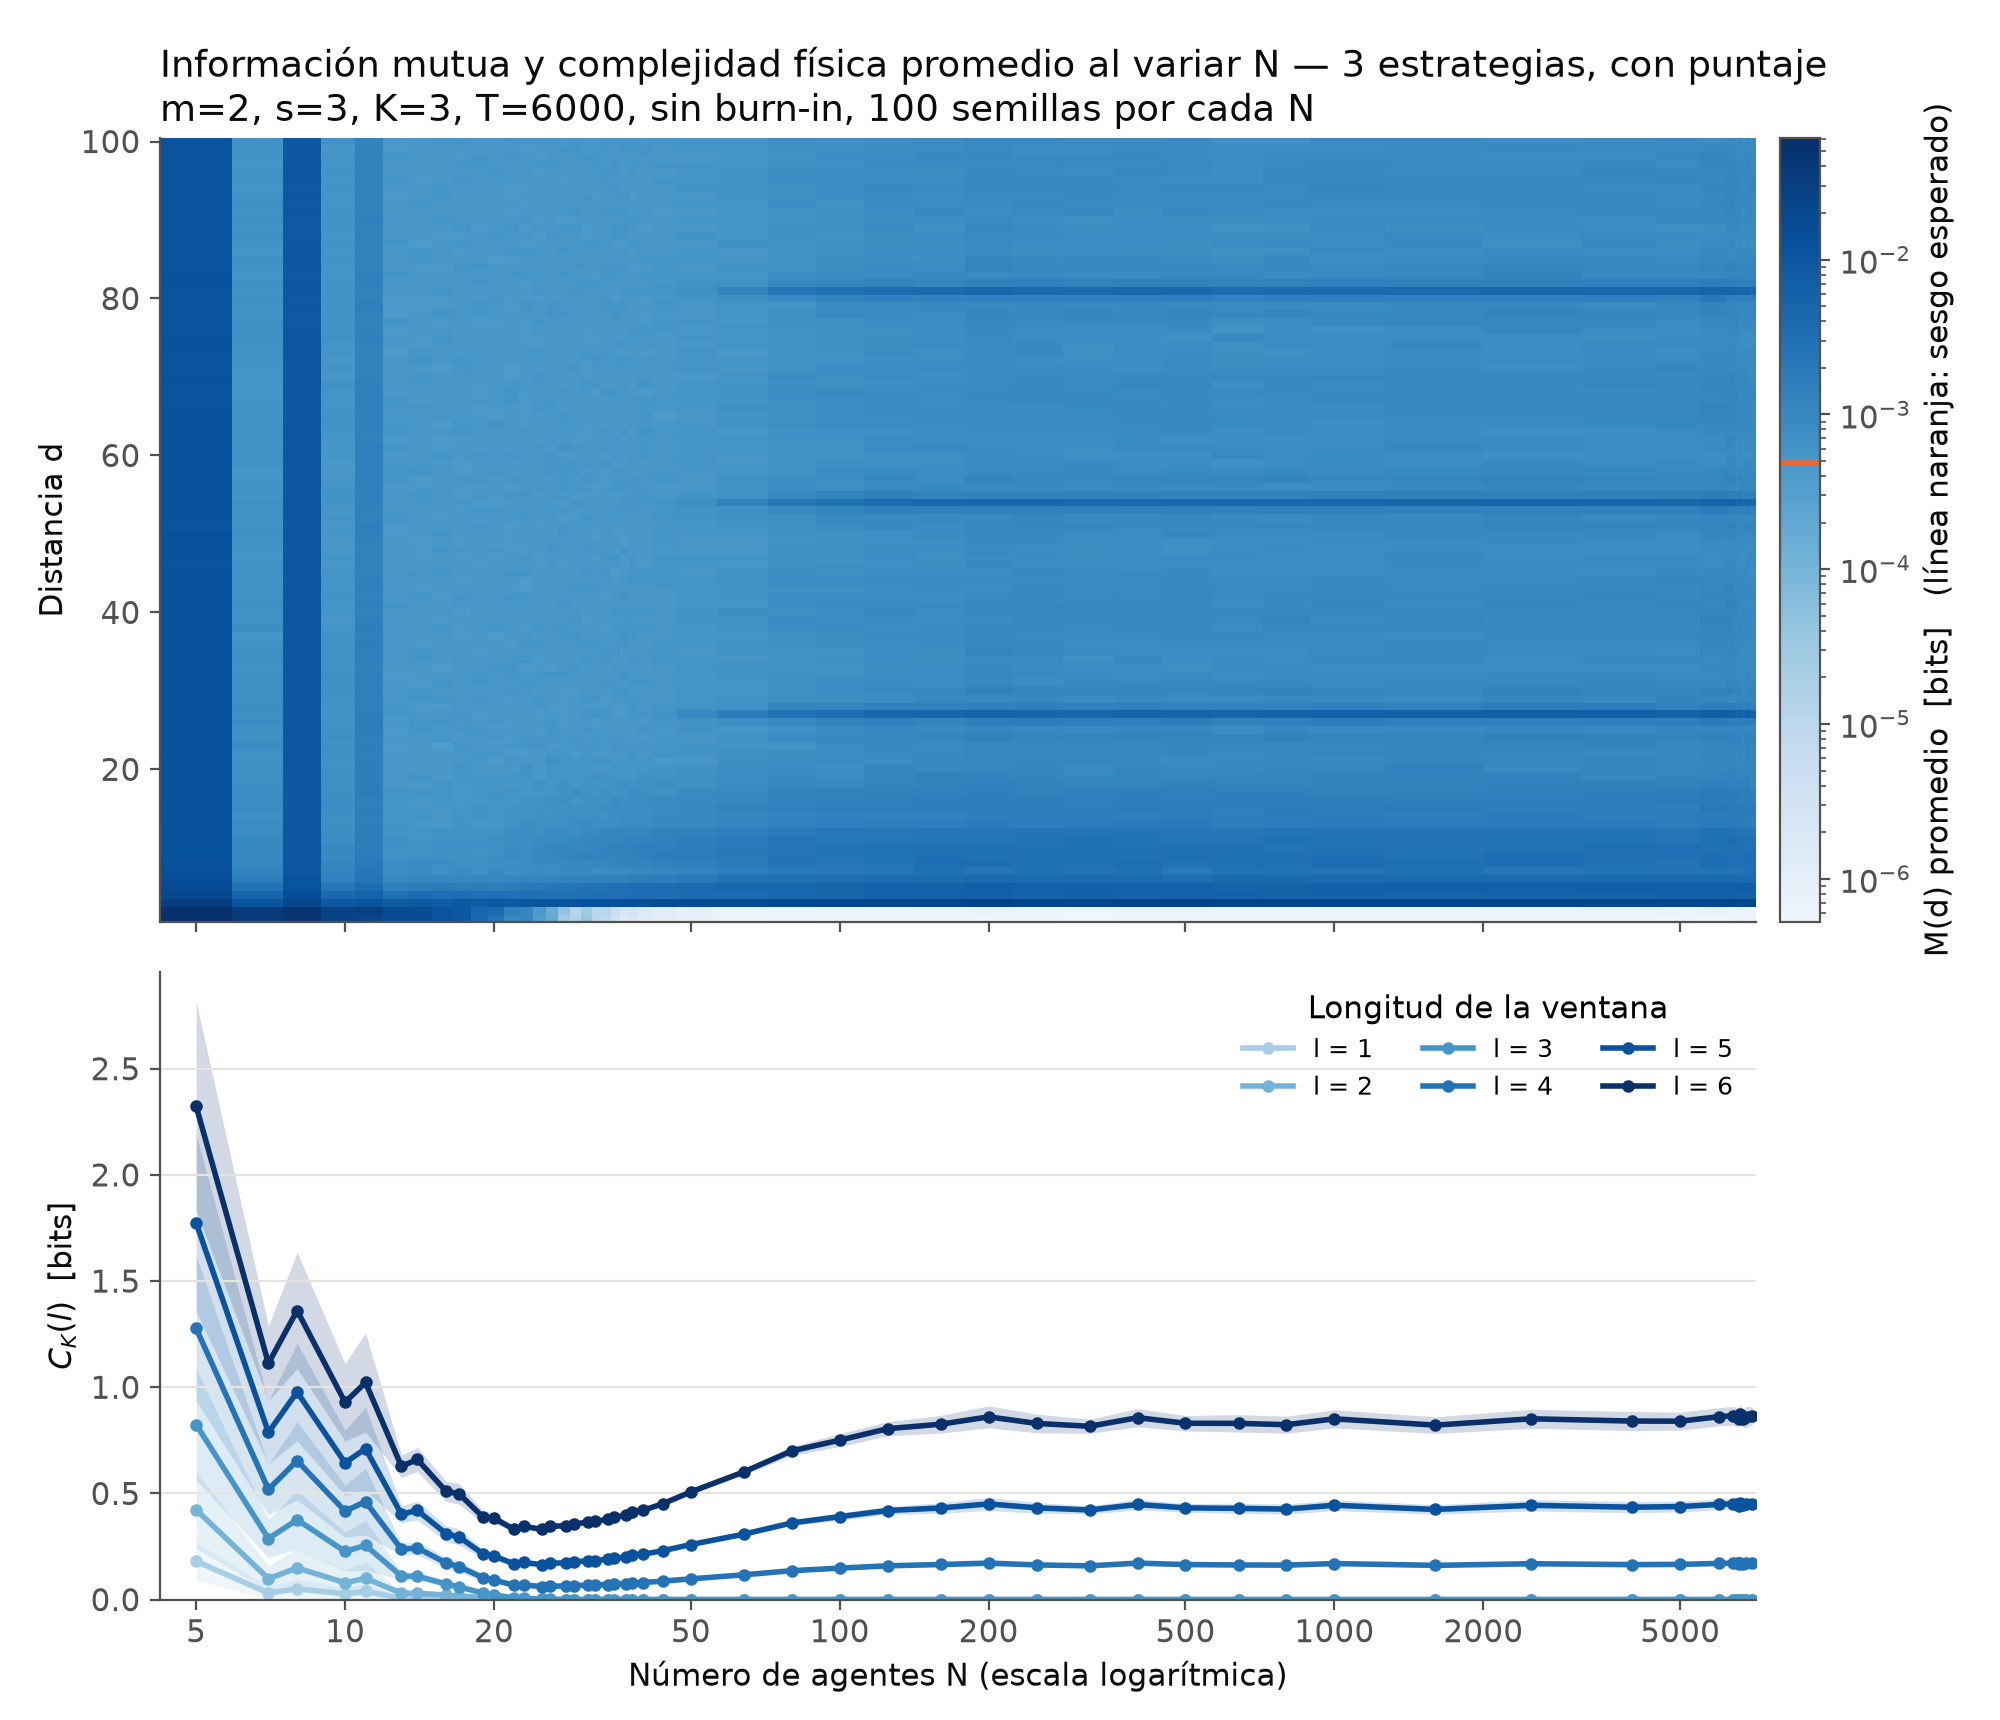
\includegraphics[width=0.86\textwidth]{figuras/Fase6_resumen_Md_CK_con_puntaje_m2_s3_T6000_N5-a-7000_52valores.png}
\caption{Fase 6, resumen de los 52 valores de $N$. Arriba: $M(d)$ promedio en escala de color. Abajo: $C_K(l)$ promedio, con su intervalo de confianza.}\label{fig:f6}
\end{figure}

\subsection*{Observaciones}
\begin{itemize}
\item \textbf{$N$ chico.} Hasta $N=17$ ($\gamma\ge 0.53$), $M(d)$ tiene su máximo en $d=1$ o $d=2$, y $M(1)$ es del orden de $10^{-2}$. A partir de $N=19$ el máximo pasa a $d=3=m+1$.
\item \textbf{Caída de $M(1)$.} $M(1)$ baja de $6.1\times10^{-2}$ en $N=5$ a $1.0\times10^{-3}$ en $N=22$ y a $2.9\times10^{-5}$ en $N=28$, y desde $N\approx 64$ se mantiene cerca de $6\times10^{-7}$ bits. El cambio más fuerte está entre $N\approx 19$ y $N\approx 32$, es decir, $\gamma\approx 0.47$ a $0.28$.
\item \textbf{$N$ grande.} $M(3)$ crece hasta $2.3\times10^{-2}$ en $N=100$ y después oscila entre $2.2\times10^{-2}$ y $2.5\times10^{-2}$. Desde $N\approx 64$ se distinguen picos en $d=27$, 54 y 81, múltiplos de $3^{m+1}=27$.
\item \textbf{Complejidad.} $C_K(6)$ vale 2.32 en $N=5$, baja de forma no monótona hasta un mínimo de 0.33 en $N\approx 22$ a 25 ($\gamma\approx 0.41$ a $0.36$), y sube hasta estabilizarse entre 0.80 y 0.87 desde $N=125$. Para $N\ge 44$, $C_K(l)$ es prácticamente cero en $l\le 3=m+1$.
\item \textbf{Éxito de los agentes.} La tasa de éxito supera a la de agentes al azar hasta $N=31$ y queda por debajo desde $N=32$.
\end{itemize}

\begin{small}
\begin{longtable}{rrrrrrrrr}
\caption{Fase 6: resumen de los 52 valores de $N$ ($m=2$, $s=3$, $K=3$, $T=6000$, promedio de 100 cadenas). ``Éxito'' es la tasa de acierto de los agentes y ``Azar'' la de agentes que eligen al azar; $d_{\max}$ es la distancia donde $M(d)$ es máxima.}\label{tab:f6}\\
\toprule
$N$ & $\gamma$ & Éxito & Azar & $M(1)$ & $M(3)$ & $d_{\max}$ & $C_K(6)$ & $c_K(6)$ \\
\midrule
\endfirsthead
\toprule
$N$ & $\gamma$ & Éxito & Azar & $M(1)$ & $M(3)$ & $d_{\max}$ & $C_K(6)$ & $c_K(6)$ \\
\midrule
\endhead
\bottomrule
\endfoot
5 & 1.8000 & 0.1550 & 0.1231 & $6.14\times10^{-2}$ & $2.97\times10^{-2}$ & 1 & 2.323 & 0.2443 \\
7 & 1.2857 & 0.2009 & 0.1593 & $3.62\times10^{-2}$ & $1.09\times10^{-2}$ & 2 & 1.113 & 0.1170 \\
8 & 1.1250 & 0.2068 & 0.1664 & $4.74\times10^{-2}$ & $2.16\times10^{-2}$ & 2 & 1.361 & 0.1431 \\
10 & 0.9000 & 0.2319 & 0.1853 & $2.56\times10^{-2}$ & $9.30\times10^{-3}$ & 2 & 0.929 & 0.0977 \\
11 & 0.8182 & 0.2359 & 0.1902 & $2.34\times10^{-2}$ & $1.09\times10^{-2}$ & 2 & 1.022 & 0.1075 \\
13 & 0.6923 & 0.2500 & 0.2026 & $1.72\times10^{-2}$ & $7.65\times10^{-3}$ & 2 & 0.628 & 0.0660 \\
14 & 0.6429 & 0.2513 & 0.2061 & $1.80\times10^{-2}$ & $9.03\times10^{-3}$ & 1 & 0.660 & 0.0694 \\
16 & 0.5625 & 0.2606 & 0.2149 & $1.17\times10^{-2}$ & $8.14\times10^{-3}$ & 2 & 0.510 & 0.0536 \\
17 & 0.5294 & 0.2601 & 0.2176 & $9.52\times10^{-3}$ & $9.33\times10^{-3}$ & 1 & 0.498 & 0.0524 \\
19 & 0.4737 & 0.2630 & 0.2243 & $4.29\times10^{-3}$ & $8.41\times10^{-3}$ & 3 & 0.389 & 0.0409 \\
20 & 0.4500 & 0.2622 & 0.2265 & $2.72\times10^{-3}$ & $9.10\times10^{-3}$ & 3 & 0.383 & 0.0403 \\
22 & 0.4091 & 0.2606 & 0.2317 & $1.01\times10^{-3}$ & $8.44\times10^{-3}$ & 3 & 0.330 & 0.0347 \\
23 & 0.3913 & 0.2586 & 0.2335 & $1.06\times10^{-3}$ & $9.72\times10^{-3}$ & 3 & 0.345 & 0.0363 \\
25 & 0.3600 & 0.2560 & 0.2378 & $3.42\times10^{-4}$ & $1.05\times10^{-2}$ & 3 & 0.330 & 0.0348 \\
26 & 0.3462 & 0.2537 & 0.2393 & $1.72\times10^{-4}$ & $1.10\times10^{-2}$ & 3 & 0.346 & 0.0363 \\
28 & 0.3214 & 0.2511 & 0.2430 & $2.88\times10^{-5}$ & $1.14\times10^{-2}$ & 3 & 0.348 & 0.0365 \\
29 & 0.3103 & 0.2499 & 0.2442 & $1.41\times10^{-5}$ & $1.23\times10^{-2}$ & 3 & 0.355 & 0.0374 \\
31 & 0.2903 & 0.2489 & 0.2473 & $3.92\times10^{-5}$ & $1.25\times10^{-2}$ & 3 & 0.365 & 0.0384 \\
32 & 0.2812 & 0.2479 & 0.2485 & $1.08\times10^{-5}$ & $1.31\times10^{-2}$ & 3 & 0.368 & 0.0387 \\
34 & 0.2647 & 0.2467 & 0.2511 & $8.29\times10^{-6}$ & $1.32\times10^{-2}$ & 3 & 0.378 & 0.0398 \\
35 & 0.2571 & 0.2457 & 0.2521 & $4.10\times10^{-6}$ & $1.35\times10^{-2}$ & 3 & 0.387 & 0.0407 \\
37 & 0.2432 & 0.2449 & 0.2544 & $1.68\times10^{-6}$ & $1.43\times10^{-2}$ & 3 & 0.398 & 0.0419 \\
38 & 0.2368 & 0.2442 & 0.2553 & $2.40\times10^{-6}$ & $1.48\times10^{-2}$ & 3 & 0.414 & 0.0435 \\
40 & 0.2250 & 0.2431 & 0.2574 & $1.36\times10^{-6}$ & $1.48\times10^{-2}$ & 3 & 0.420 & 0.0442 \\
44 & 0.2045 & 0.2418 & 0.2608 & $1.19\times10^{-6}$ & $1.60\times10^{-2}$ & 3 & 0.452 & 0.0476 \\
50 & 0.1800 & 0.2404 & 0.2652 & $8.24\times10^{-7}$ & $1.67\times10^{-2}$ & 3 & 0.507 & 0.0533 \\
64 & 0.1406 & 0.2395 & 0.2730 & $6.31\times10^{-7}$ & $1.83\times10^{-2}$ & 3 & 0.602 & 0.0633 \\
80 & 0.1125 & 0.2396 & 0.2792 & $6.67\times10^{-7}$ & $2.12\times10^{-2}$ & 3 & 0.700 & 0.0736 \\
100 & 0.0900 & 0.2406 & 0.2849 & $5.87\times10^{-7}$ & $2.35\times10^{-2}$ & 3 & 0.751 & 0.0790 \\
125 & 0.0720 & 0.2410 & 0.2901 & $6.20\times10^{-7}$ & $2.31\times10^{-2}$ & 3 & 0.805 & 0.0846 \\
160 & 0.0563 & 0.2421 & 0.2950 & $6.00\times10^{-7}$ & $2.28\times10^{-2}$ & 3 & 0.826 & 0.0869 \\
200 & 0.0450 & 0.2434 & 0.2990 & $6.23\times10^{-7}$ & $2.50\times10^{-2}$ & 3 & 0.860 & 0.0905 \\
250 & 0.0360 & 0.2447 & 0.3026 & $6.26\times10^{-7}$ & $2.22\times10^{-2}$ & 3 & 0.830 & 0.0872 \\
320 & 0.0281 & 0.2454 & 0.3062 & $5.24\times10^{-7}$ & $2.24\times10^{-2}$ & 3 & 0.816 & 0.0858 \\
400 & 0.0225 & 0.2463 & 0.3090 & $6.40\times10^{-7}$ & $2.42\times10^{-2}$ & 3 & 0.857 & 0.0901 \\
500 & 0.0180 & 0.2472 & 0.3116 & $6.35\times10^{-7}$ & $2.47\times10^{-2}$ & 3 & 0.830 & 0.0873 \\
640 & 0.0141 & 0.2478 & 0.3141 & $5.75\times10^{-7}$ & $2.38\times10^{-2}$ & 3 & 0.830 & 0.0873 \\
800 & 0.0112 & 0.2484 & 0.3161 & $6.34\times10^{-7}$ & $2.46\times10^{-2}$ & 3 & 0.824 & 0.0866 \\
1000 & 0.0090 & 0.2488 & 0.3179 & $5.99\times10^{-7}$ & $2.30\times10^{-2}$ & 3 & 0.851 & 0.0895 \\
1600 & 0.0056 & 0.2497 & 0.3211 & $5.79\times10^{-7}$ & $2.26\times10^{-2}$ & 3 & 0.822 & 0.0864 \\
2500 & 0.0036 & 0.2502 & 0.3236 & $6.41\times10^{-7}$ & $2.36\times10^{-2}$ & 3 & 0.851 & 0.0895 \\
4000 & 0.0022 & 0.2509 & 0.3256 & $6.25\times10^{-7}$ & $2.21\times10^{-2}$ & 3 & 0.841 & 0.0884 \\
5000 & 0.0018 & 0.2509 & 0.3264 & $5.78\times10^{-7}$ & $2.31\times10^{-2}$ & 3 & 0.840 & 0.0884 \\
6001 & 0.0015 & 0.2509 & 0.3270 & $5.40\times10^{-7}$ & $2.15\times10^{-2}$ & 3 & 0.862 & 0.0906 \\
6400 & 0.0014 & 0.2510 & 0.3272 & $5.73\times10^{-7}$ & $2.44\times10^{-2}$ & 3 & 0.866 & 0.0910 \\
6500 & 0.0014 & 0.2511 & 0.3273 & $6.09\times10^{-7}$ & $2.26\times10^{-2}$ & 3 & 0.859 & 0.0903 \\
6560 & 0.0014 & 0.2507 & 0.3273 & $6.94\times10^{-7}$ & $2.16\times10^{-2}$ & 3 & 0.866 & 0.0910 \\
6562 & 0.0014 & 0.2510 & 0.3273 & $6.64\times10^{-7}$ & $2.18\times10^{-2}$ & 3 & 0.850 & 0.0894 \\
6601 & 0.0014 & 0.2511 & 0.3273 & $5.80\times10^{-7}$ & $2.26\times10^{-2}$ & 3 & 0.873 & 0.0918 \\
6700 & 0.0013 & 0.2512 & 0.3274 & $6.10\times10^{-7}$ & $2.34\times10^{-2}$ & 3 & 0.852 & 0.0896 \\
6800 & 0.0013 & 0.2511 & 0.3274 & $6.09\times10^{-7}$ & $2.36\times10^{-2}$ & 3 & 0.861 & 0.0905 \\
7000 & 0.0013 & 0.2510 & 0.3275 & $6.17\times10^{-7}$ & $2.24\times10^{-2}$ & 3 & 0.866 & 0.0911 \\
\end{longtable}
\end{small}


\section{Fase 7: variación de la memoria en el juego de 3 decisiones}
Con $N=101$ y $T=60000$ se varió $m$ de 1 a 6, para $s=2$ y $s=3$. La tabla~\ref{tab:f7} resume los resultados.

\begin{table}[H]
\centering
\footnotesize
\setlength{\tabcolsep}{3.5pt}
\caption{Fase 7: juego de 3 decisiones con $N=101$, $T=60000$. La tasa de éxito de agentes al azar es 0.2852. La pendiente y $R^2$ son los del ajuste log-log de $M(d)$ con $d=1,\dots,100$.}\label{tab:f7}
\begin{tabular}{rrrrrrrrrrr}
\toprule
$s$ & $m$ & $\gamma$ & Éxito & $M(1)$ & $M_{\max}$ & $d_{\max}$ & $C_K(6)$ & $c_K(6)$ & Pendiente & $R^2$ \\
\midrule
2 & 1 & 0.0297 & 0.2406 & $3.31\times10^{-9}$ & $1.99\times10^{-1}$ & 2 & 2.415 & 0.2539 & +0.5418 & 0.0825 \\
2 & 2 & 0.0891 & 0.2761 & $7.94\times10^{-9}$ & $1.83\times10^{-2}$ & 3 & 0.527 & 0.0555 & +0.0080 & 0.0000 \\
2 & 3 & 0.2673 & 0.3123 & $9.47\times10^{-3}$ & $1.19\times10^{-2}$ & 2 & 0.592 & 0.0623 & -1.0070 & 0.7501 \\
2 & 4 & 0.8020 & 0.3012 & $8.92\times10^{-3}$ & $1.02\times10^{-2}$ & 2 & 0.947 & 0.0996 & -1.0390 & 0.6918 \\
2 & 5 & 2.4059 & 0.2924 & $4.71\times10^{-3}$ & $4.71\times10^{-3}$ & 1 & 0.701 & 0.0737 & -0.9400 & 0.6561 \\
2 & 6 & 7.2178 & 0.2876 & $1.83\times10^{-3}$ & $1.83\times10^{-3}$ & 1 & 0.288 & 0.0303 & -0.7683 & 0.6359 \\
3 & 1 & 0.0297 & 0.1987 & $3.60\times10^{-9}$ & $1.71\times10^{-1}$ & 2 & 2.023 & 0.2128 & +0.5010 & 0.0735 \\
3 & 2 & 0.0891 & 0.2401 & $6.34\times10^{-9}$ & $2.34\times10^{-2}$ & 3 & 0.694 & 0.0730 & +0.3135 & 0.0266 \\
3 & 3 & 0.2673 & 0.2831 & $4.12\times10^{-8}$ & $3.25\times10^{-3}$ & 4 & 0.070 & 0.0073 & +0.3332 & 0.0473 \\
3 & 4 & 0.8020 & 0.3018 & $2.63\times10^{-3}$ & $2.63\times10^{-3}$ & 1 & 0.264 & 0.0278 & -0.6632 & 0.6015 \\
3 & 5 & 2.4059 & 0.2928 & $2.13\times10^{-3}$ & $2.13\times10^{-3}$ & 1 & 0.340 & 0.0357 & -0.6849 & 0.5748 \\
3 & 6 & 7.2178 & 0.2879 & $8.76\times10^{-4}$ & $9.08\times10^{-4}$ & 6 & 0.154 & 0.0162 & -0.5692 & 0.5629 \\
\bottomrule
\end{tabular}
\end{table}


\begin{figure}[H]
\centering
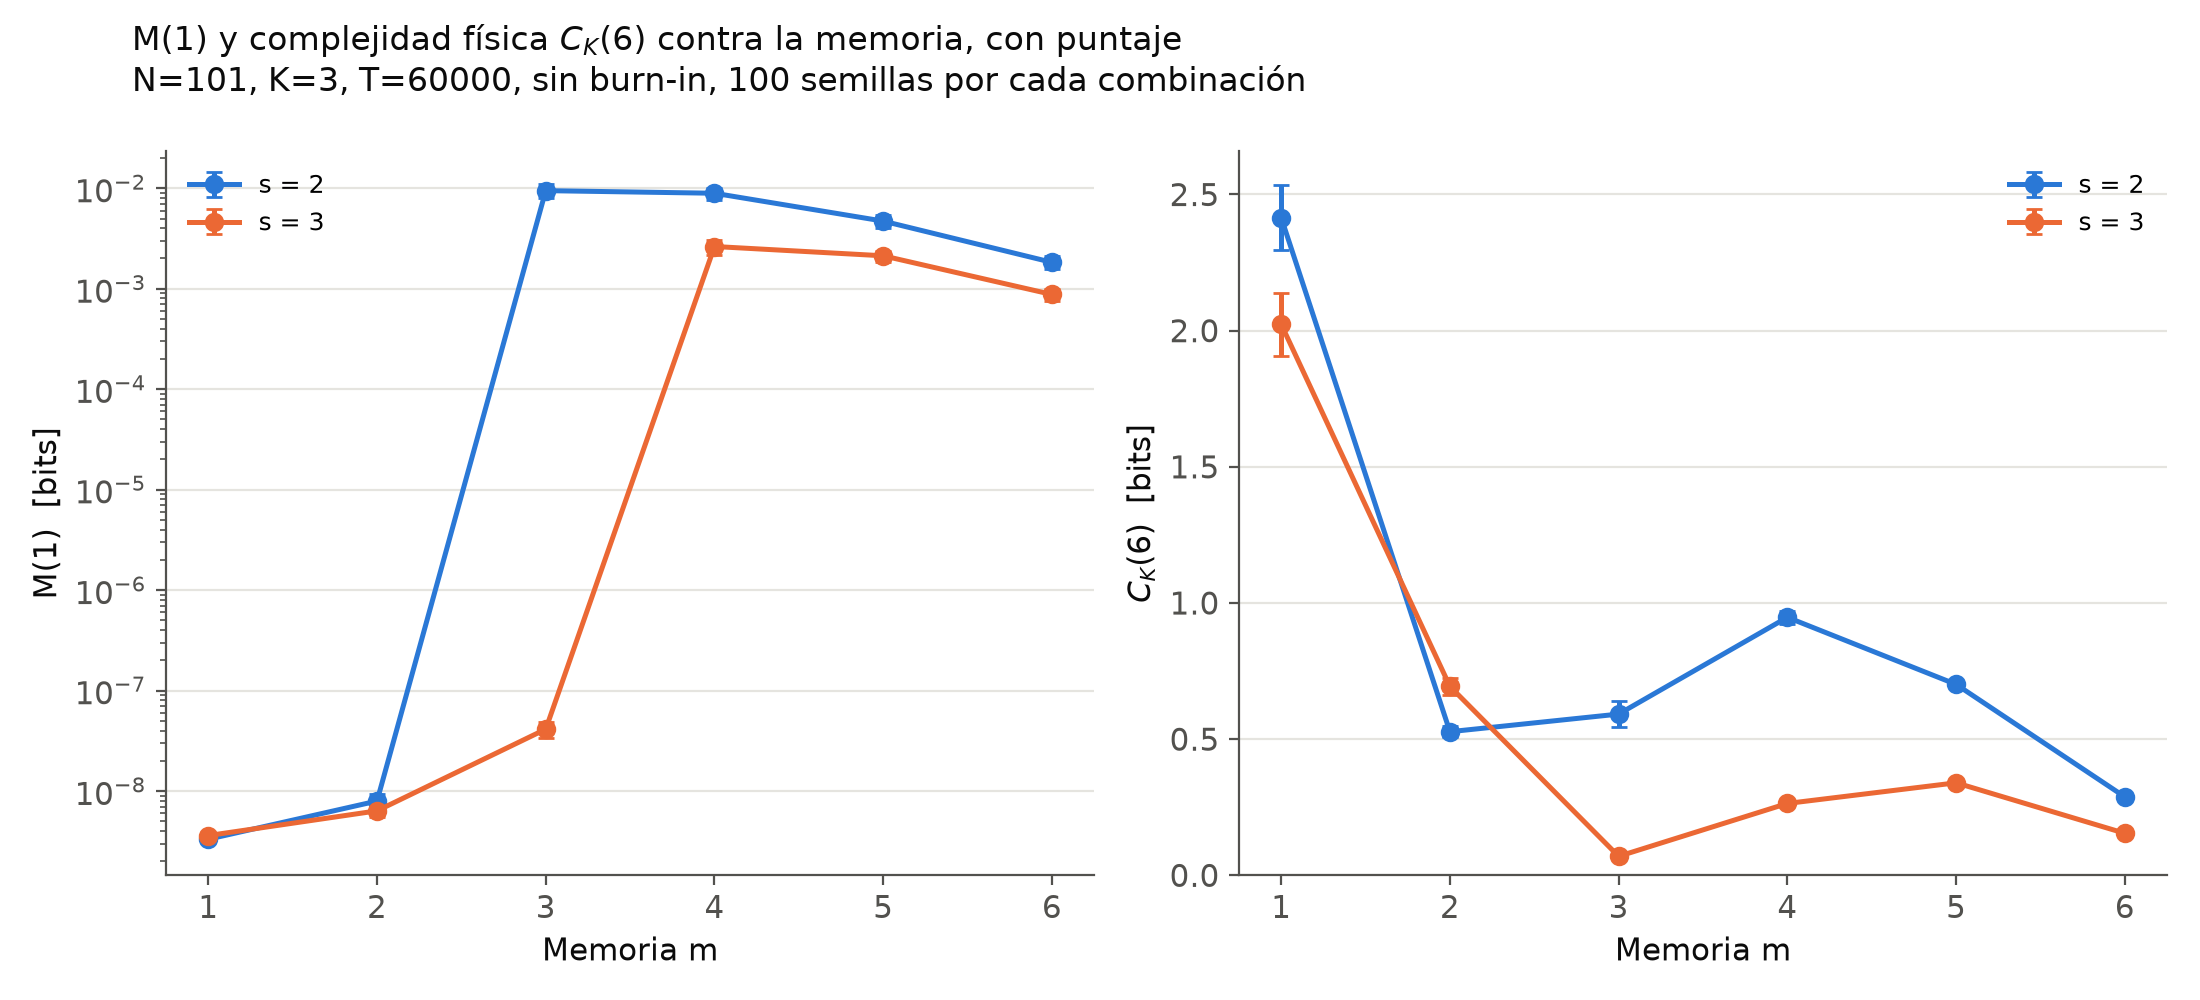
\includegraphics[width=0.8\textwidth]{figuras/Fase7_M1_CK6_contra_m_con_puntaje_N101_T60000.png}
\caption{Fase 7: $M(1)$ y $C_K(6)$ contra $m$, para $s=2$ y $s=3$.}\label{fig:f7m}
\end{figure}

\subsection*{Observaciones}
\begin{itemize}
\item \textbf{Con $s=2$ la forma cambia entre $m=2$ y $m=3$. Con $s=3$, entre $m=3$ y $m=4$.}
\item \textbf{Antes del cambio} ($s=2$: $m=1,2$; $s=3$: $m=1,2,3$), $M(d)$ es del orden de $10^{-8}$ bits para $d\le m$ y tiene su máximo en $d=m+1$, y $C_K(l)$ es cero hasta $l=m+1$.
\item \textbf{Después del cambio}, $M(d)$ es casi plana de $d=1$ a $d=m$ y luego cae, $C_K(l)$ es distinta de cero en todo $l$, y $M(1)$ salta a valores de $10^{-3}$ a $10^{-2}$ y disminuye con $m$.
\item \textbf{La tasa de éxito} supera a la de agentes al azar a partir de los mismos valores de $m$ en los que cambia la forma ($m=3$ con $s=2$ y $m=4$ con $s=3$).
\item \textbf{El ajuste log-log} da pendientes positivas o casi nulas y $R^2$ muy bajo antes del cambio, y después pendientes de $-0.57$ a $-1.04$, con $R^2$ de 0.56 a 0.75.
\item \textbf{Periodicidad.} Se observaron picos con periodo $K^{m+1}$ para $m=1$ (9) y $m=2$ (27). Con $s=3$, $m=3$ el periodo 81 no se observó, así que esa regularidad no vale en general.
\item \textbf{Consistencia con la fase 6.} Con $m=2$, $s=3$, $M(3)=2.34\times10^{-2}$, igual al de la fase 6 con $N=100$ ($2.3\times10^{-2}$).
\end{itemize}

\subsection*{Gráficas con $s=2$}
\begin{figure}[H]
\centering
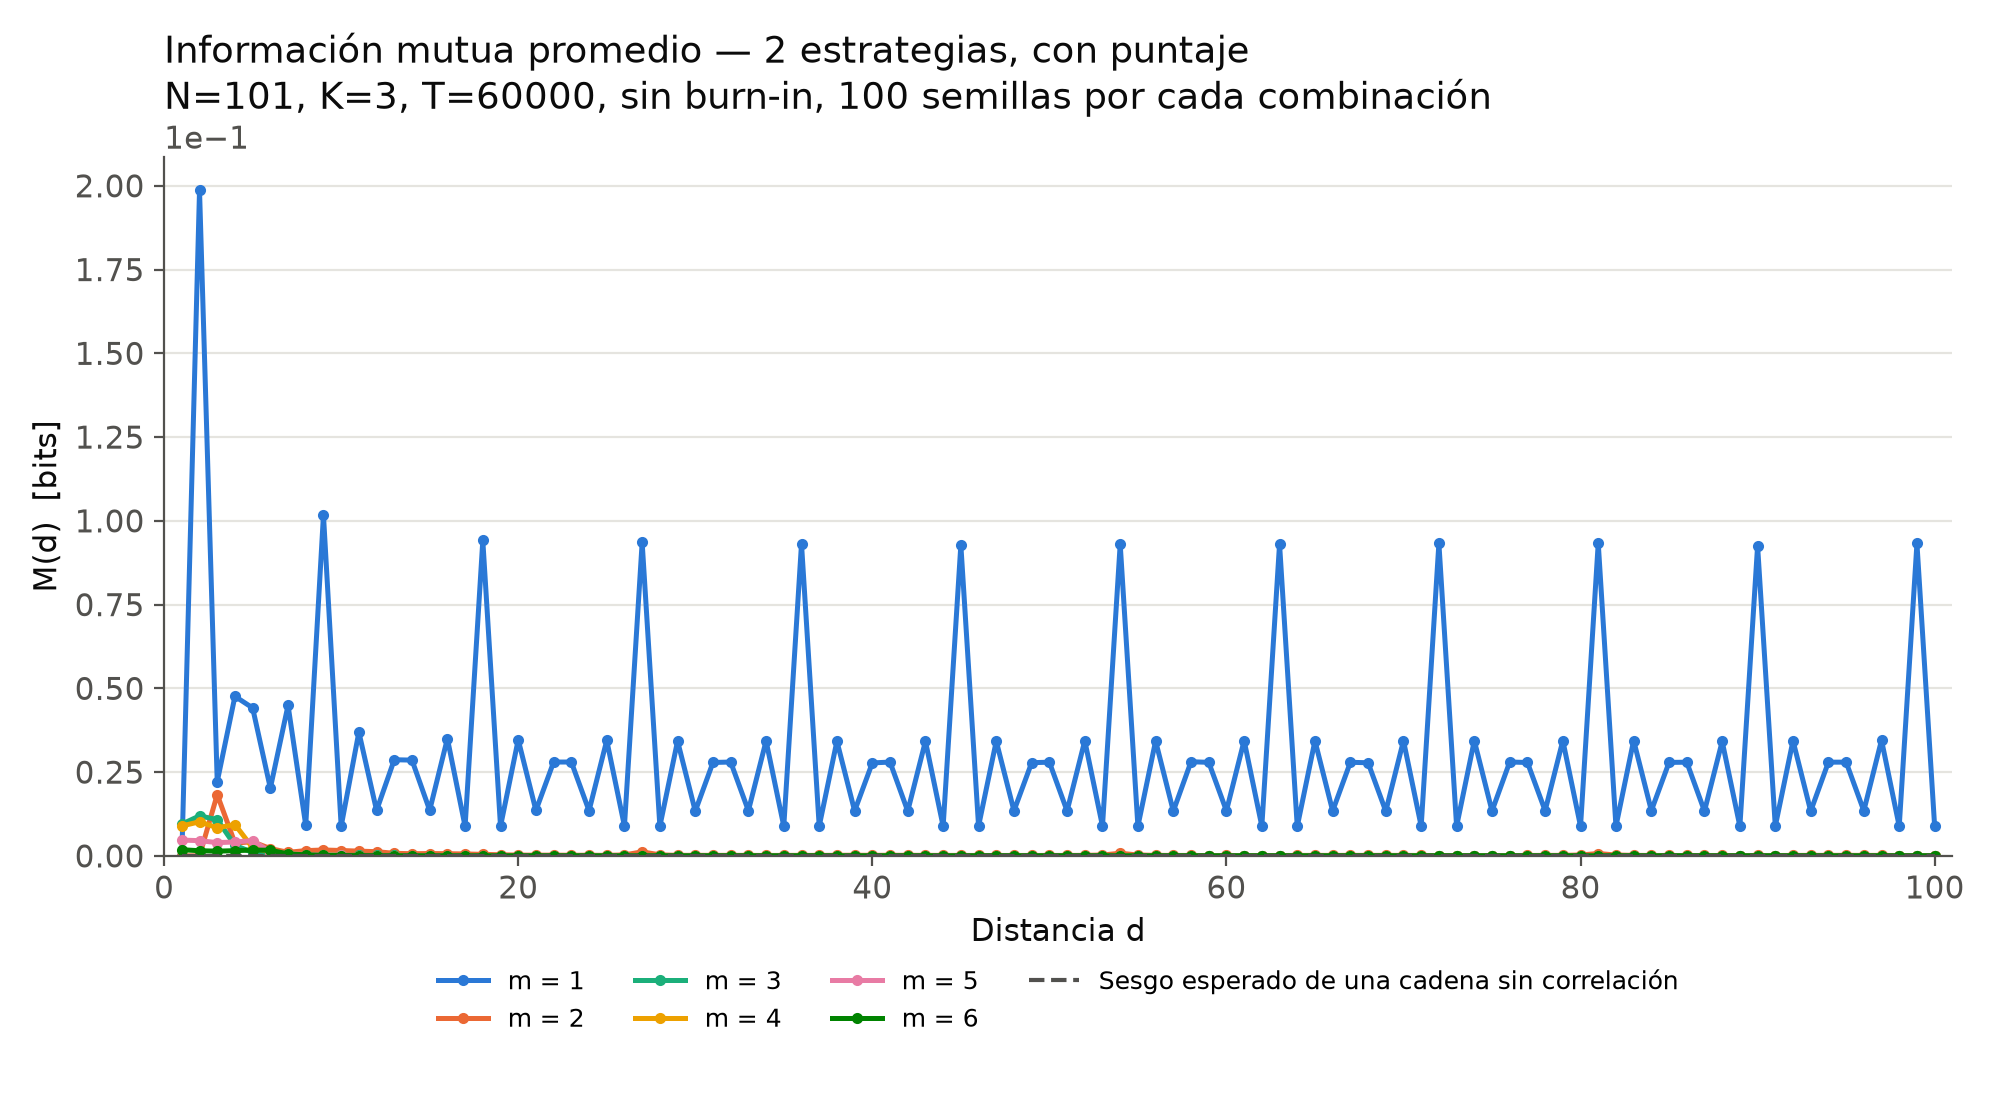
\includegraphics[width=0.92\textwidth]{figuras/Fase7_Md_con_puntaje_N101_s2_T60000_promedio.png}
\caption{Fase 7, $s=2$: $M(d)$ promedio, una curva por $m$. La línea punteada es el sesgo esperado de una cadena sin correlación.}
\end{figure}
\begin{figure}[H]
\centering
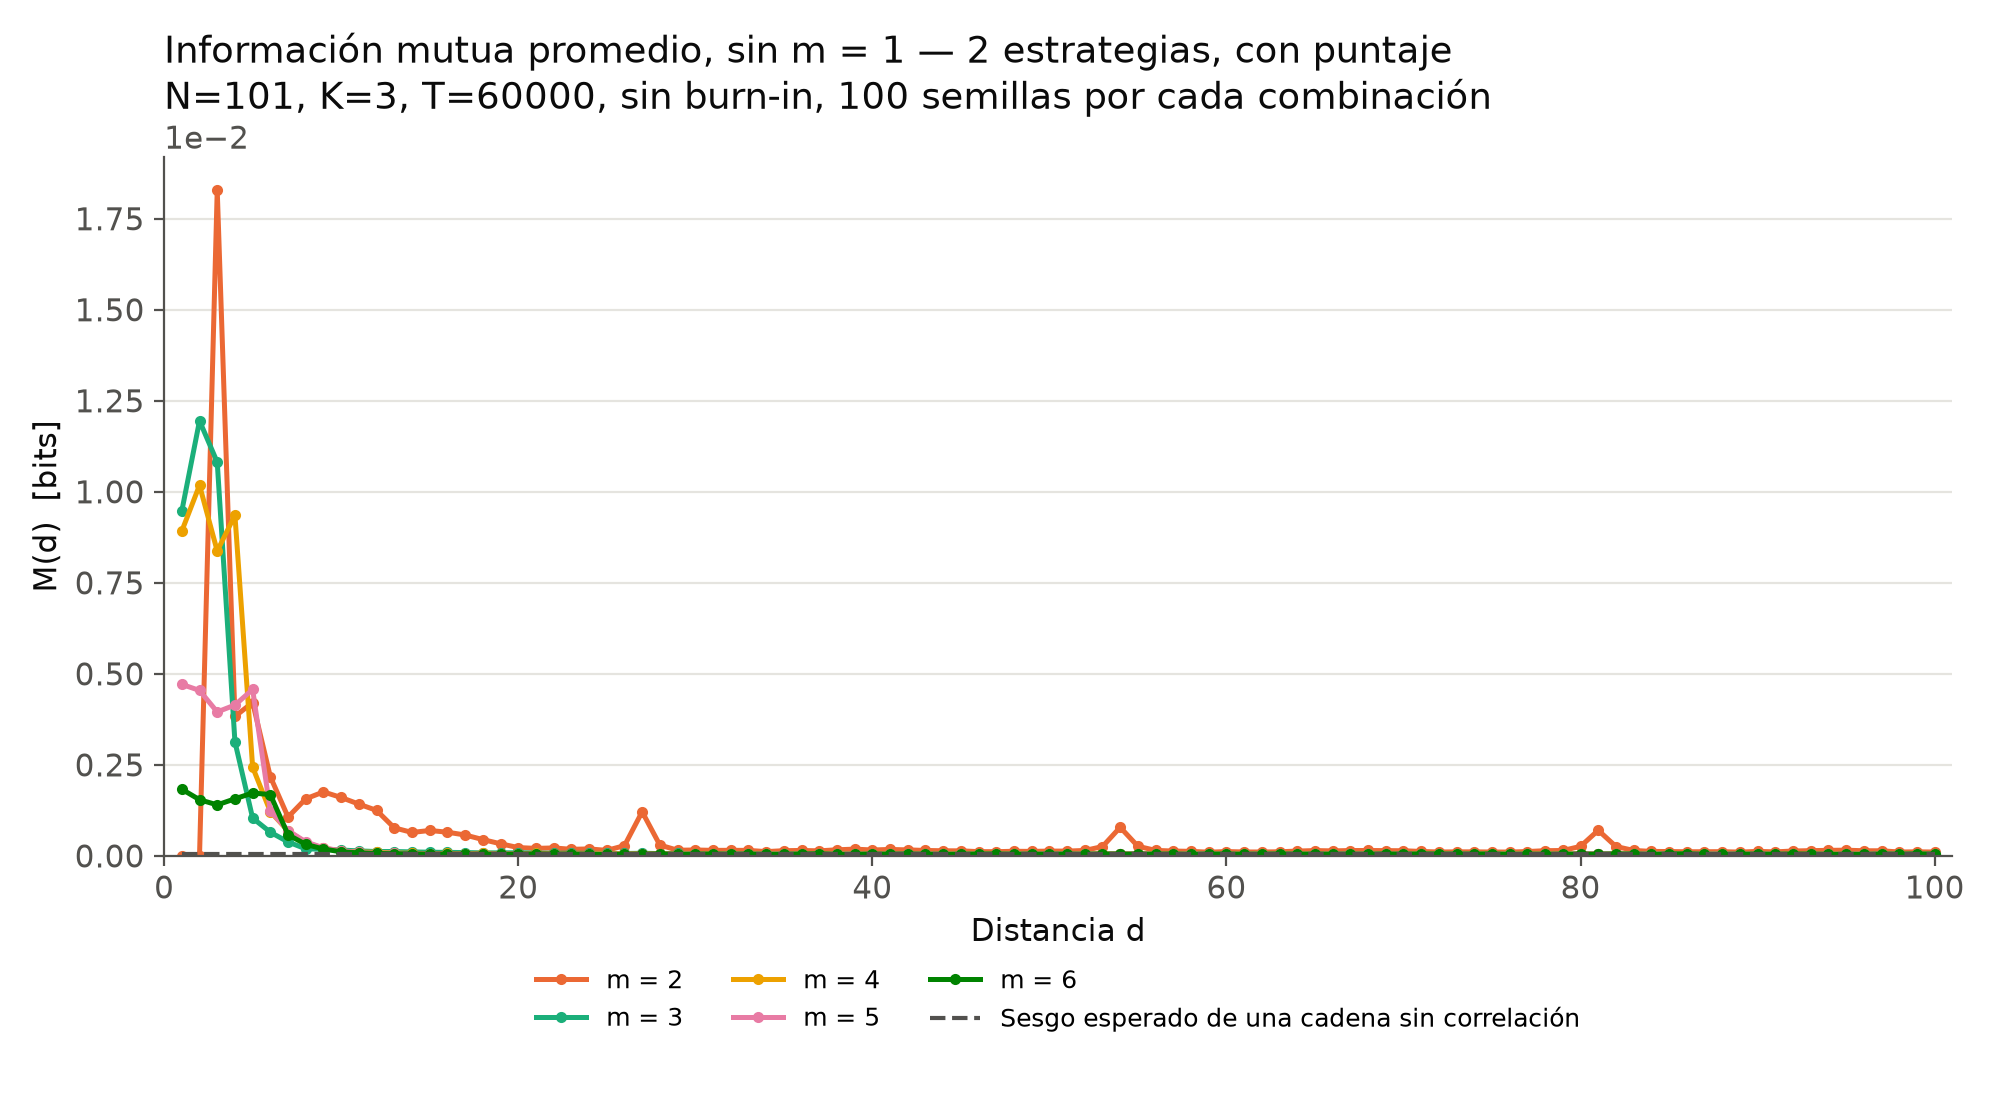
\includegraphics[width=0.92\textwidth]{figuras/Fase7_Md_sin_m1_con_puntaje_N101_s2_T60000_promedio.png}
\caption{Fase 7, $s=2$: la misma gráfica sin $m=1$.}
\end{figure}
\begin{figure}[H]
\centering
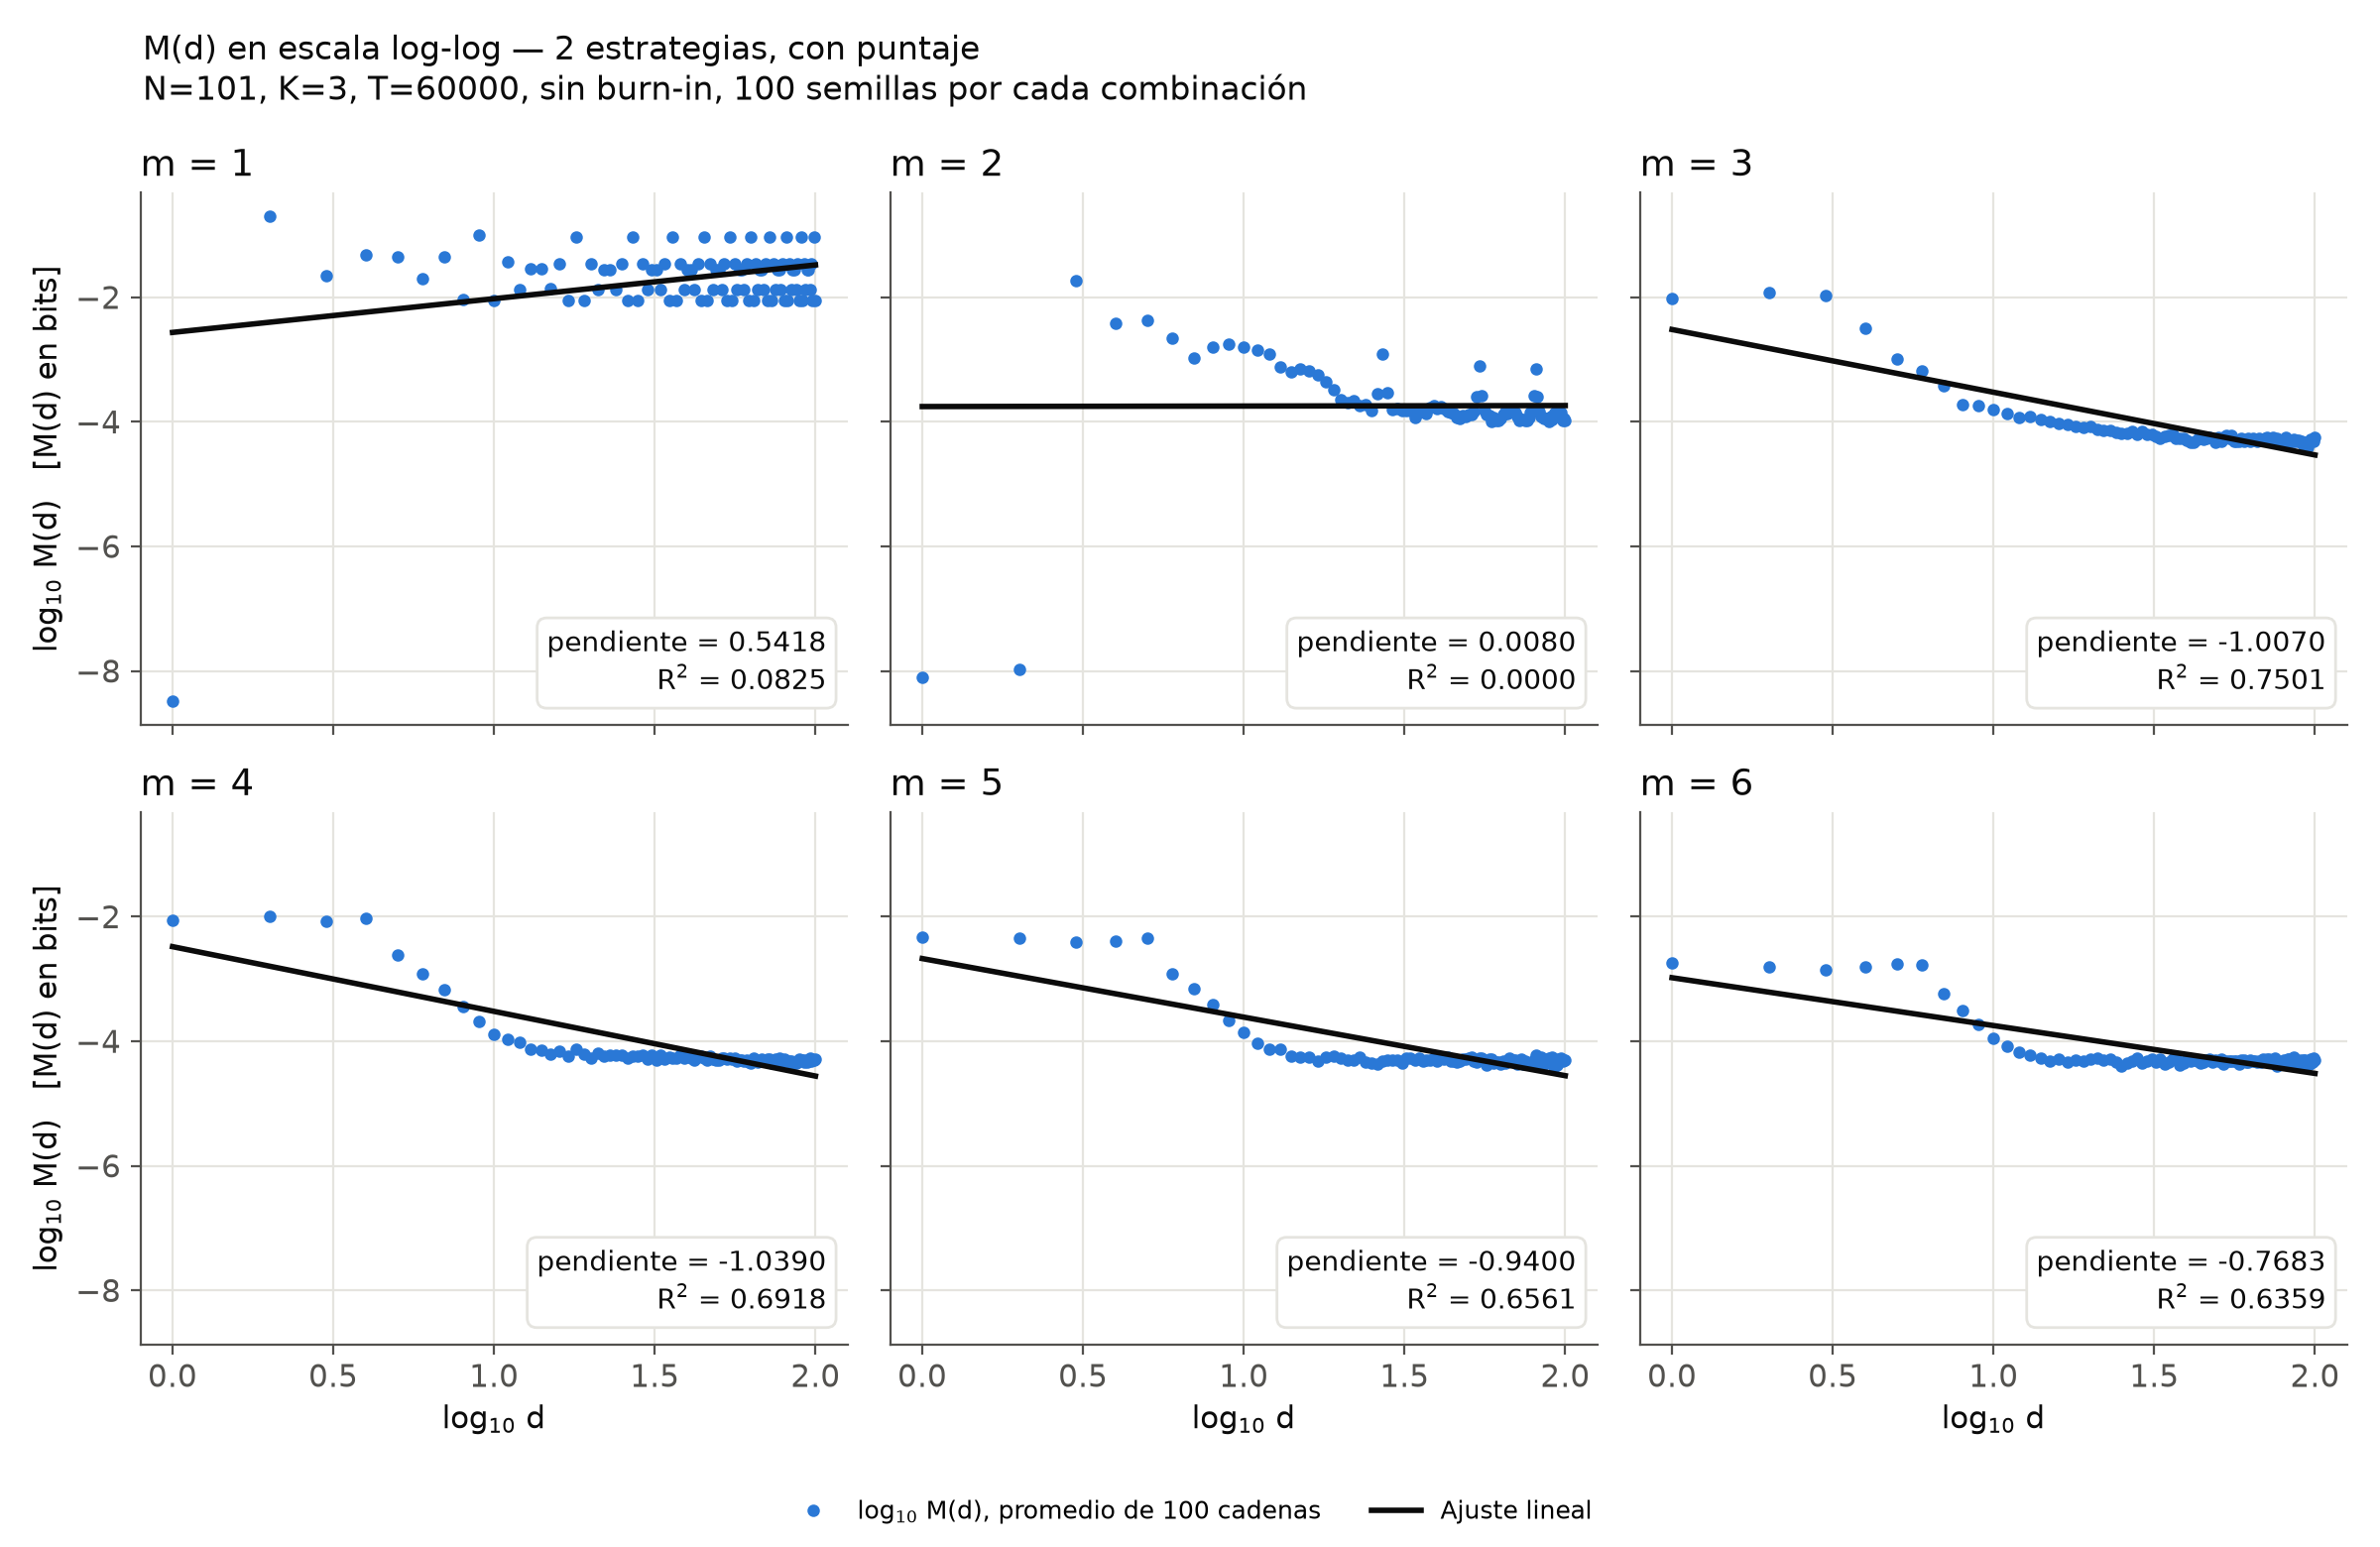
\includegraphics[width=0.92\textwidth]{figuras/Fase7_Md_loglog_con_puntaje_N101_s2_T60000_promedio.png}
\caption{Fase 7, $s=2$: $\log_{10} M(d)$ contra $\log_{10} d$, con su ajuste lineal.}
\end{figure}
\begin{figure}[H]
\centering
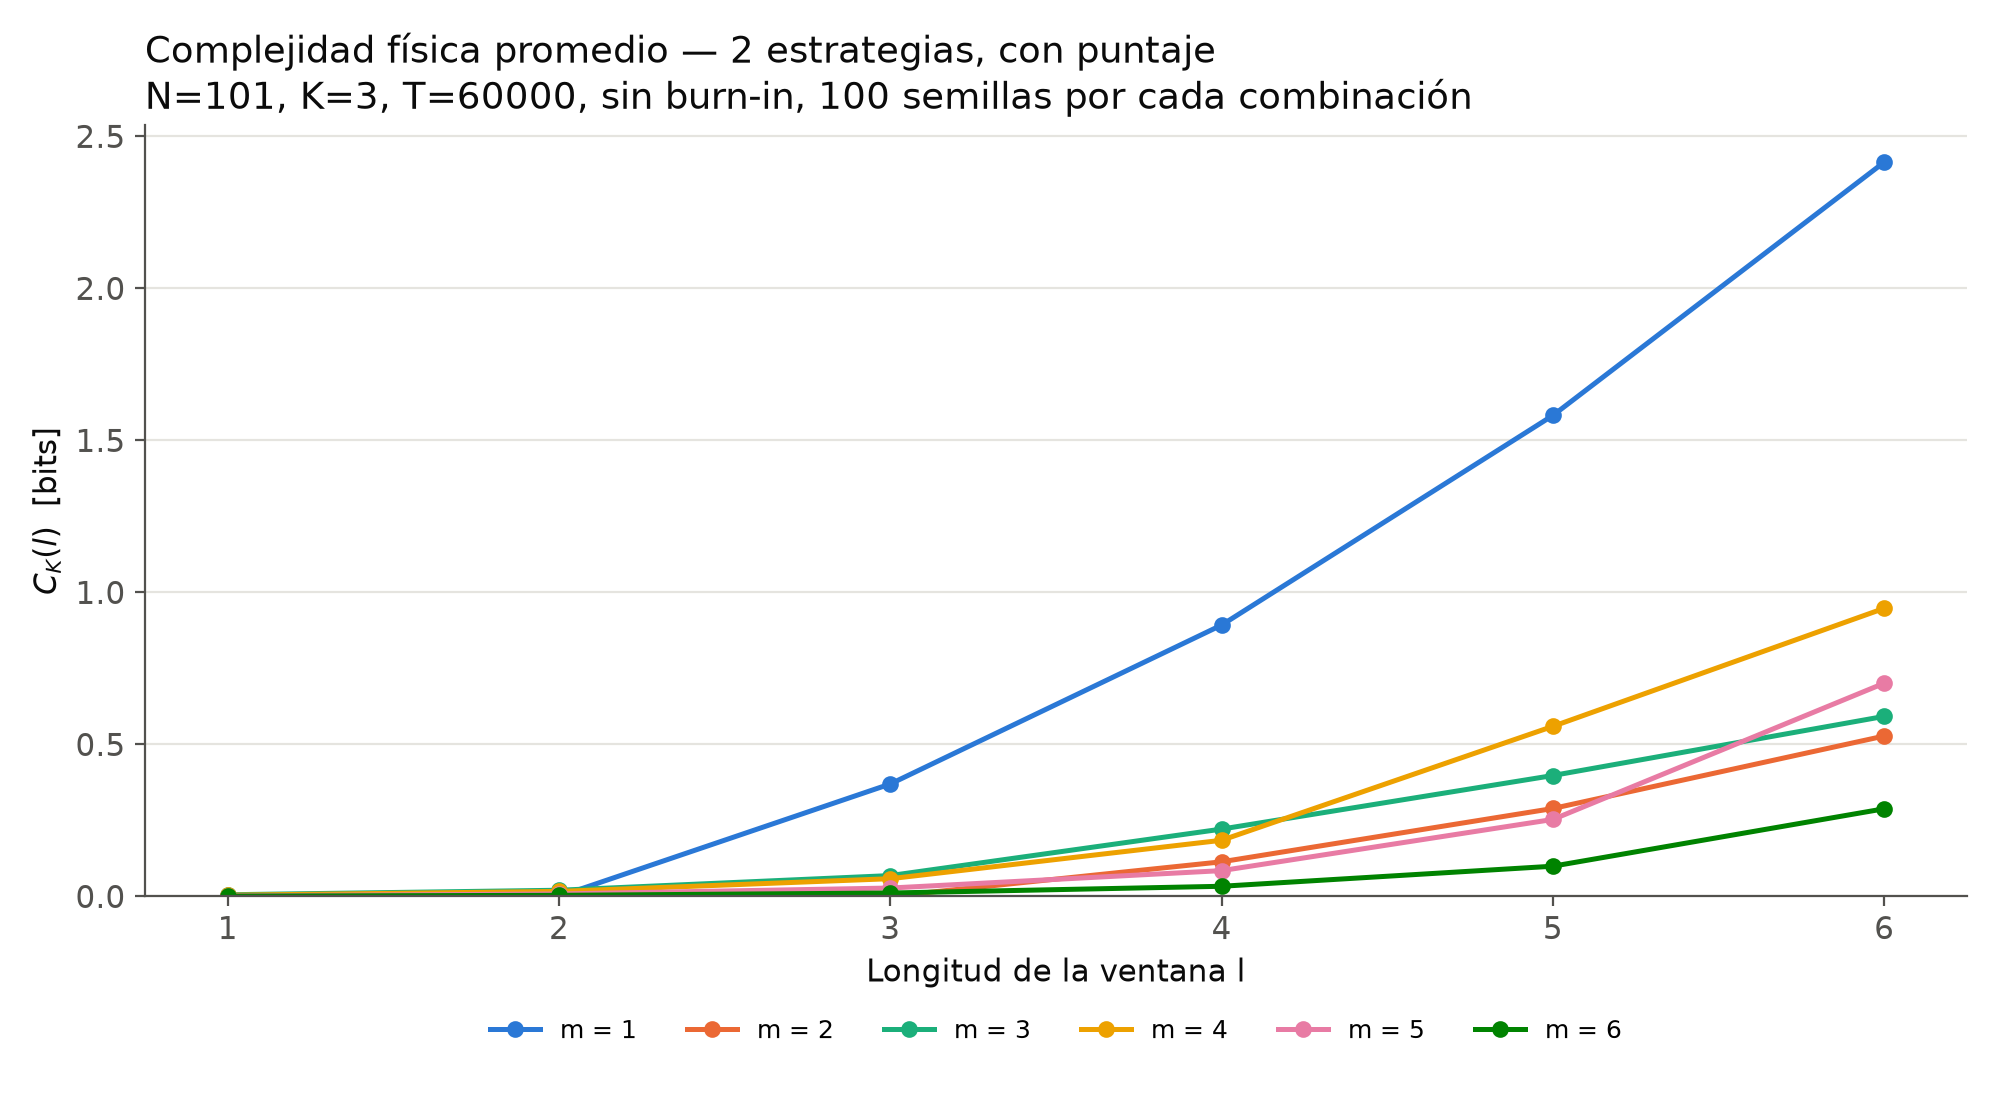
\includegraphics[width=0.92\textwidth]{figuras/Fase7_CK_con_puntaje_N101_s2_T60000_promedio.png}
\caption{Fase 7, $s=2$: $C_K(l)$ promedio contra $l$.}
\end{figure}

\subsection*{Gráficas con $s=3$}
\begin{figure}[H]
\centering
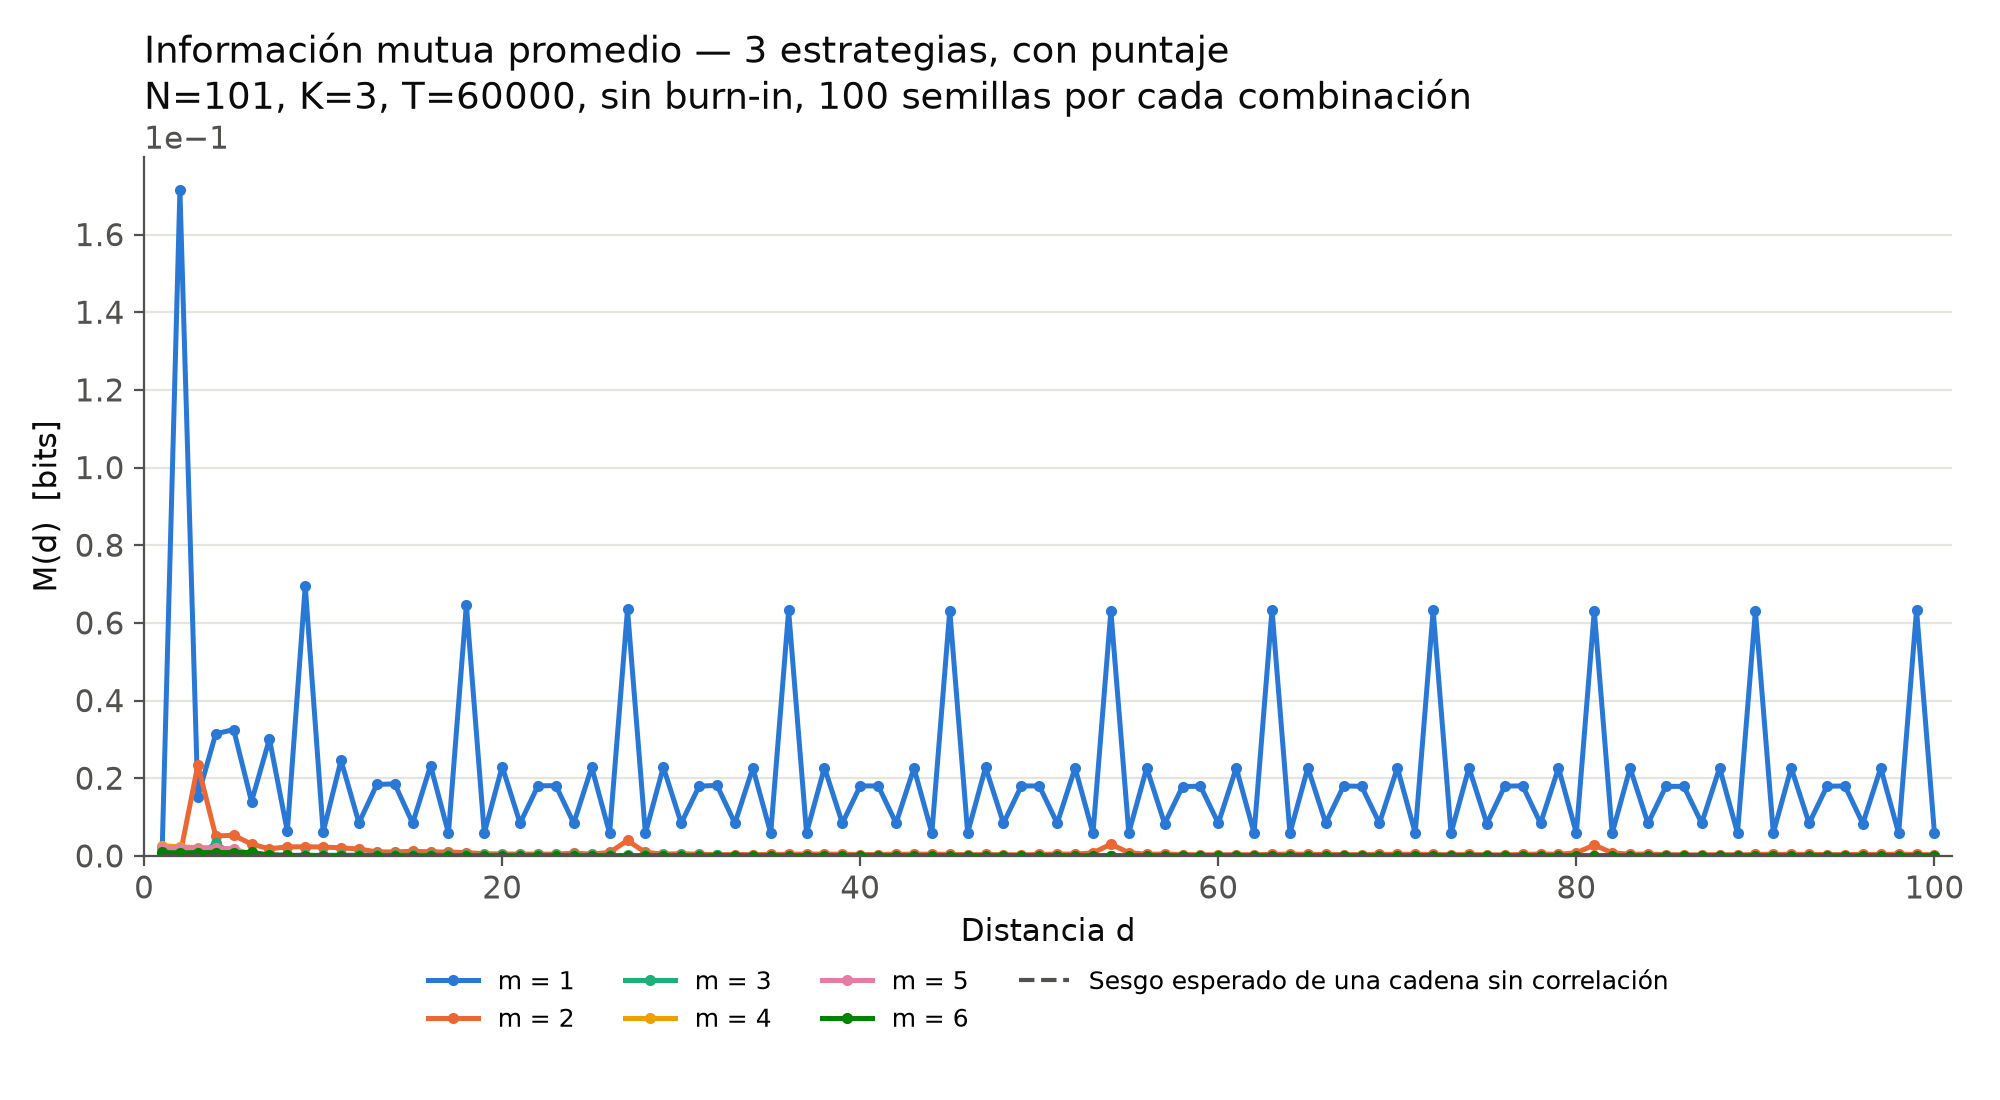
\includegraphics[width=0.92\textwidth]{figuras/Fase7_Md_con_puntaje_N101_s3_T60000_promedio.png}
\caption{Fase 7, $s=3$: $M(d)$ promedio, una curva por $m$. La línea punteada es el sesgo esperado de una cadena sin correlación.}
\end{figure}
\begin{figure}[H]
\centering
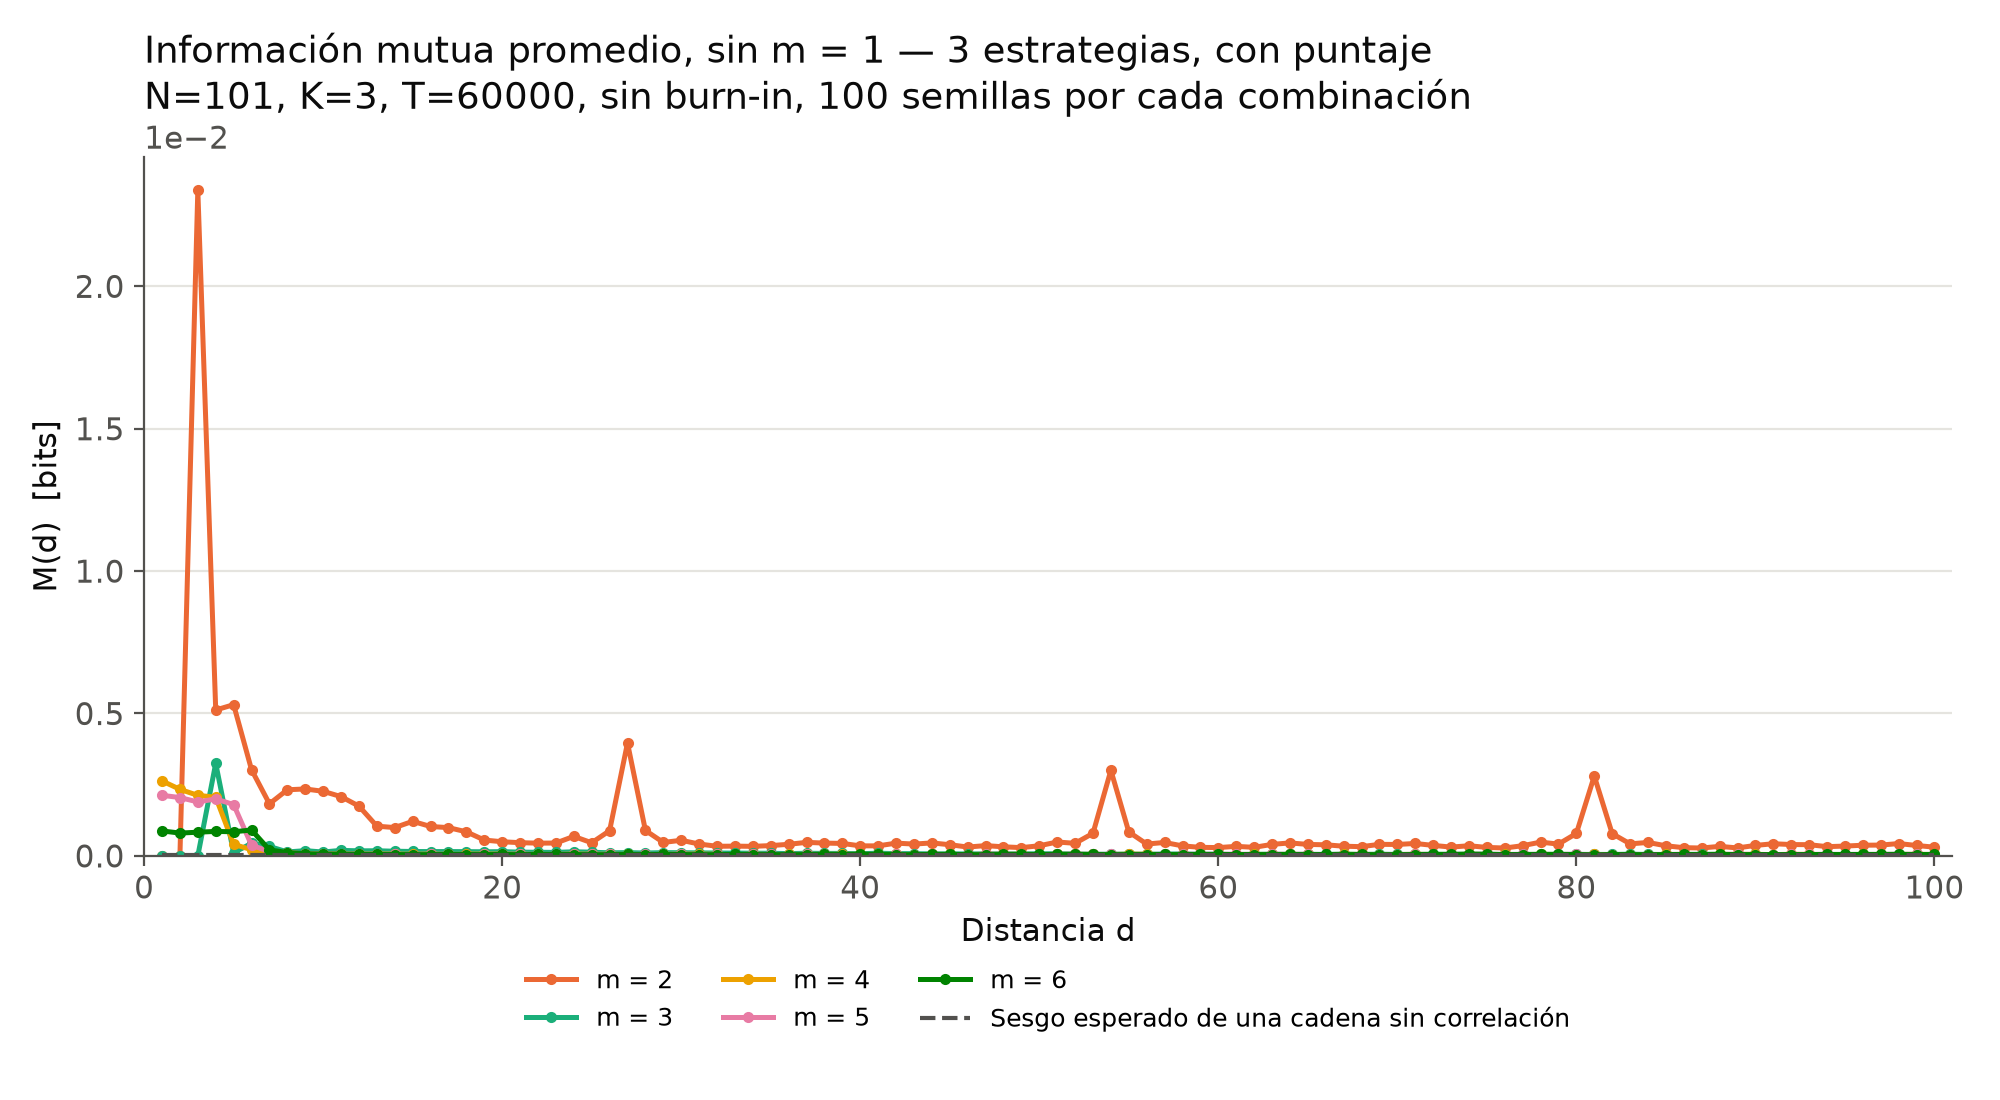
\includegraphics[width=0.92\textwidth]{figuras/Fase7_Md_sin_m1_con_puntaje_N101_s3_T60000_promedio.png}
\caption{Fase 7, $s=3$: la misma gráfica sin $m=1$.}
\end{figure}
\begin{figure}[H]
\centering
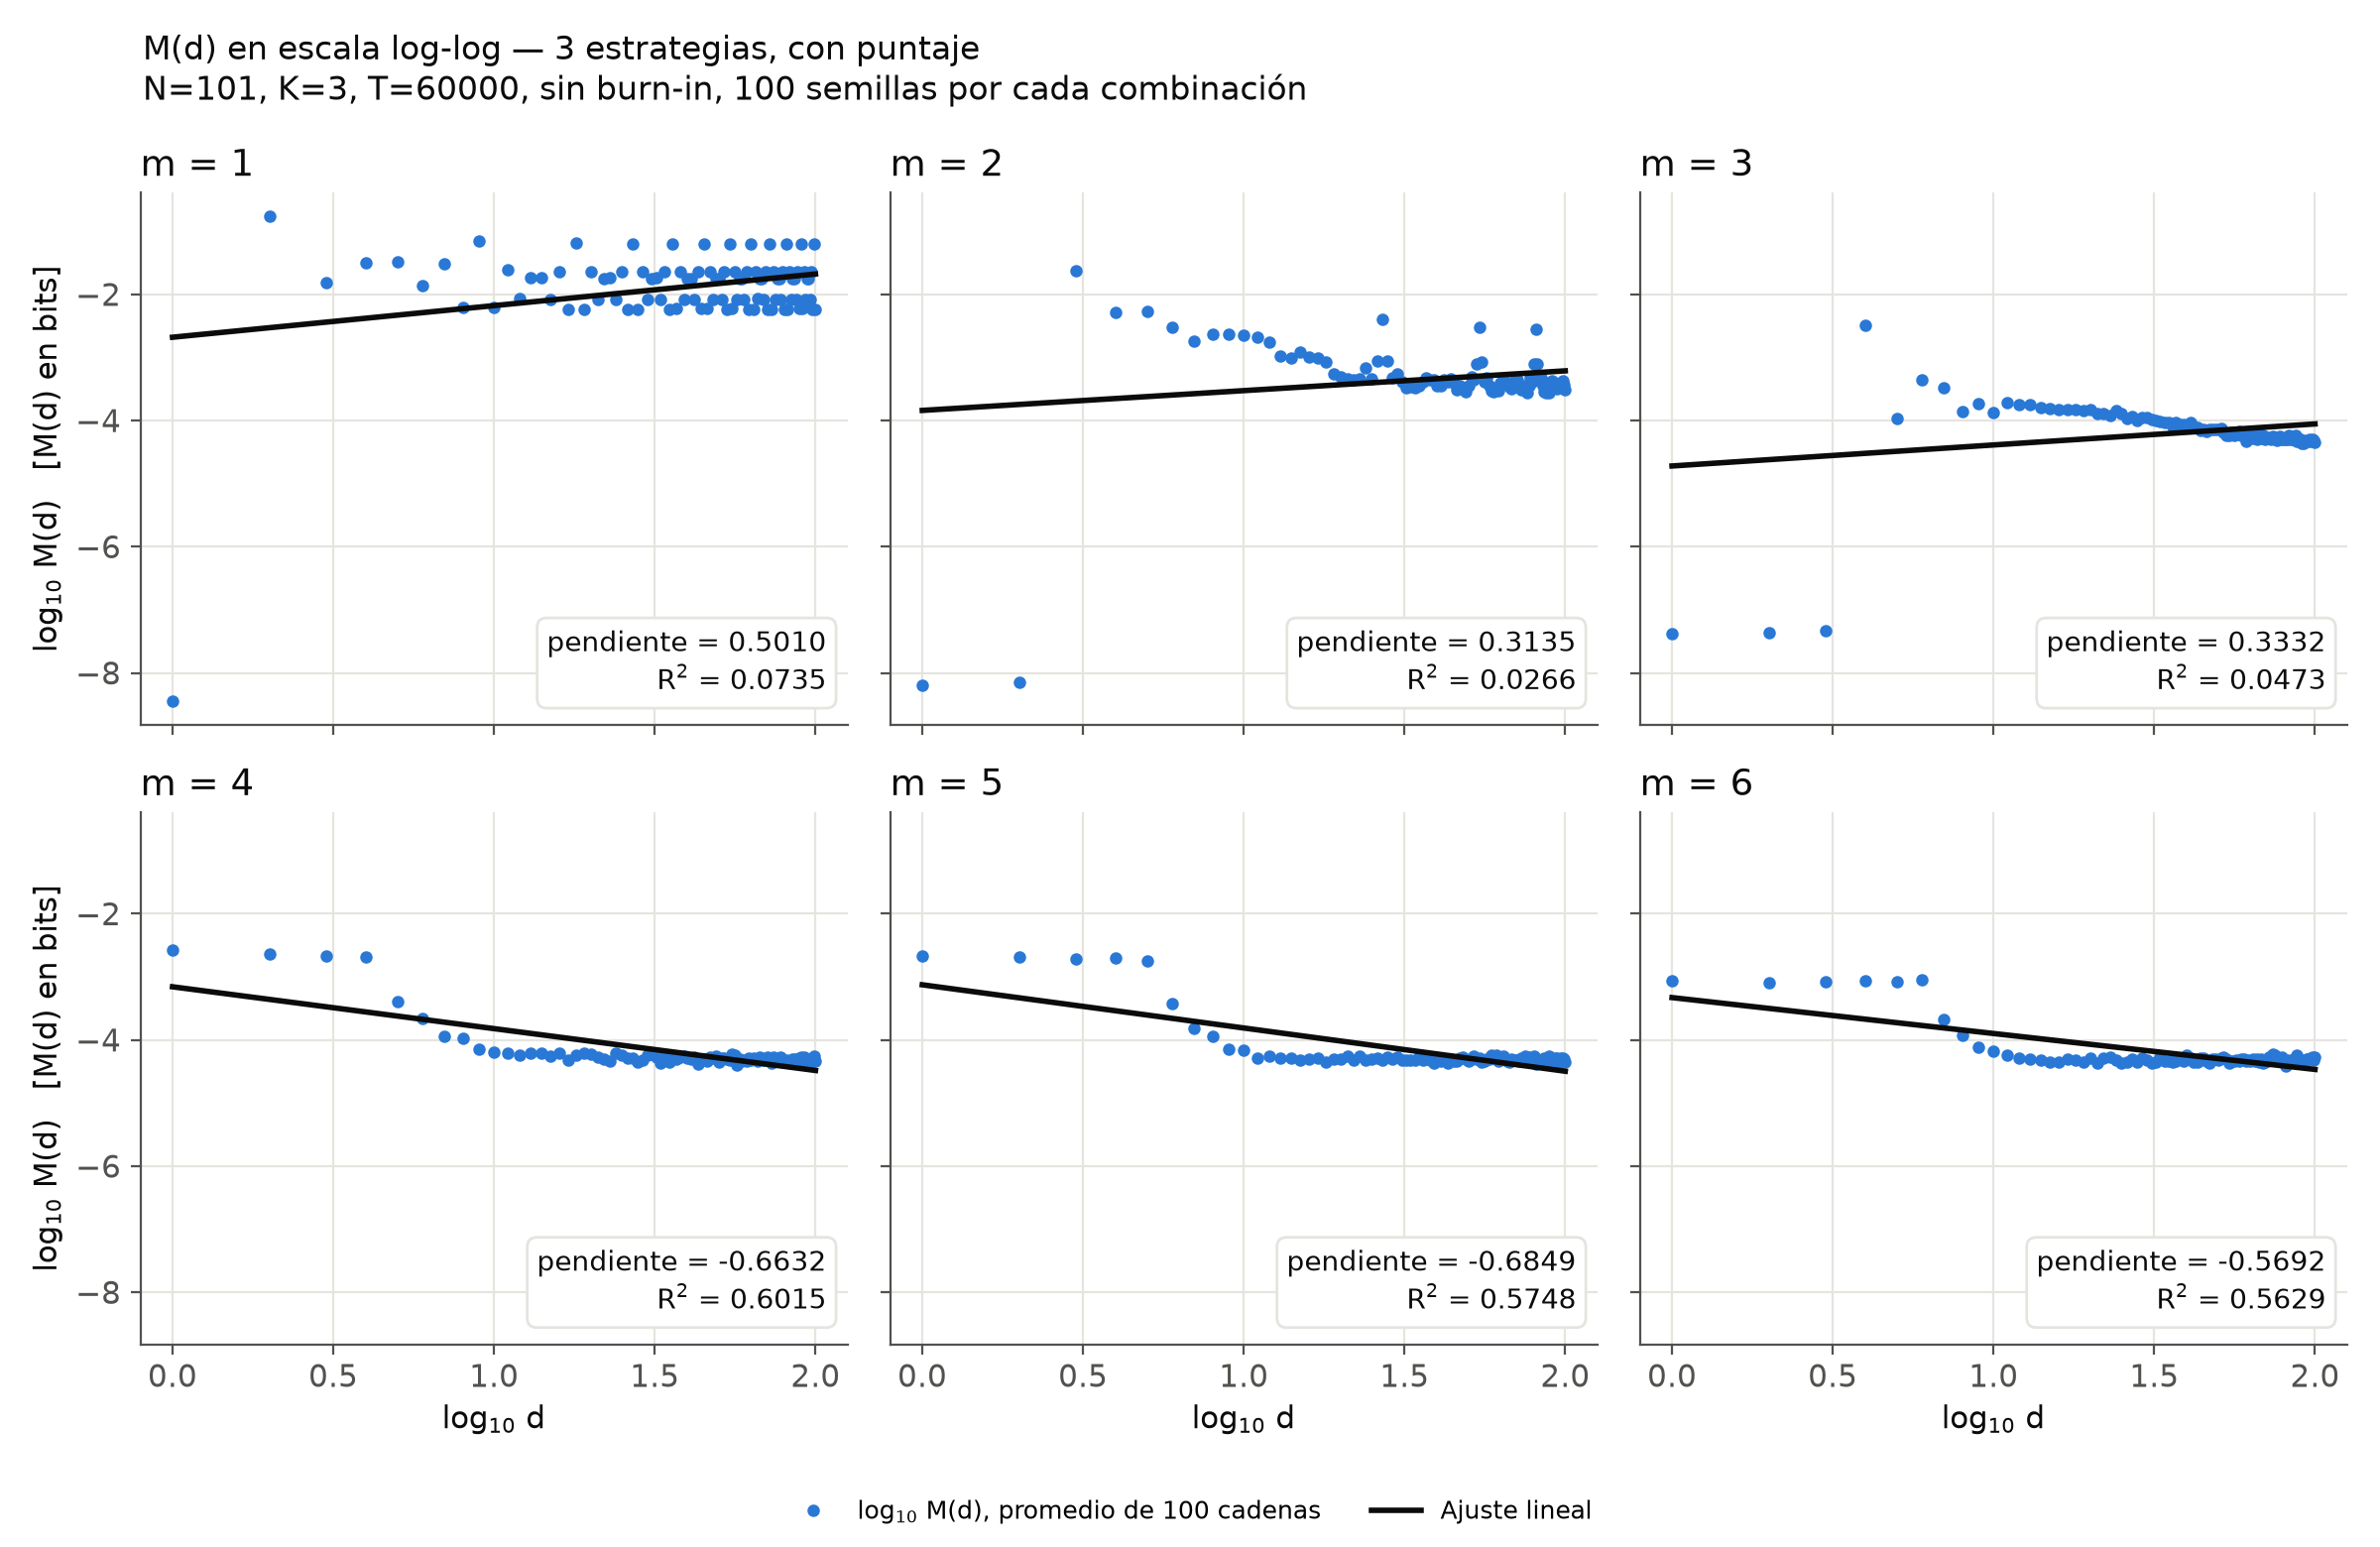
\includegraphics[width=0.92\textwidth]{figuras/Fase7_Md_loglog_con_puntaje_N101_s3_T60000_promedio.png}
\caption{Fase 7, $s=3$: $\log_{10} M(d)$ contra $\log_{10} d$, con su ajuste lineal.}
\end{figure}
\begin{figure}[H]
\centering
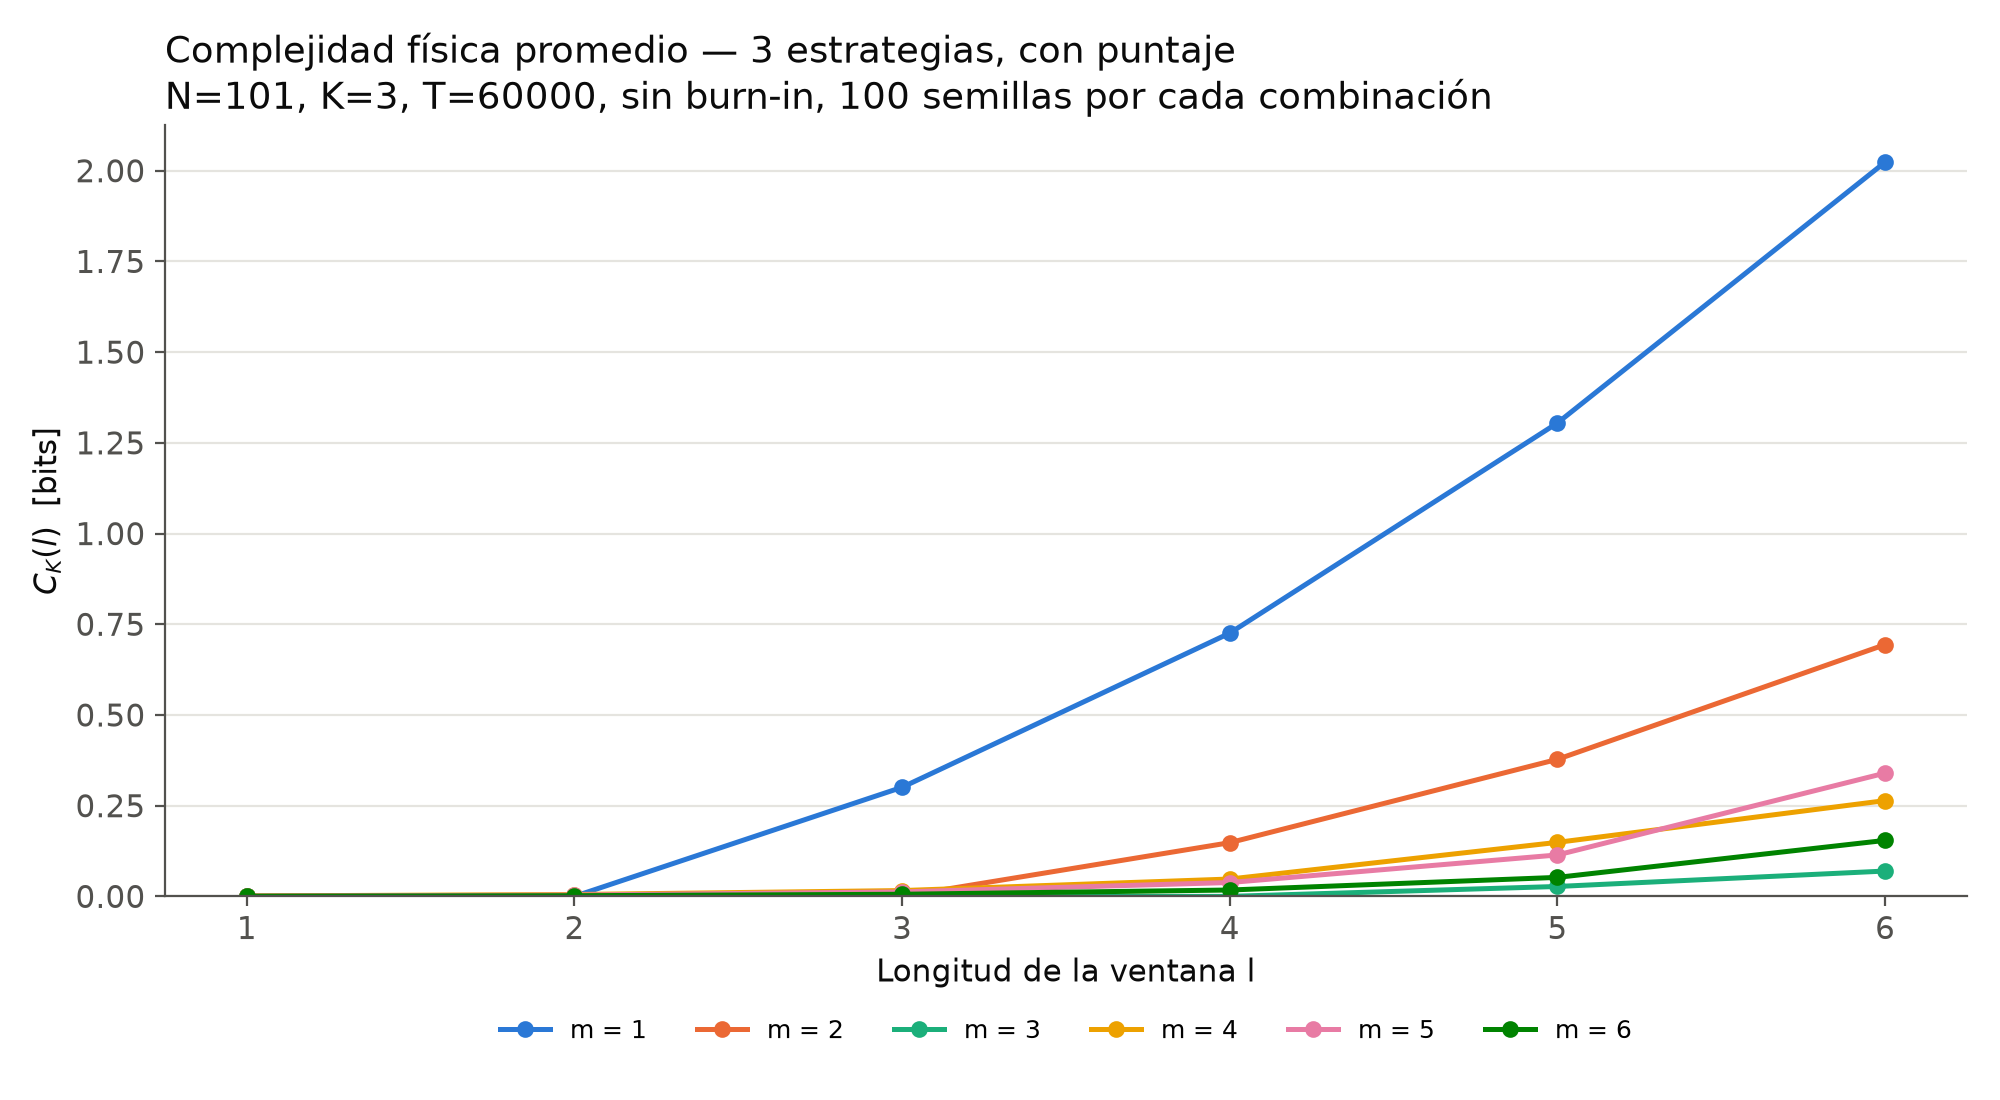
\includegraphics[width=0.92\textwidth]{figuras/Fase7_CK_con_puntaje_N101_s3_T60000_promedio.png}
\caption{Fase 7, $s=3$: $C_K(l)$ promedio contra $l$.}
\end{figure}


\section{Fase 8: juego binario}

\subsection{Validación contra la literatura}
Se calculó $\sigma^2/N$, con $\sigma^2$ la varianza temporal del número de agentes que eligen 1, y se comparó con lo esperado según Manuca \emph{et al.} y Challet, Marsili y Zecchina: que las curvas de distintos $N$ se encimen al graficarlas contra $z=2^m/N$, que tengan un mínimo cerca de $z\approx 0.3$ a $0.5$ y que tiendan a 0.25, el valor de agentes al azar, con $z$ grande. La comparación se hizo contra esos enunciados, no contra las gráficas de los artículos.

\begin{table}[H]
\centering
\footnotesize
\setlength{\tabcolsep}{3.5pt}
\caption{Fase 8, validación: $\sigma^2/N$ del juego binario ($s=2$, $T=6000$, 100 cadenas), para $N=51$, 101 y 201.}\label{tab:val}
\begin{tabular}{rrrrrrrrrr}
\toprule
$m$ & $z_{51}$ & $\sigma^2/N$ & IC 95\% & $z_{101}$ & $\sigma^2/N$ & IC 95\% & $z_{201}$ & $\sigma^2/N$ & IC 95\% \\
\midrule
1 & 0.0392 & 1.1223 & [1.0645, 1.1802] & 0.0198 & 2.1217 & [2.0214, 2.2220] & 0.0100 & 4.2661 & [4.1114, 4.4208] \\
2 & 0.0784 & 0.7029 & [0.6679, 0.7378] & 0.0396 & 1.3648 & [1.3094, 1.4202] & 0.0199 & 2.7937 & [2.6781, 2.9092] \\
3 & 0.1569 & 0.3985 & [0.3780, 0.4190] & 0.0792 & 0.8212 & [0.7915, 0.8508] & 0.0398 & 1.5900 & [1.5321, 1.6479] \\
4 & 0.3137 & 0.1122 & [0.0988, 0.1255] & 0.1584 & 0.4131 & [0.3941, 0.4321] & 0.0796 & 0.9341 & [0.9034, 0.9648] \\
5 & 0.6275 & 0.0661 & [0.0642, 0.0680] & 0.3168 & 0.1042 & [0.0950, 0.1134] & 0.1592 & 0.4214 & [0.4068, 0.4360] \\
6 & 1.2549 & 0.1062 & [0.1036, 0.1088] & 0.6337 & 0.0731 & [0.0714, 0.0748] & 0.3184 & 0.1066 & [0.1004, 0.1127] \\
7 & 2.5098 & 0.1506 & [0.1478, 0.1534] & 1.2673 & 0.1142 & [0.1123, 0.1161] & 0.6368 & 0.0856 & [0.0844, 0.0867] \\
8 & 5.0196 & 0.1889 & [0.1869, 0.1909] & 2.5347 & 0.1579 & [0.1558, 0.1599] & 1.2736 & 0.1253 & [0.1238, 0.1268] \\
9 & 10.0392 & 0.2188 & [0.2168, 0.2208] & 5.0693 & 0.1952 & [0.1934, 0.1970] & 2.5473 & 0.1689 & [0.1674, 0.1705] \\
10 & 20.0784 & 0.2339 & [0.2323, 0.2355] & 10.1386 & 0.2203 & [0.2190, 0.2216] & 5.0945 & 0.2028 & [0.2010, 0.2045] \\
\bottomrule
\end{tabular}
\end{table}


\begin{figure}[H]
\centering
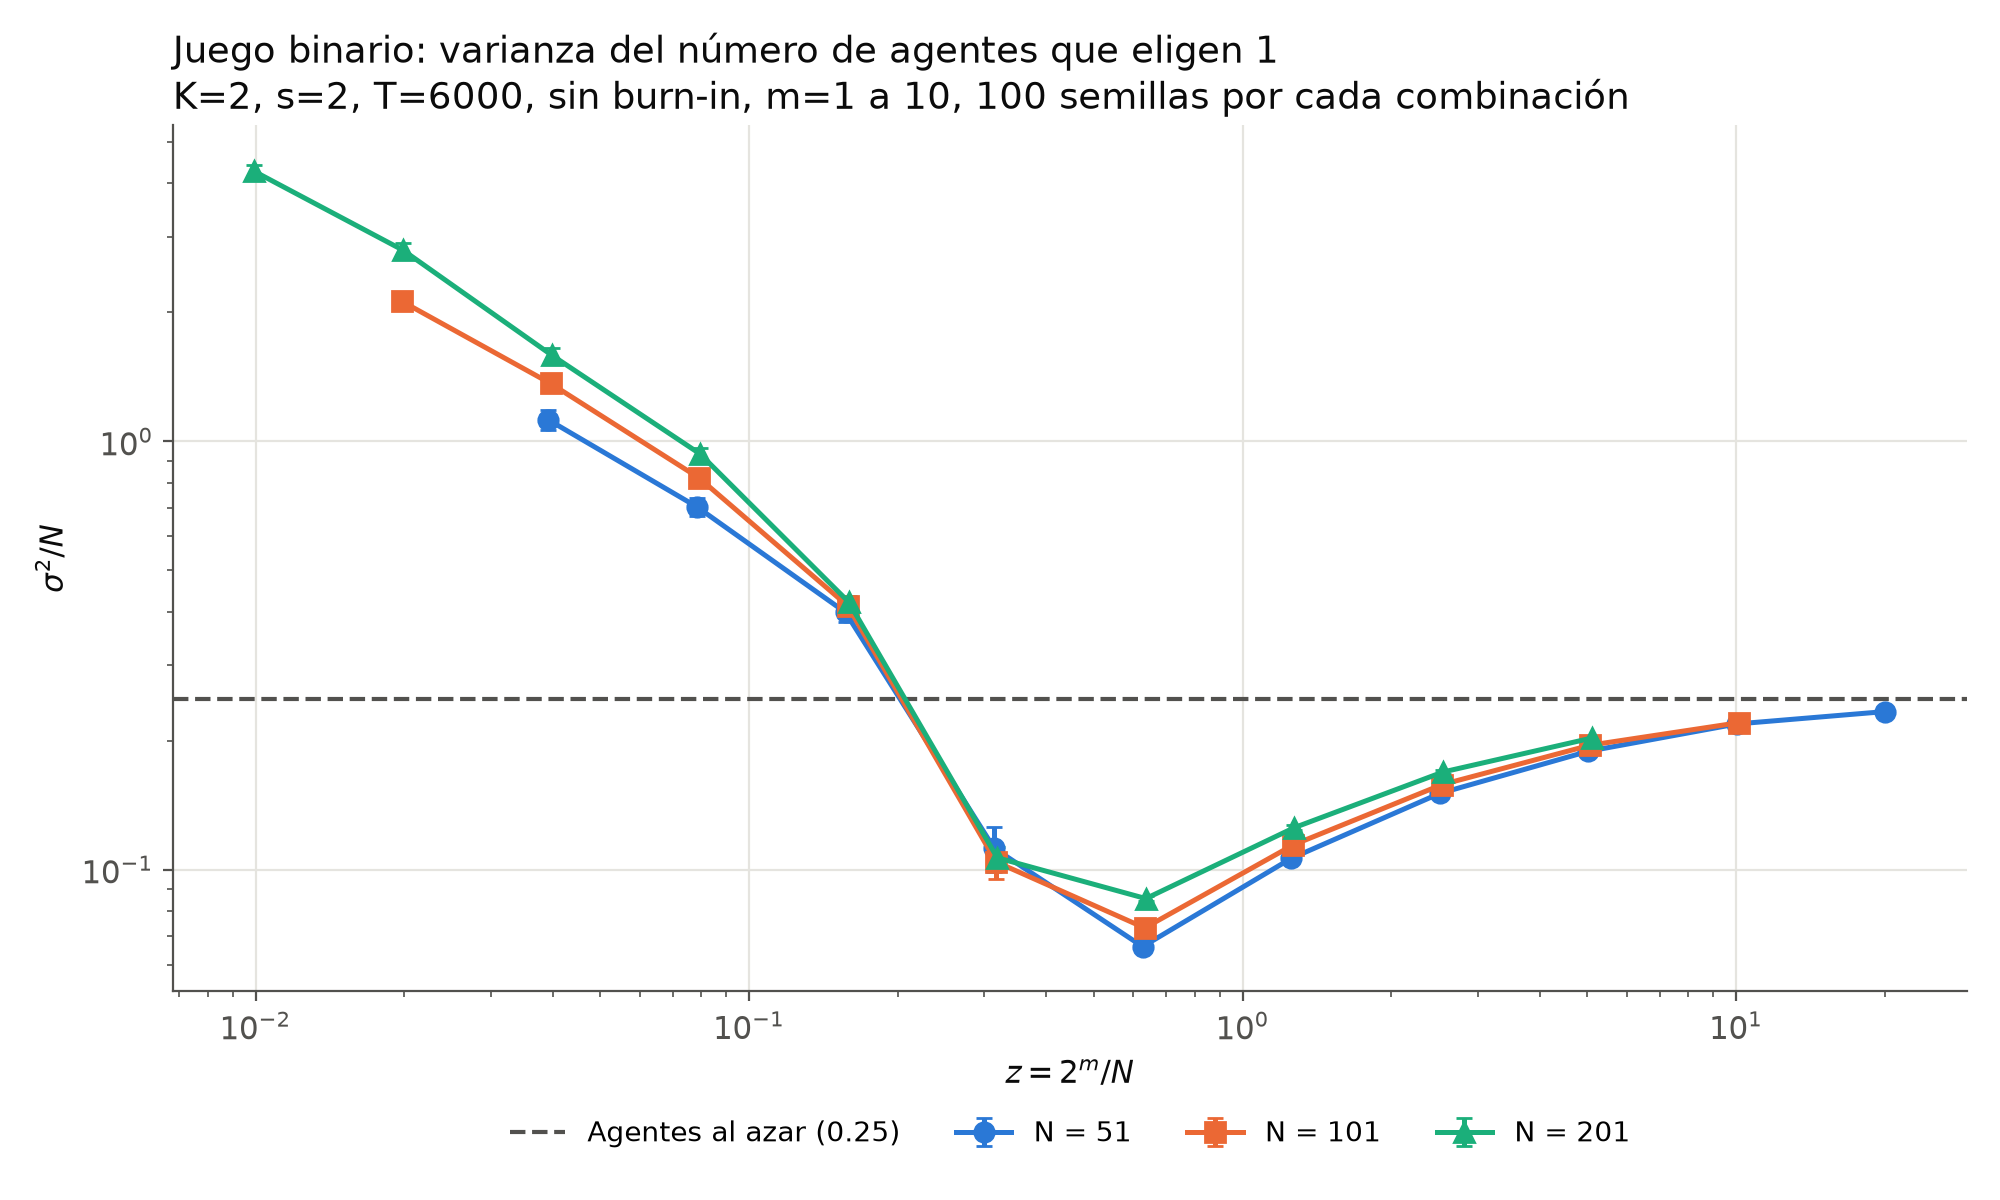
\includegraphics[width=0.9\textwidth]{figuras/Fase8_sigma2_contra_z_K2_s2_T6000_N51-101-201_m1-a-10.png}
\caption{$\sigma^2/N$ contra $z=2^m/N$ en el juego binario. La línea punteada es el valor de agentes al azar.}\label{fig:val}
\end{figure}

\textbf{Lo esperado se cumple solo en parte:}
\begin{itemize}
\item \textbf{Forma general: sí.} $\sigma^2/N$ está por encima de 0.25 con $z$ chica, cae por debajo de 0.25 y luego sube lentamente hacia 0.25.
\item \textbf{Encimado: en parte.} Las diferencias entre $N$ son de 2 a 8\,\% en $z\approx 0.16$ a $0.32$ y de 1 a 10\,\% en $z\ge 1.25$, pero de 14 a 32\,\% en $z\le 0.08$. En $z\approx 0.63$ valen 0.066, 0.073 y 0.086. En la mayoría de los puntos la diferencia supera el error estadístico.
\item \textbf{Mínimo: no confirmado.} El punto más bajo está en $z\approx 0.63$ para las tres $N$. Como $z$ se duplica con cada paso de $m$, no hay puntos entre 0.32 y 0.63, y el mínimo real podría estar en ese hueco.
\item \textbf{Límite con $z$ grande: sí, por debajo.} $\sigma^2/N$ sube hacia 0.25 sin llegar: vale 0.234 en $z\approx 20$.
\end{itemize}
No se investigó la causa de estas diferencias. Quedó pendiente, por decisión de Héctor, comprobar si influyen el arranque del juego (no hay burn-in) y la falta de puntos de $z$ cerca del mínimo.

\subsection{Barrido de memoria con $N=101$}
Se usaron los mismos $N$, $T$, $d$, $l$ y semillas que en la fase 7.

\begin{table}[H]
\centering
\footnotesize
\setlength{\tabcolsep}{3.5pt}
\caption{Fase 8, barrido de $m$ del juego binario con $s=2$ ($N=101$, $T=60000$, 100 cadenas).}\label{tab:bin2}
\begin{tabular}{rrrrrrrr}
\toprule
$m$ & $\gamma$ & $M(1)$ & $M_{\max}$ & $d_{\max}$ & $C_K(6)$ & $c_K(6)$ & IC 95\% de $c_K(6)$ \\
\midrule
1 & 0.0198 & $8.26\times10^{-10}$ & $4.62\times10^{-1}$ & 2 & $2.07\times10^{0}$ & $3.45\times10^{-1}$ & [0.32439, 0.36568] \\
2 & 0.0396 & $8.26\times10^{-10}$ & $1.88\times10^{-1}$ & 8 & $1.52\times10^{0}$ & $2.54\times10^{-1}$ & [0.23786, 0.27016] \\
3 & 0.0792 & $1.29\times10^{-9}$ & $9.07\times10^{-2}$ & 16 & $7.34\times10^{-1}$ & $1.22\times10^{-1}$ & [0.11388, 0.13088] \\
4 & 0.1584 & $2.81\times10^{-9}$ & $7.29\times10^{-3}$ & 5 & $1.05\times10^{-1}$ & $1.75\times10^{-2}$ & [0.01617, 0.01885] \\
5 & 0.3168 & $1.46\times10^{-4}$ & $2.94\times10^{-3}$ & 6 & $1.04\times10^{-2}$ & $1.73\times10^{-3}$ & [0.00078, 0.00268] \\
6 & 0.6337 & $1.38\times10^{-3}$ & $2.14\times10^{-3}$ & 6 & $1.10\times10^{-1}$ & $1.84\times10^{-2}$ & [0.01654, 0.02024] \\
7 & 1.2673 & $1.44\times10^{-3}$ & $1.75\times10^{-3}$ & 7 & $1.02\times10^{-1}$ & $1.70\times10^{-2}$ & [0.01584, 0.01823] \\
8 & 2.5347 & $1.06\times10^{-3}$ & $1.31\times10^{-3}$ & 6 & $6.97\times10^{-2}$ & $1.16\times10^{-2}$ & [0.01093, 0.01232] \\
9 & 5.0693 & $6.26\times10^{-4}$ & $9.00\times10^{-4}$ & 5 & $4.11\times10^{-2}$ & $6.85\times10^{-3}$ & [0.00636, 0.00734] \\
10 & 10.1386 & $3.40\times10^{-4}$ & $4.14\times10^{-4}$ & 9 & $2.23\times10^{-2}$ & $3.72\times10^{-3}$ & [0.00346, 0.00398] \\
\bottomrule
\end{tabular}
\end{table}
\begin{table}[H]
\centering
\footnotesize
\setlength{\tabcolsep}{3.5pt}
\caption{Fase 8, barrido de $m$ del juego binario con $s=3$ ($N=101$, $T=60000$, 100 cadenas).}\label{tab:bin3}
\begin{tabular}{rrrrrrrr}
\toprule
$m$ & $\gamma$ & $M(1)$ & $M_{\max}$ & $d_{\max}$ & $C_K(6)$ & $c_K(6)$ & IC 95\% de $c_K(6)$ \\
\midrule
1 & 0.0198 & $7.45\times10^{-10}$ & $3.63\times10^{-1}$ & 2 & $1.67\times10^{0}$ & $2.79\times10^{-1}$ & [0.26118, 0.29712] \\
2 & 0.0396 & $8.26\times10^{-10}$ & $1.09\times10^{-1}$ & 8 & $1.22\times10^{0}$ & $2.03\times10^{-1}$ & [0.18990, 0.21700] \\
3 & 0.0792 & $1.18\times10^{-9}$ & $7.20\times10^{-2}$ & 16 & $6.42\times10^{-1}$ & $1.07\times10^{-1}$ & [0.09821, 0.11579] \\
4 & 0.1584 & $1.47\times10^{-9}$ & $9.73\times10^{-3}$ & 5 & $1.41\times10^{-1}$ & $2.34\times10^{-2}$ & [0.02161, 0.02523] \\
5 & 0.3168 & $3.95\times10^{-9}$ & $4.94\times10^{-3}$ & 6 & $3.00\times10^{-7}$ & $5.00\times10^{-8}$ & [0.00000, 0.00000] \\
6 & 0.6337 & $9.54\times10^{-8}$ & $2.69\times10^{-4}$ & 7 & $5.42\times10^{-5}$ & $9.04\times10^{-6}$ & [-0.00001, 0.00003] \\
7 & 1.2673 & $3.04\times10^{-4}$ & $3.58\times10^{-4}$ & 6 & $1.73\times10^{-2}$ & $2.89\times10^{-3}$ & [0.00263, 0.00315] \\
8 & 2.5347 & $2.81\times10^{-4}$ & $4.11\times10^{-4}$ & 2 & $2.43\times10^{-2}$ & $4.05\times10^{-3}$ & [0.00380, 0.00430] \\
9 & 5.0693 & $2.56\times10^{-4}$ & $3.87\times10^{-4}$ & 5 & $1.71\times10^{-2}$ & $2.85\times10^{-3}$ & [0.00268, 0.00303] \\
10 & 10.1386 & $1.71\times10^{-4}$ & $2.16\times10^{-4}$ & 5 & $1.09\times10^{-2}$ & $1.82\times10^{-3}$ & [0.00171, 0.00194] \\
\bottomrule
\end{tabular}
\end{table}


\subsubsection*{Gráficas con $s=2$}
\begin{figure}[H]
\centering
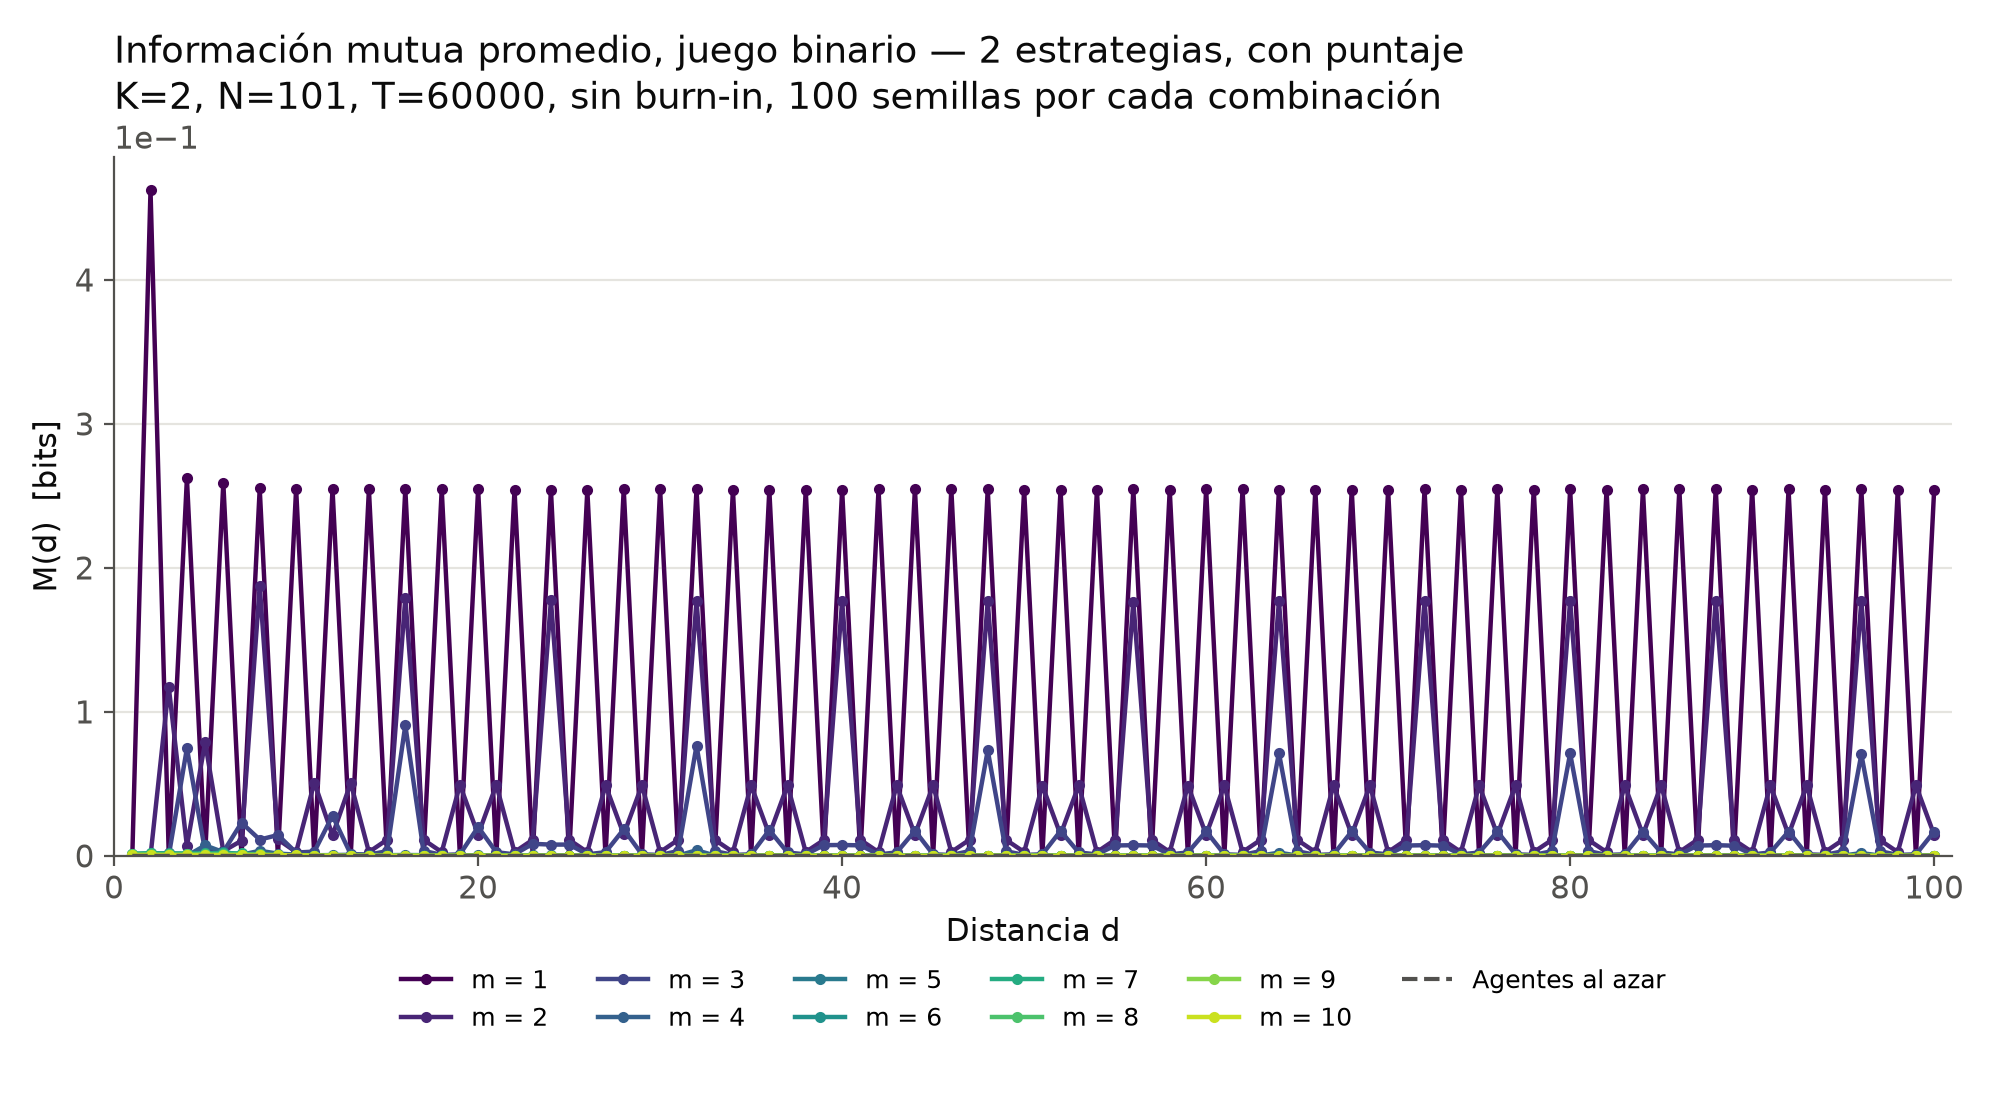
\includegraphics[width=0.92\textwidth]{figuras/Fase8_binario_Md_con_puntaje_N101_s2_T60000_promedio.png}
\caption{Juego binario, $s=2$: $M(d)$ promedio, una curva por $m$, con la referencia de agentes al azar.}
\end{figure}
\begin{figure}[H]
\centering
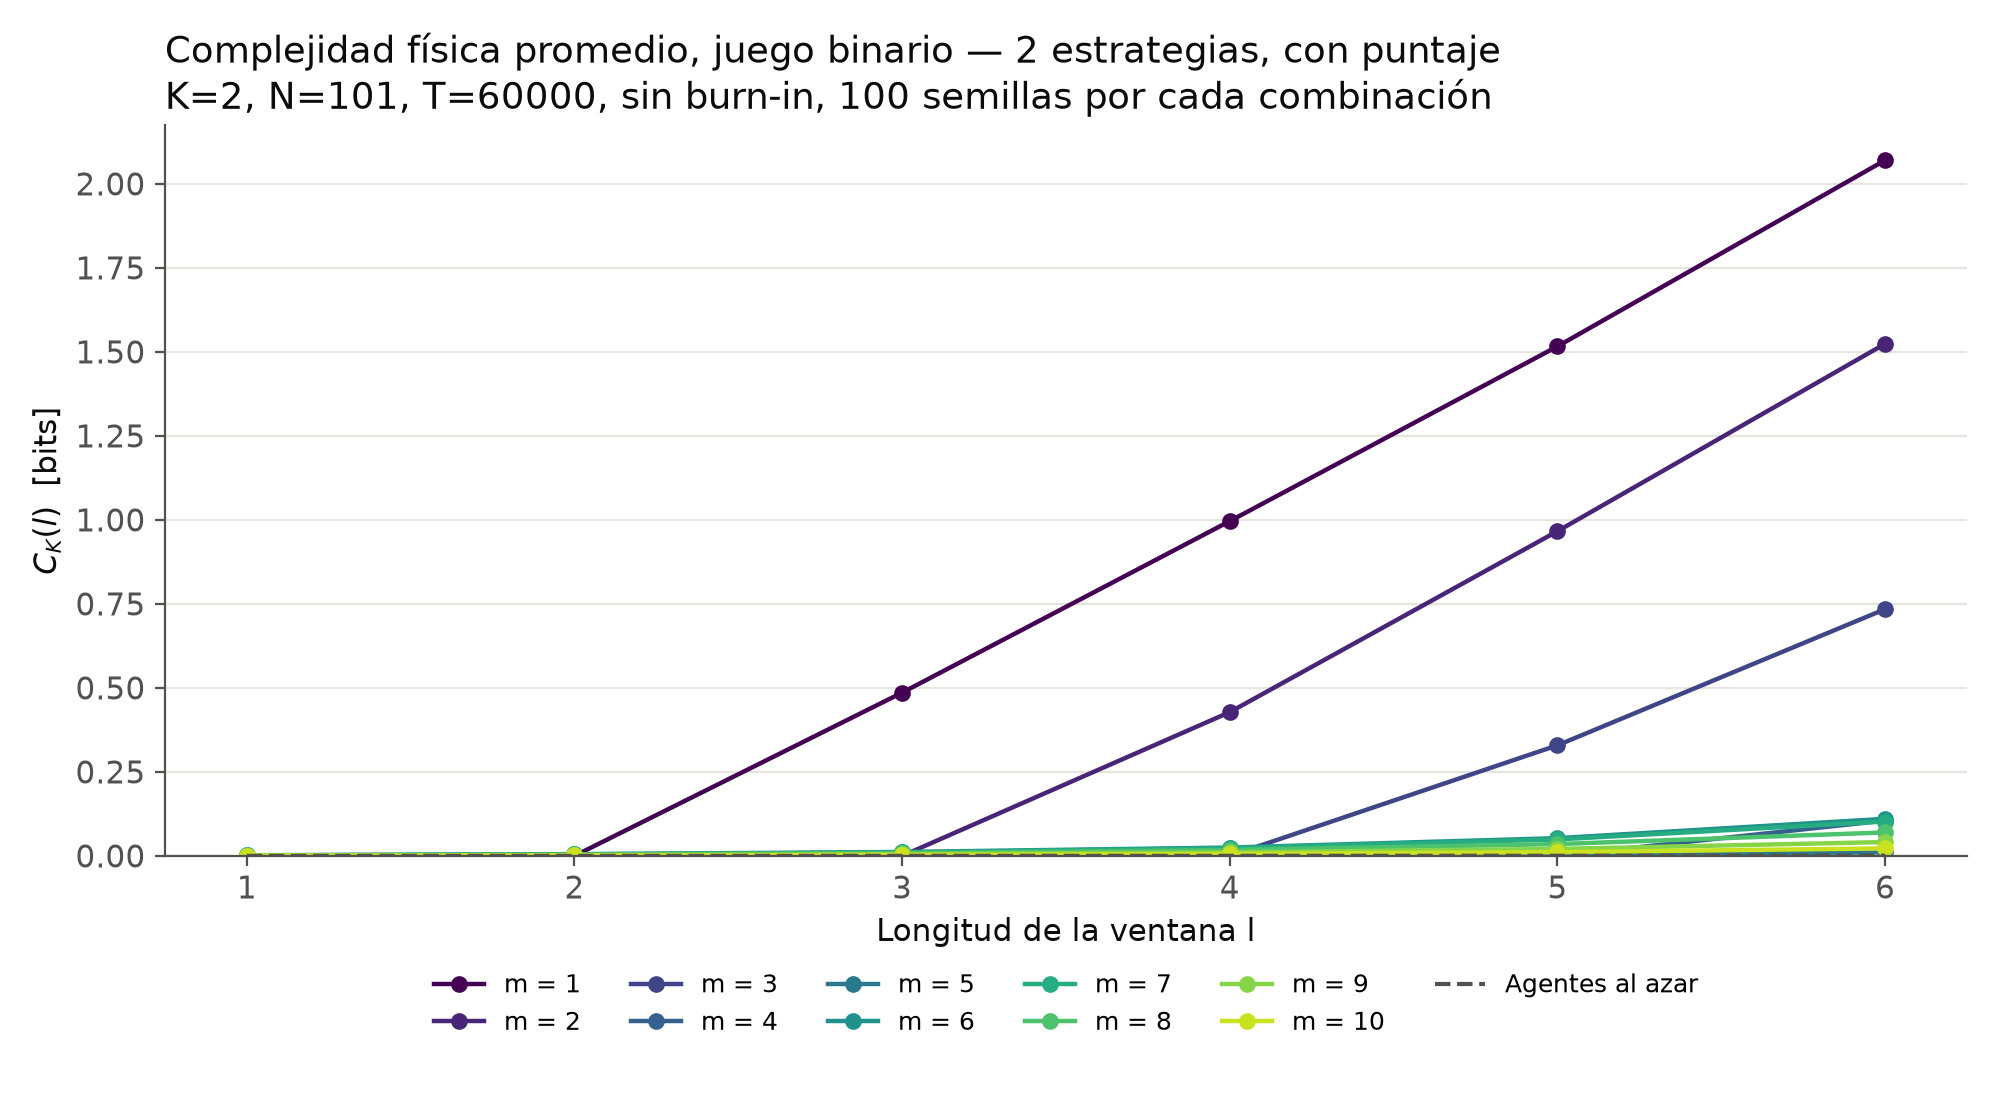
\includegraphics[width=0.92\textwidth]{figuras/Fase8_binario_CK_con_puntaje_N101_s2_T60000_promedio.png}
\caption{Juego binario, $s=2$: $C_K(l)$ promedio contra $l$.}
\end{figure}

\subsubsection*{Gráficas con $s=3$}
\begin{figure}[H]
\centering
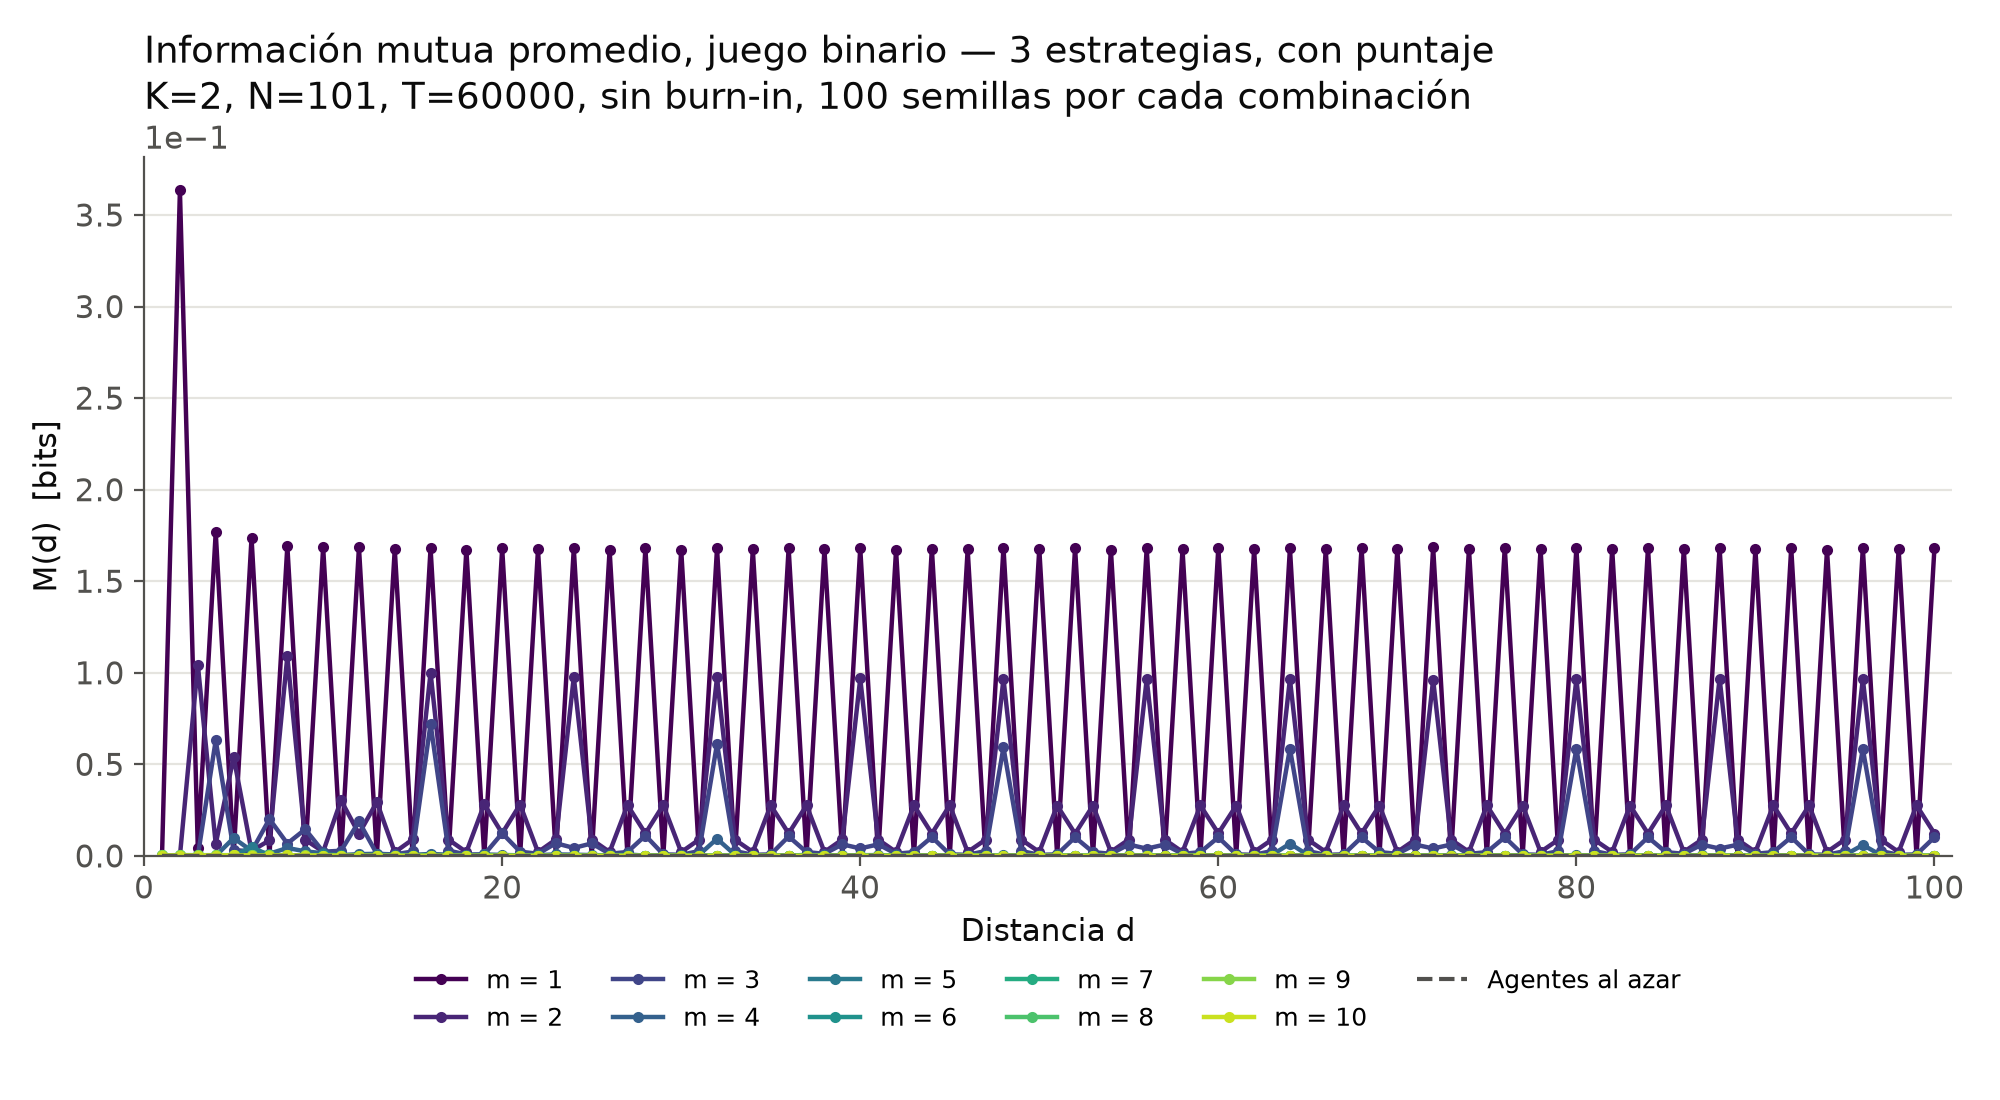
\includegraphics[width=0.92\textwidth]{figuras/Fase8_binario_Md_con_puntaje_N101_s3_T60000_promedio.png}
\caption{Juego binario, $s=3$: $M(d)$ promedio, una curva por $m$, con la referencia de agentes al azar.}
\end{figure}
\begin{figure}[H]
\centering
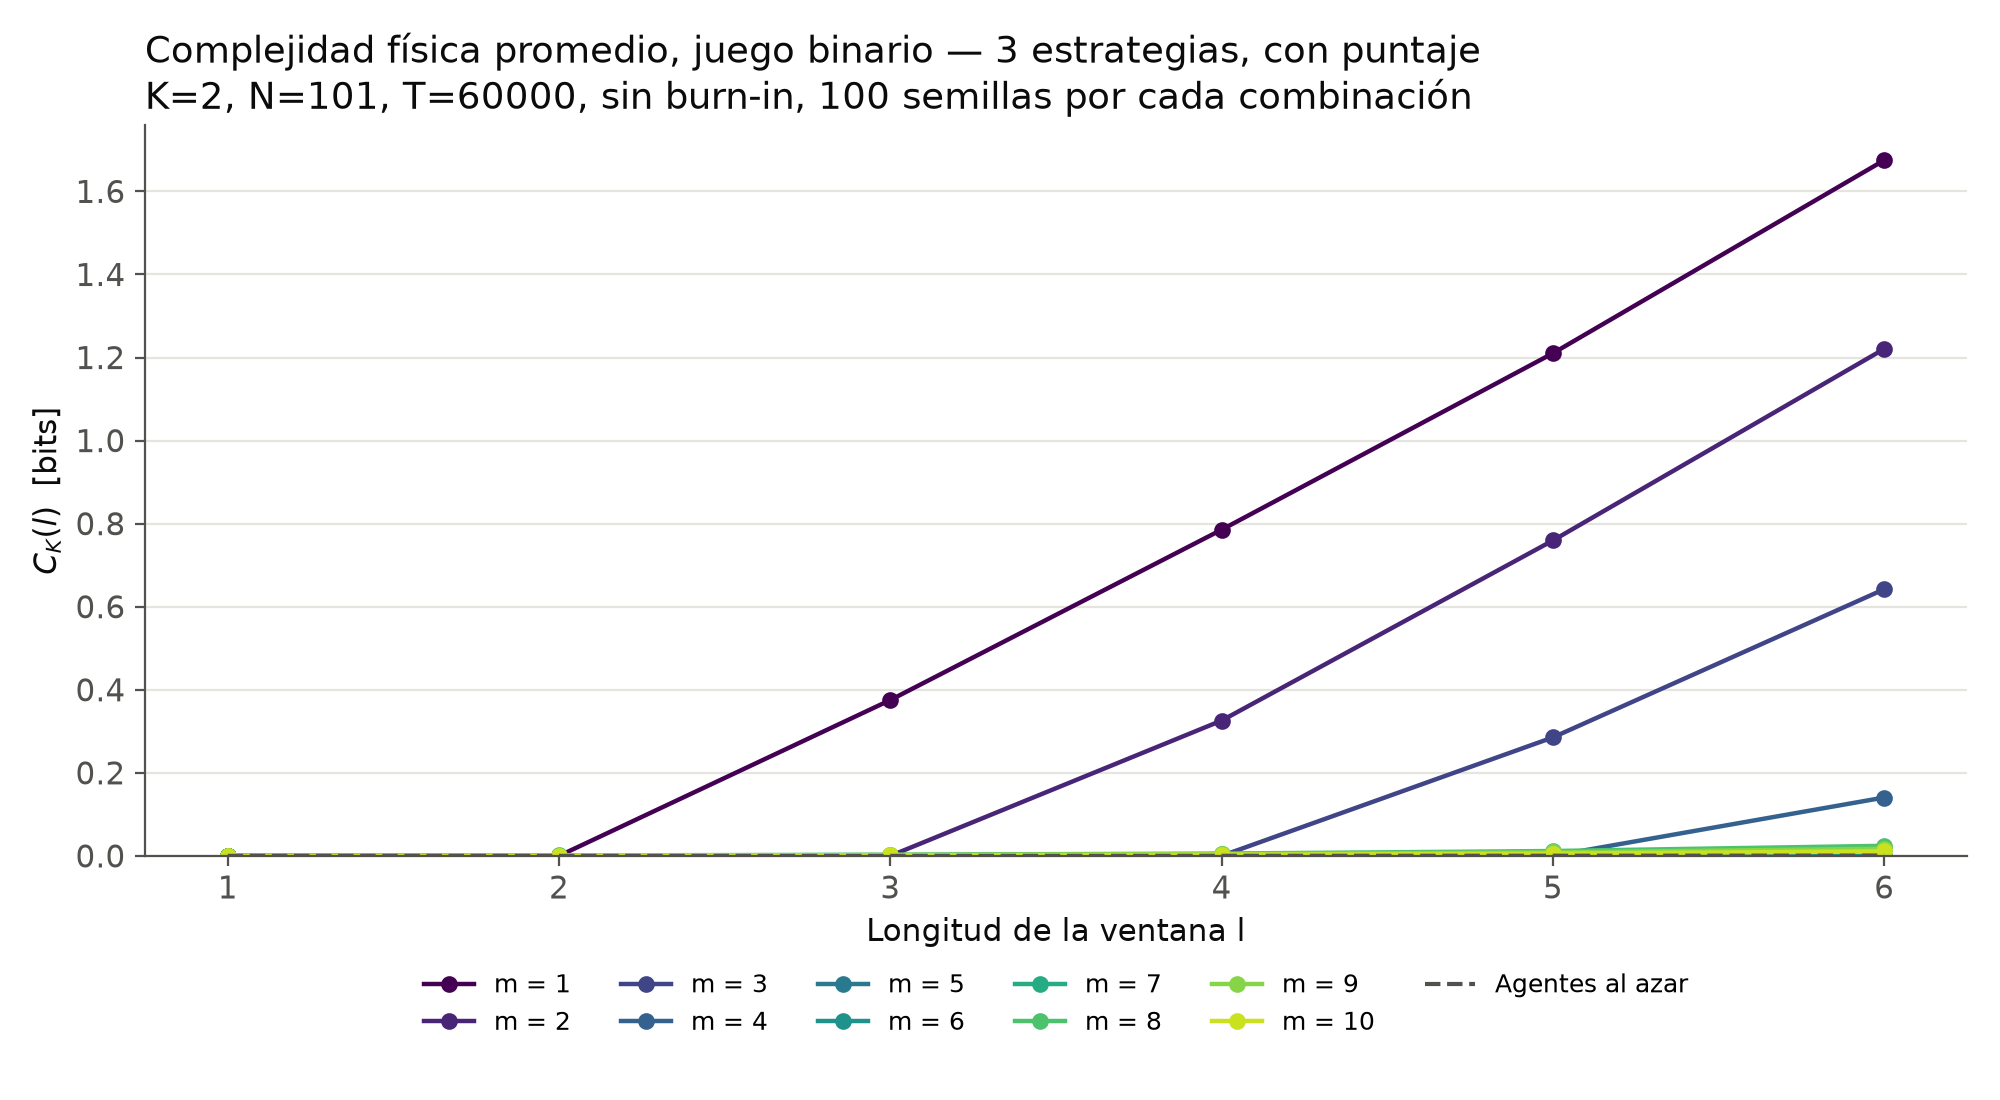
\includegraphics[width=0.92\textwidth]{figuras/Fase8_binario_CK_con_puntaje_N101_s3_T60000_promedio.png}
\caption{Juego binario, $s=3$: $C_K(l)$ promedio contra $l$.}
\end{figure}


\subsubsection*{Observaciones del binario}
\begin{itemize}
\item \textbf{Con $s=2$ la forma de $M(d)$ cambia entre $m=4$ y $m=6$, y $m=5$ es intermedio.} Hasta $m=4$, $M(d)\sim 10^{-9}$ para $d\le m$ y el máximo aparece en $d=m+1$ o en un múltiplo de $2^{m+1}$. Con $m=5$, $M(1)$ es de $1.5\times10^{-4}$ con un intervalo muy ancho (de $9.5\times10^{-6}$ a $2.8\times10^{-4}$), y sigue habiendo un pico en $d=6$. Desde $m=6$, $M(d)$ es casi plana de $d=1$ a $d\approx m$, y luego cae.
\item \textbf{Con $s=3$ la forma cambia entre $m=6$ y $m=7$.} Hasta $m=6$, $M(d)$ es del orden de $10^{-9}$ a $10^{-6}$ para $d\le m$ y tiene un pico en $d=m+1$. Desde $m=7$ se vuelve casi plana hasta $d\approx m$.
\item \textbf{Periodicidad.} Para $m=2$, 3 y 4 hay picos en múltiplos de $2^{m+1}$ (8, 16 y 32), con ambas $s$. Para $m=1$ los picos están en todas las distancias pares. Con $m\ge 5$ no se observan.
\item \textbf{Complejidad.} Antes del cambio $C_K(l)$ es prácticamente cero hasta $l=m+1$. Después, es distinta de cero en todo $l$.
\item \textbf{$M(1)$ antes del cambio} es mucho menor que la referencia de agentes al azar ($\sim10^{-9}$ contra $1.2\times10^{-5}$), en los dos juegos.
\end{itemize}

\subsection{Referencia de agentes al azar}
\begin{table}[H]
\centering
\footnotesize
\setlength{\tabcolsep}{3.5pt}
\caption{Referencia de agentes que eligen al azar ($N=101$, $T=60000$, 100 cadenas).}\label{tab:ref}
\begin{tabular}{rrrrr}
\toprule
$K$ & $M(1)$ & $M(1)/\log_2 K$ & $C_K(6)$ & $c_K(6)$ \\
\midrule
2 & $1.21\times10^{-5}$ & $1.21\times10^{-5}$ & $7.71\times10^{-4}$ & $1.28\times10^{-4}$ \\
3 & $5.25\times10^{-5}$ & $3.31\times10^{-5}$ & $8.83\times10^{-3}$ & $9.28\times10^{-4}$ \\
\bottomrule
\end{tabular}
\end{table}

Cada juego se compara con la referencia de su propio alfabeto. Los valores de $M(1)$ son consistentes con el sesgo de una cadena finita sin correlación, $(K-1)^2/(2\,n\ln 2)$, que vale $1.2\times10^{-5}$ bits para $K=2$ y $4.8\times10^{-5}$ bits para $K=3$ con $T=60000$.

\subsection{Comparación entre los dos juegos}

\subsubsection*{Con $s=2$}
\begin{figure}[H]
\centering
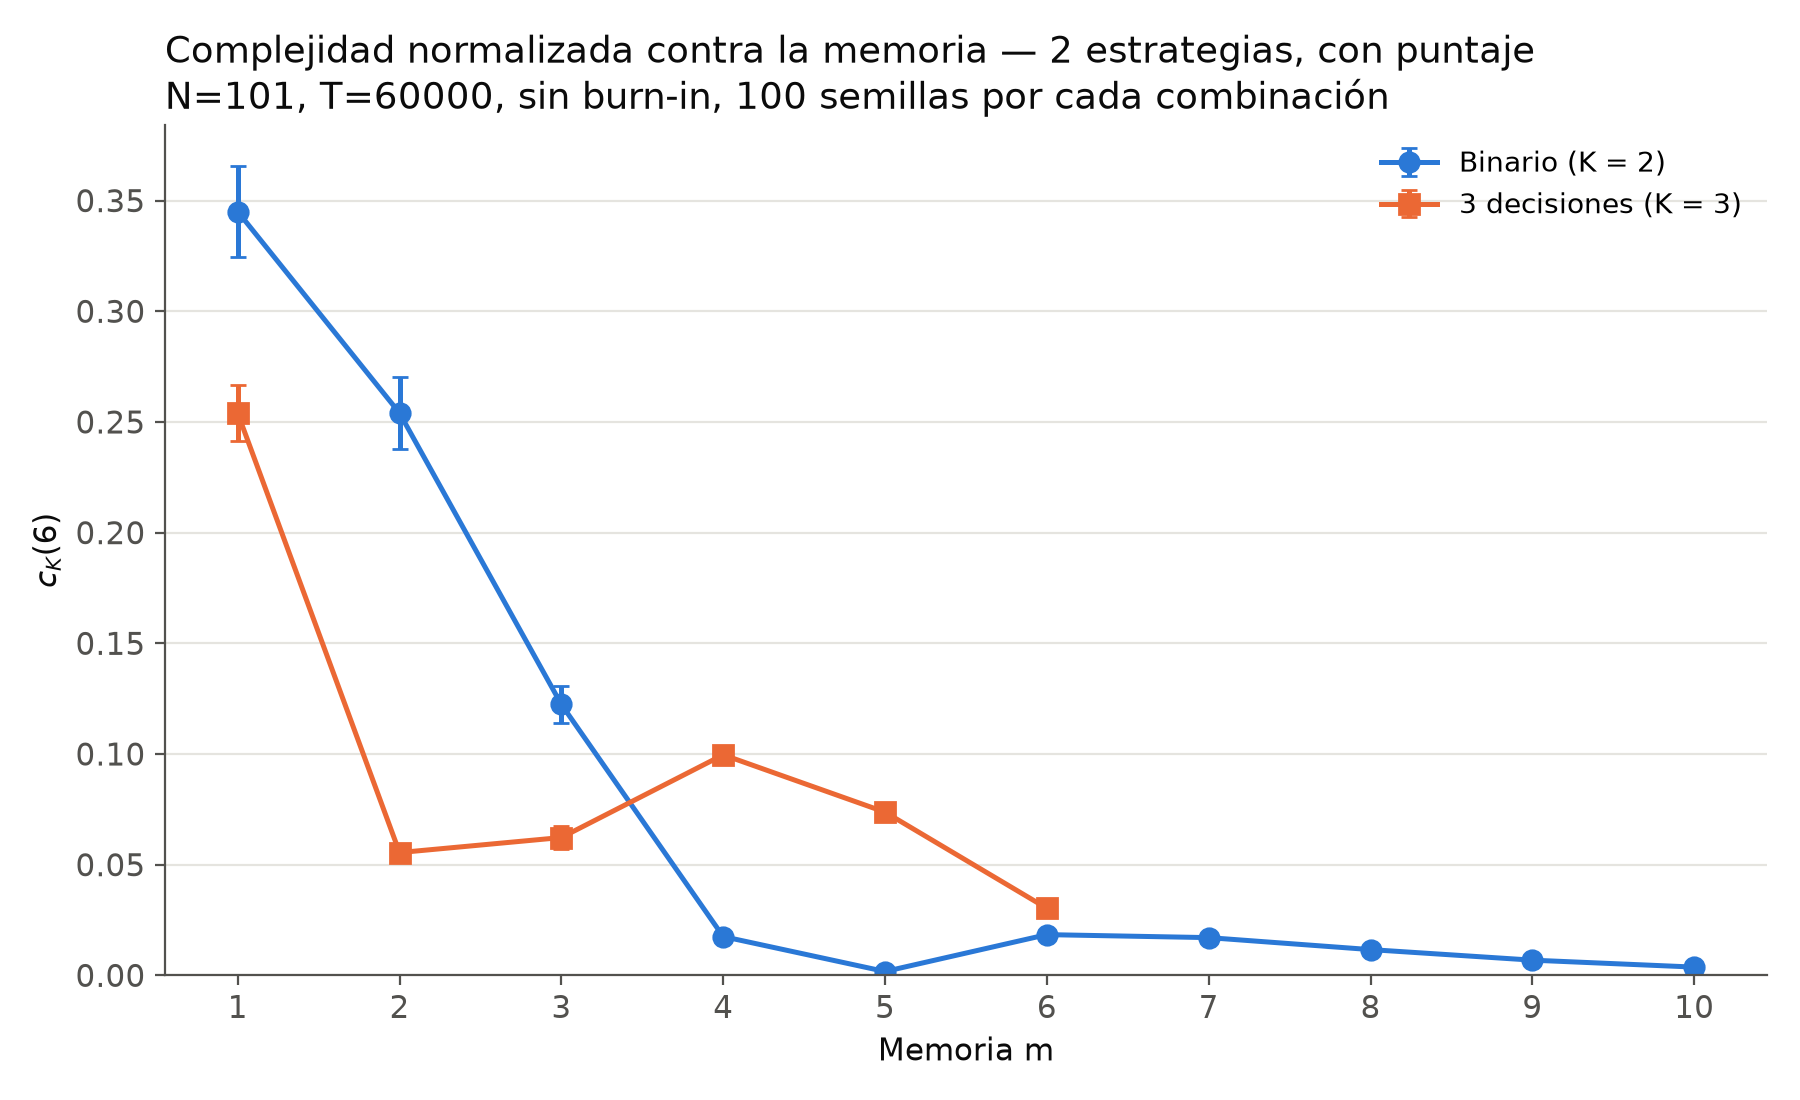
\includegraphics[width=0.8\textwidth]{figuras/Fase8_comparacion_c6_contra_m_con_puntaje_N101_s2_T60000.png}
\caption{Comparación, $s=2$: $c_K(6)$ contra $m$, con intervalo de confianza del 95\%.}
\end{figure}
\begin{figure}[H]
\centering
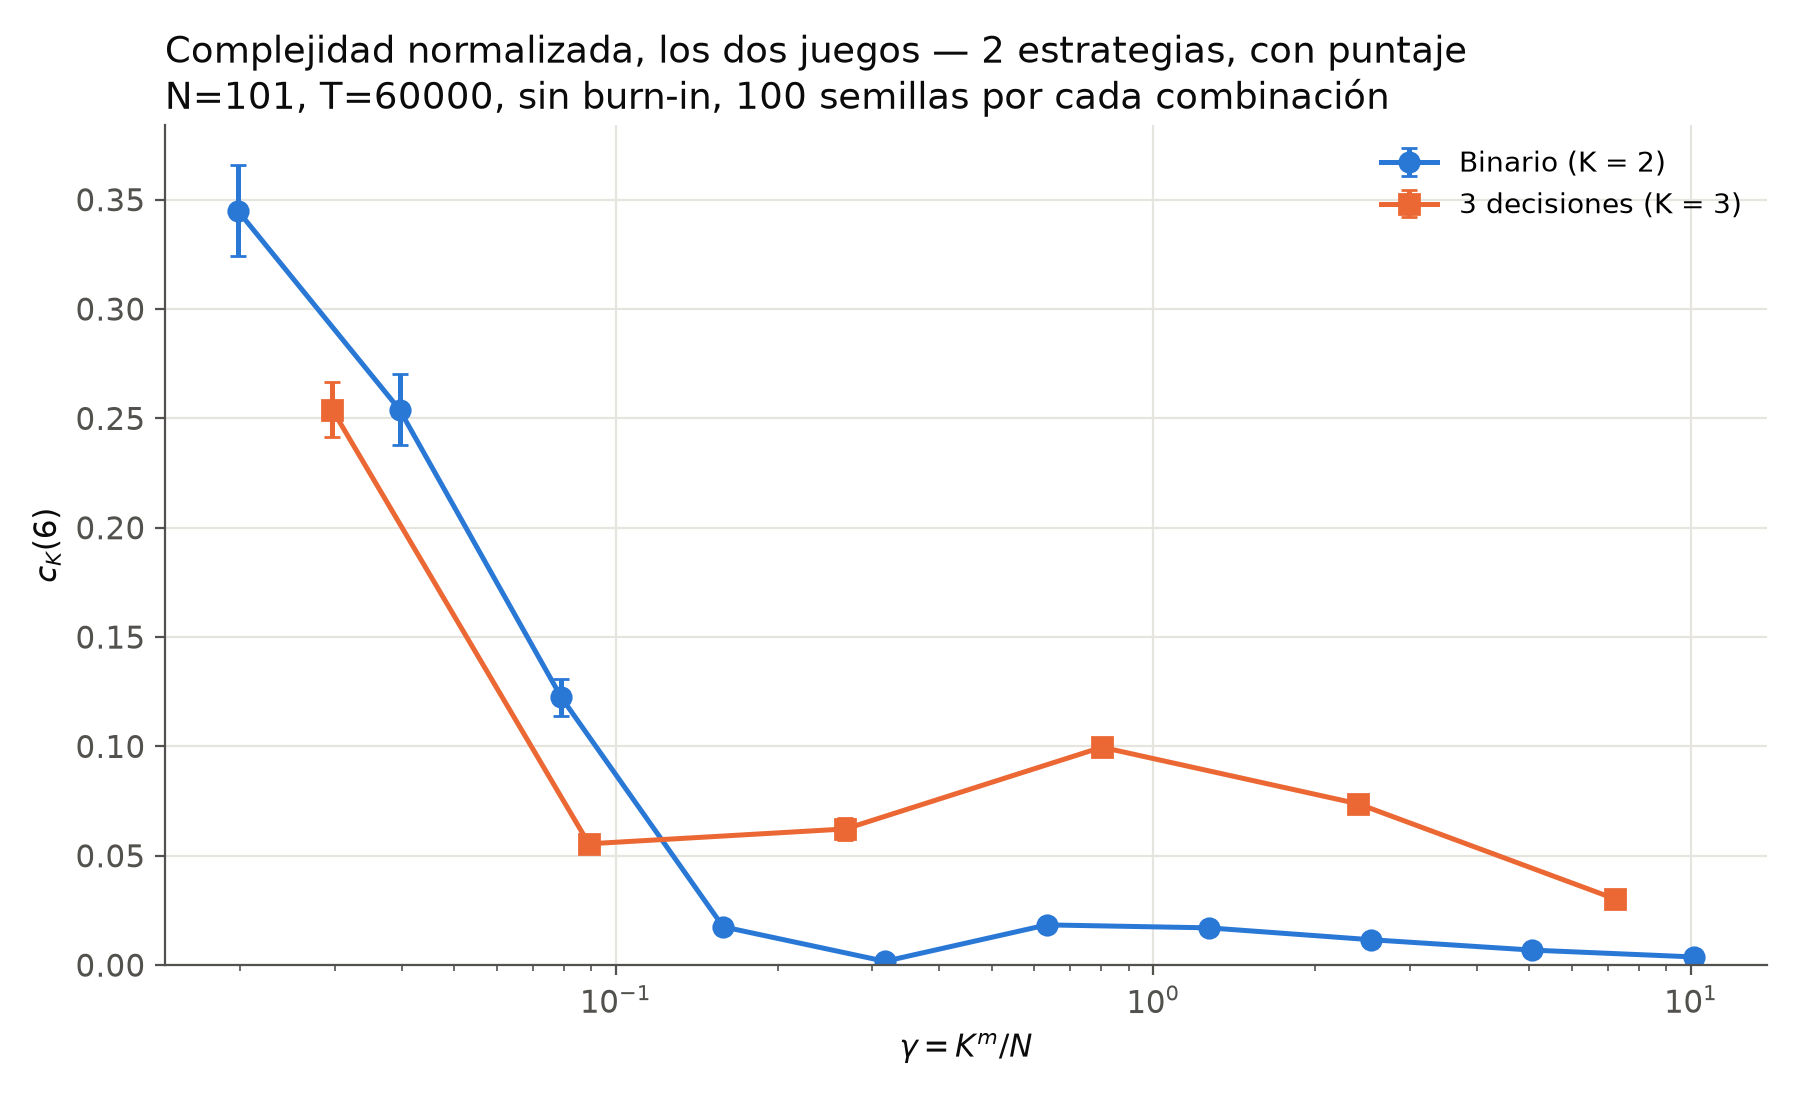
\includegraphics[width=0.8\textwidth]{figuras/Fase8_comparacion_c6_contra_gamma_con_puntaje_N101_s2_T60000.png}
\caption{Comparación, $s=2$: $c_K(6)$ contra $\gamma=K^m/N$.}
\end{figure}
\begin{figure}[H]
\centering
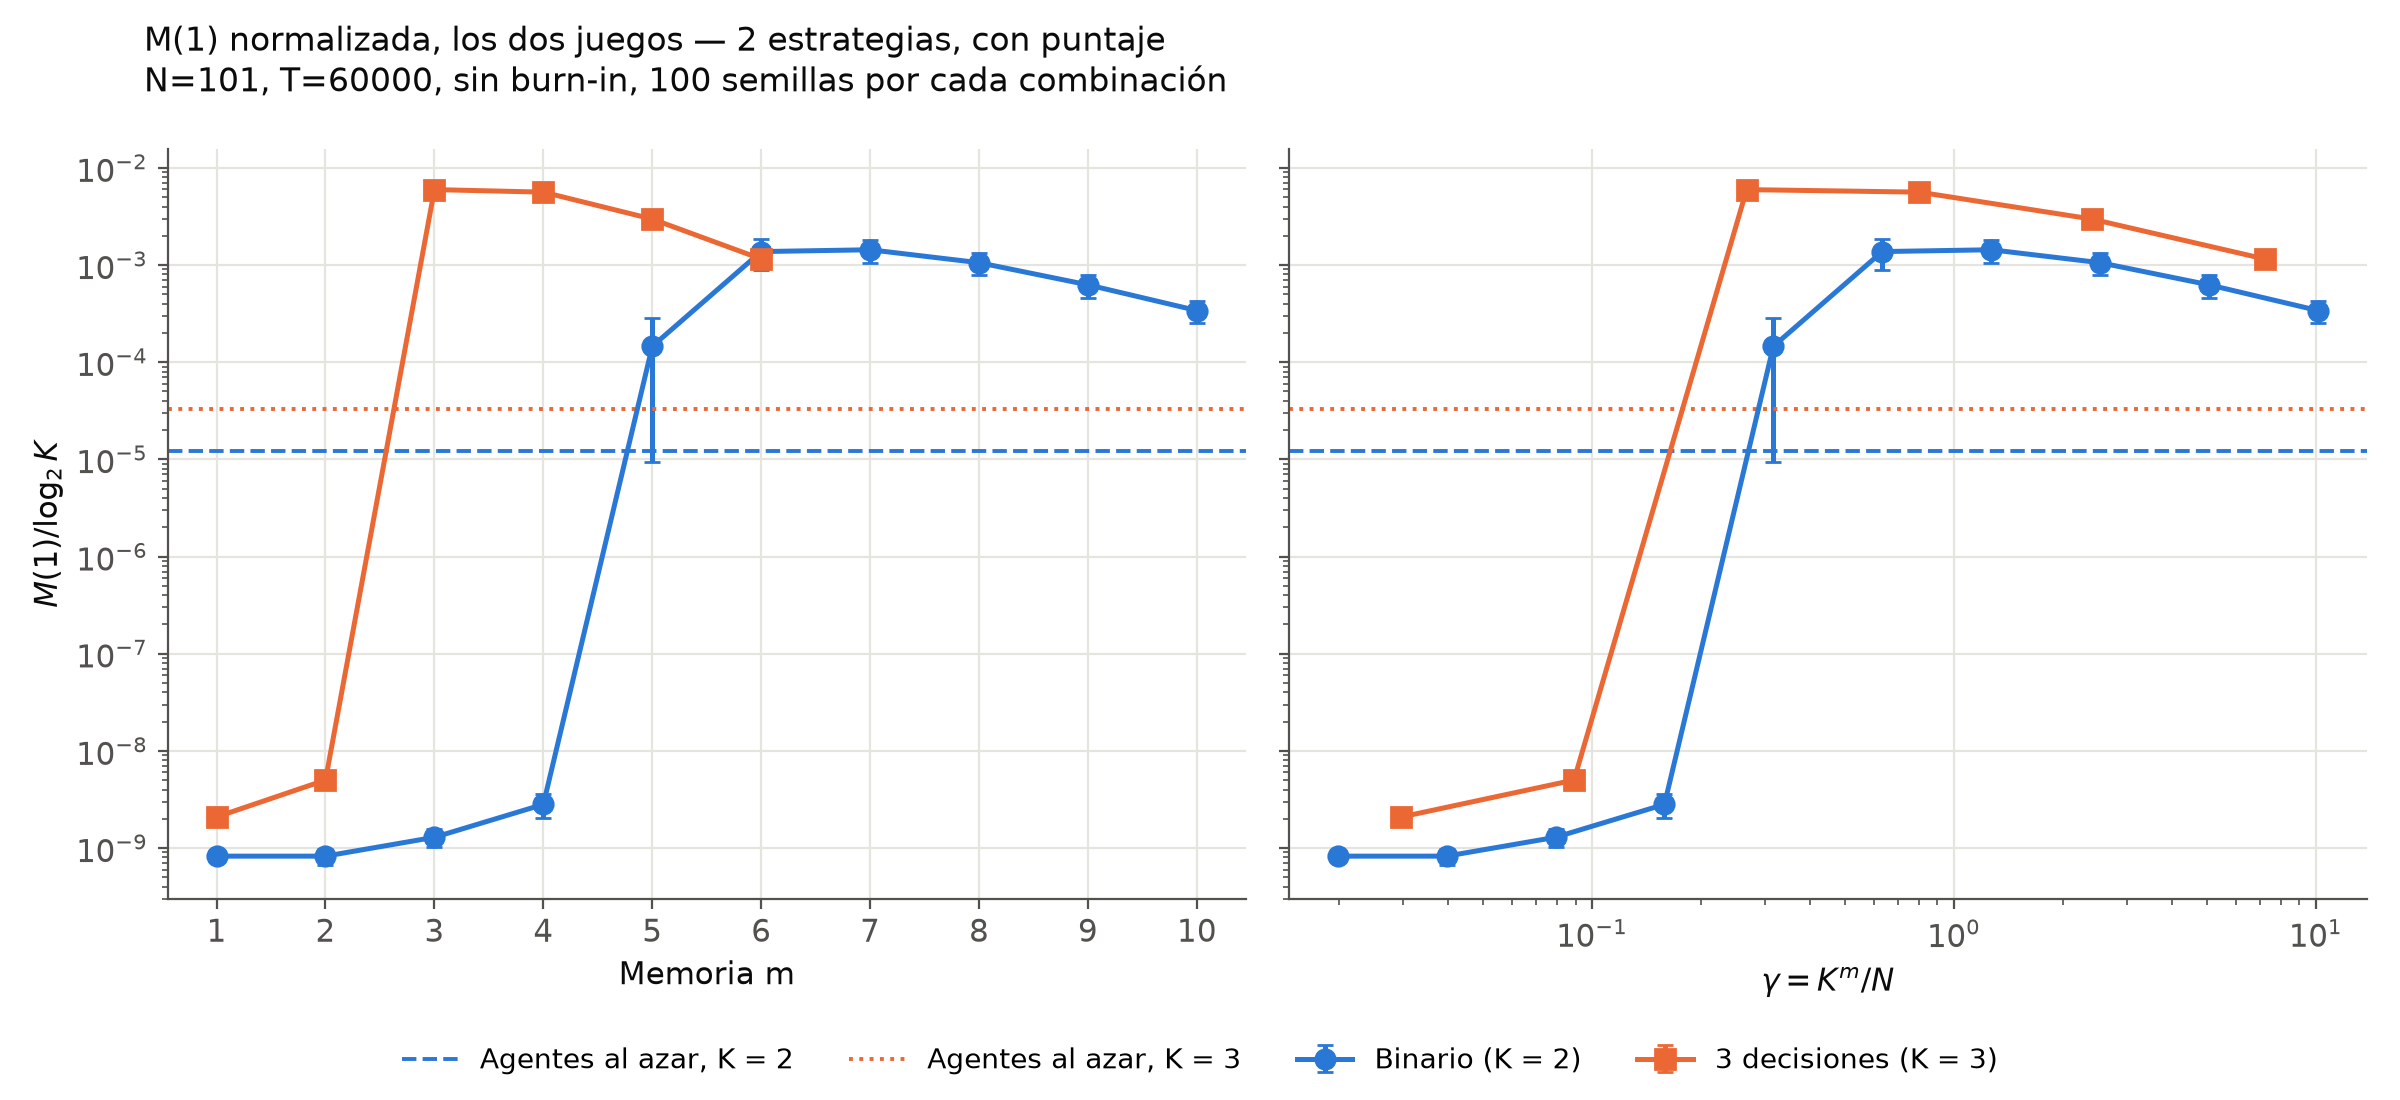
\includegraphics[width=0.92\textwidth]{figuras/Fase8_comparacion_M1_con_puntaje_N101_s2_T60000.png}
\caption{Comparación, $s=2$: $M(1)/\log_2 K$ contra $m$ y contra $\gamma$, con la referencia normalizada de cada juego.}
\end{figure}

\subsubsection*{Con $s=3$}
\begin{figure}[H]
\centering
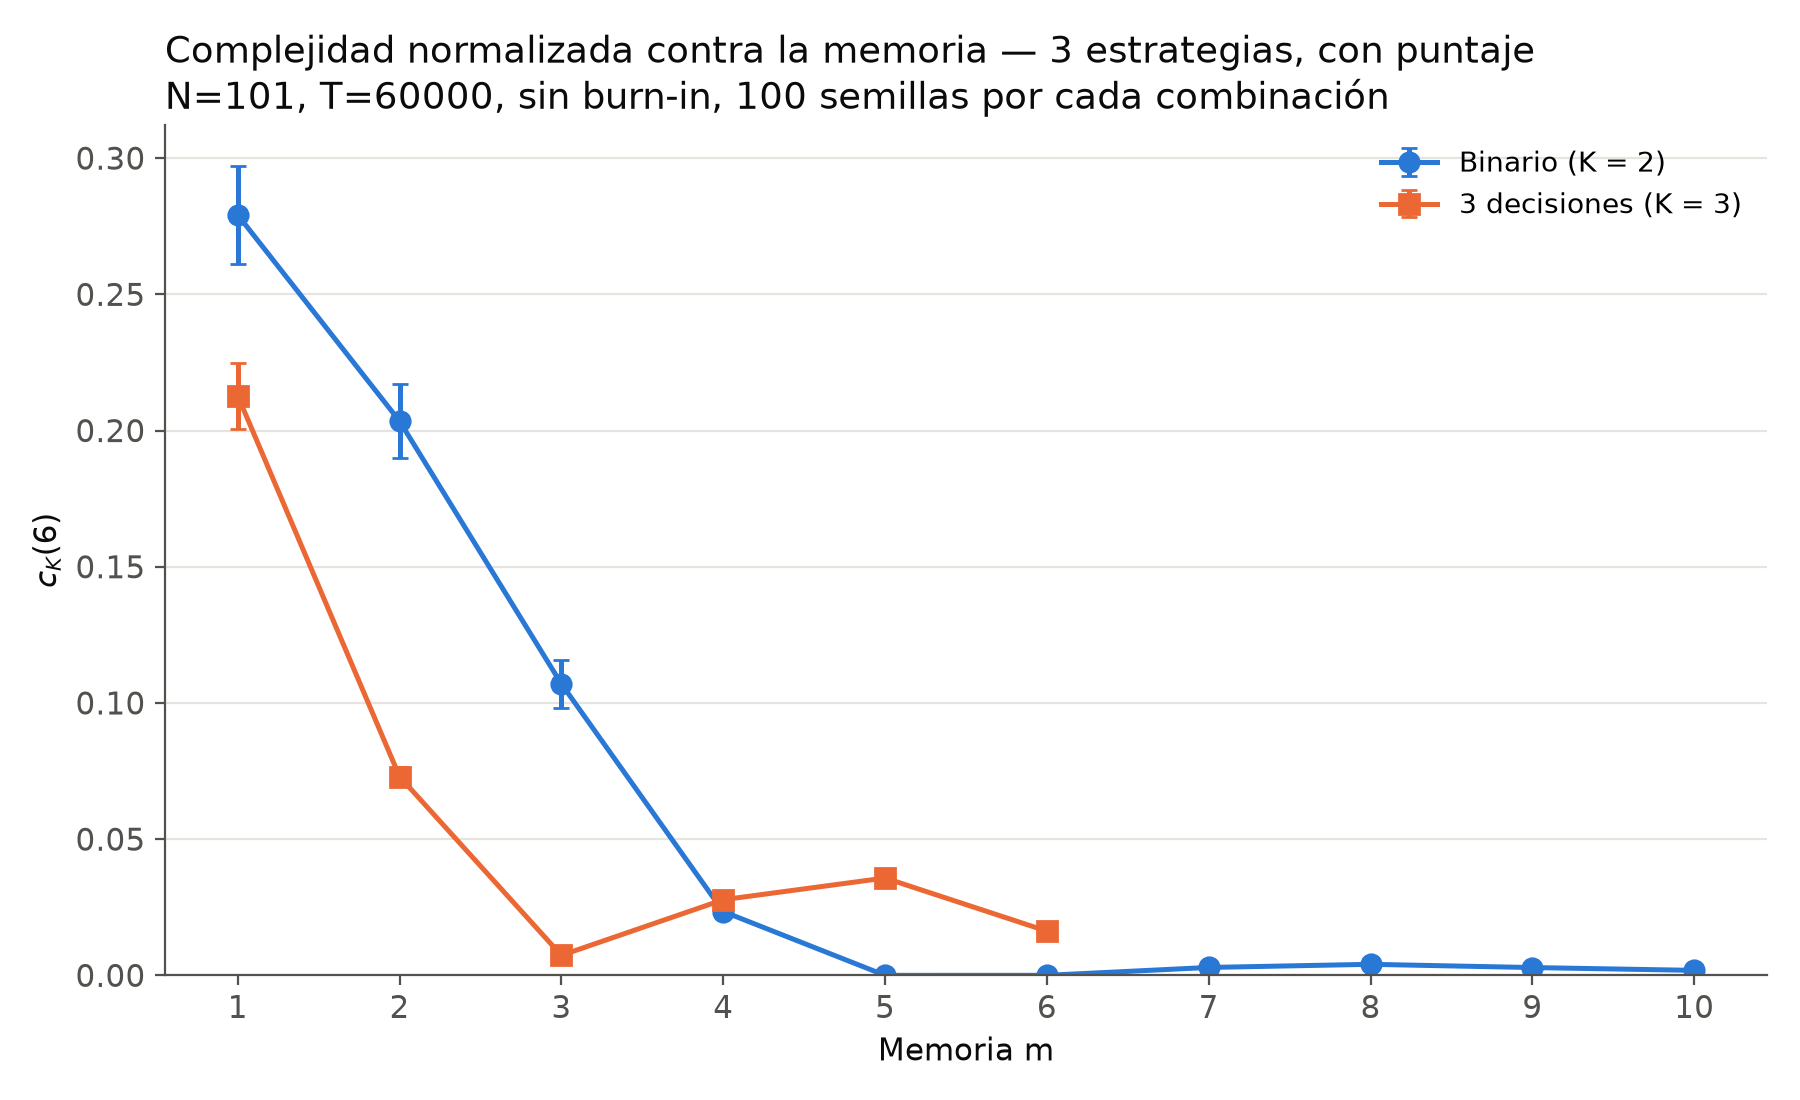
\includegraphics[width=0.8\textwidth]{figuras/Fase8_comparacion_c6_contra_m_con_puntaje_N101_s3_T60000.png}
\caption{Comparación, $s=3$: $c_K(6)$ contra $m$, con intervalo de confianza del 95\%.}
\end{figure}
\begin{figure}[H]
\centering
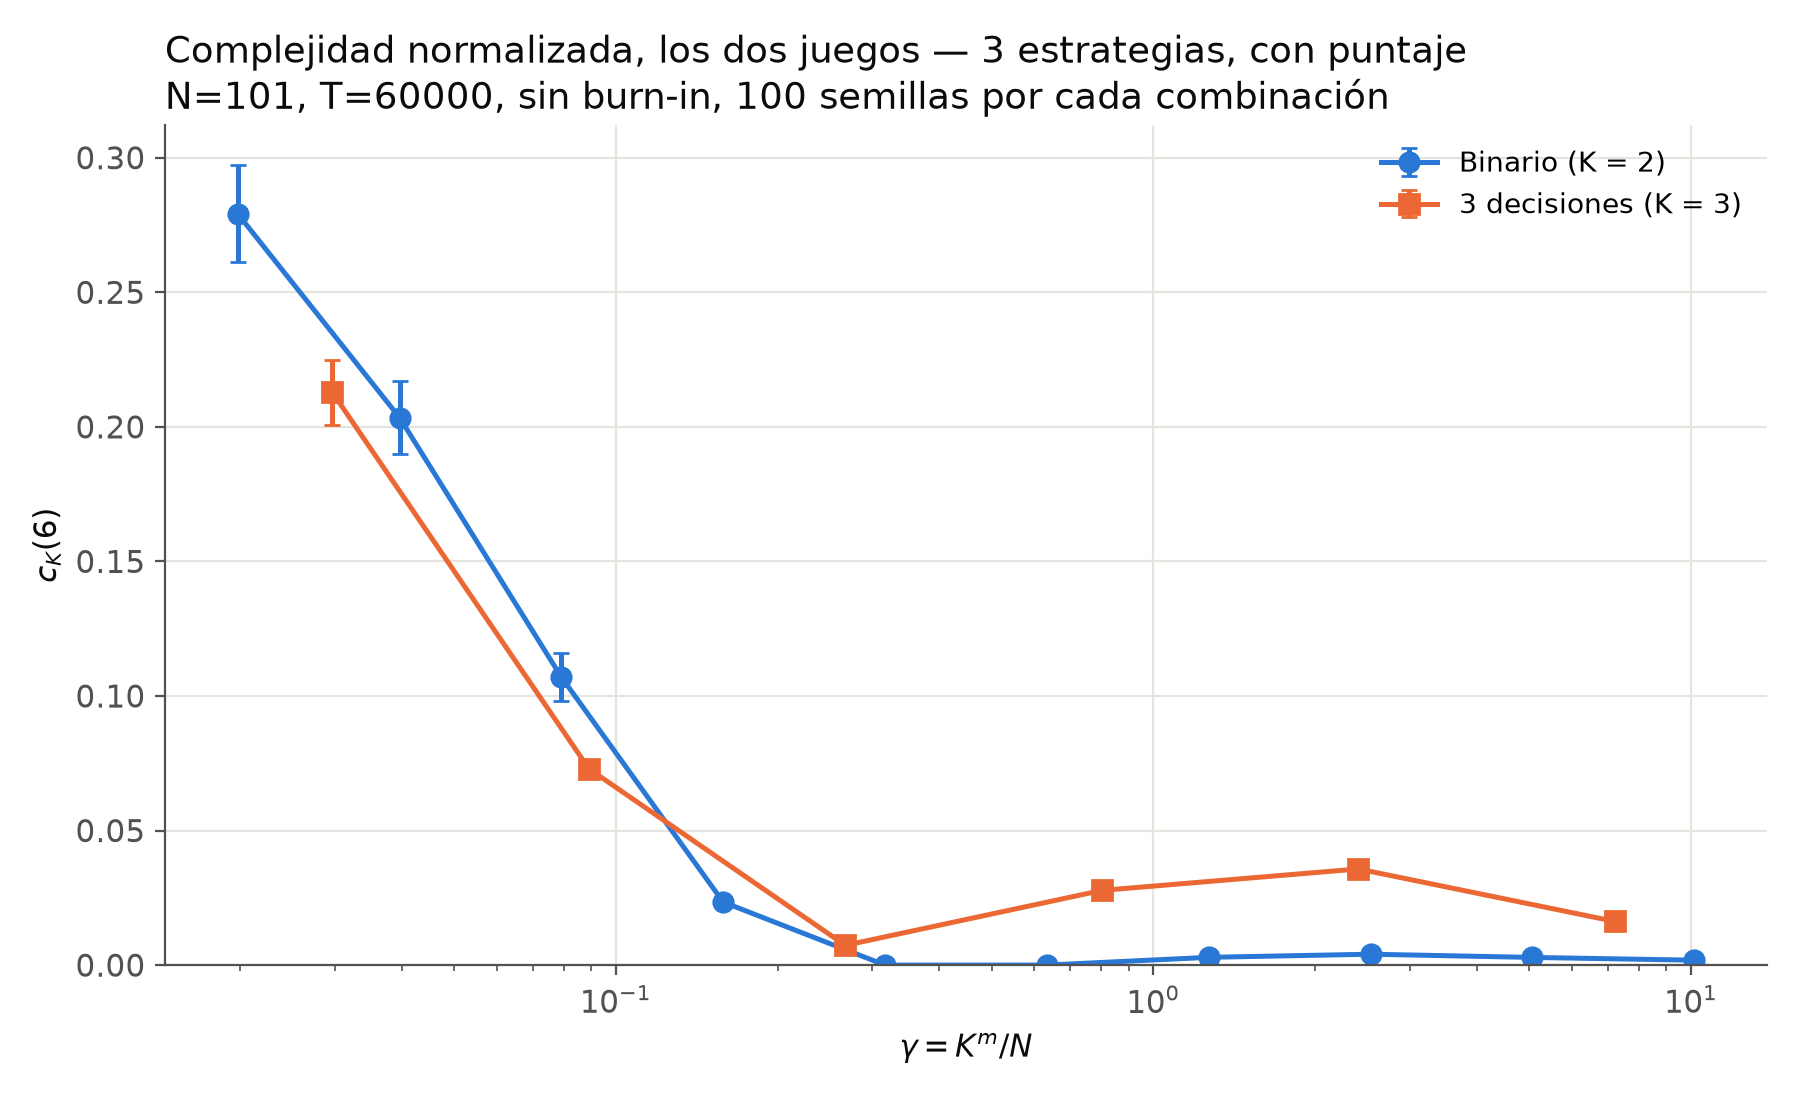
\includegraphics[width=0.8\textwidth]{figuras/Fase8_comparacion_c6_contra_gamma_con_puntaje_N101_s3_T60000.png}
\caption{Comparación, $s=3$: $c_K(6)$ contra $\gamma=K^m/N$.}
\end{figure}
\begin{figure}[H]
\centering
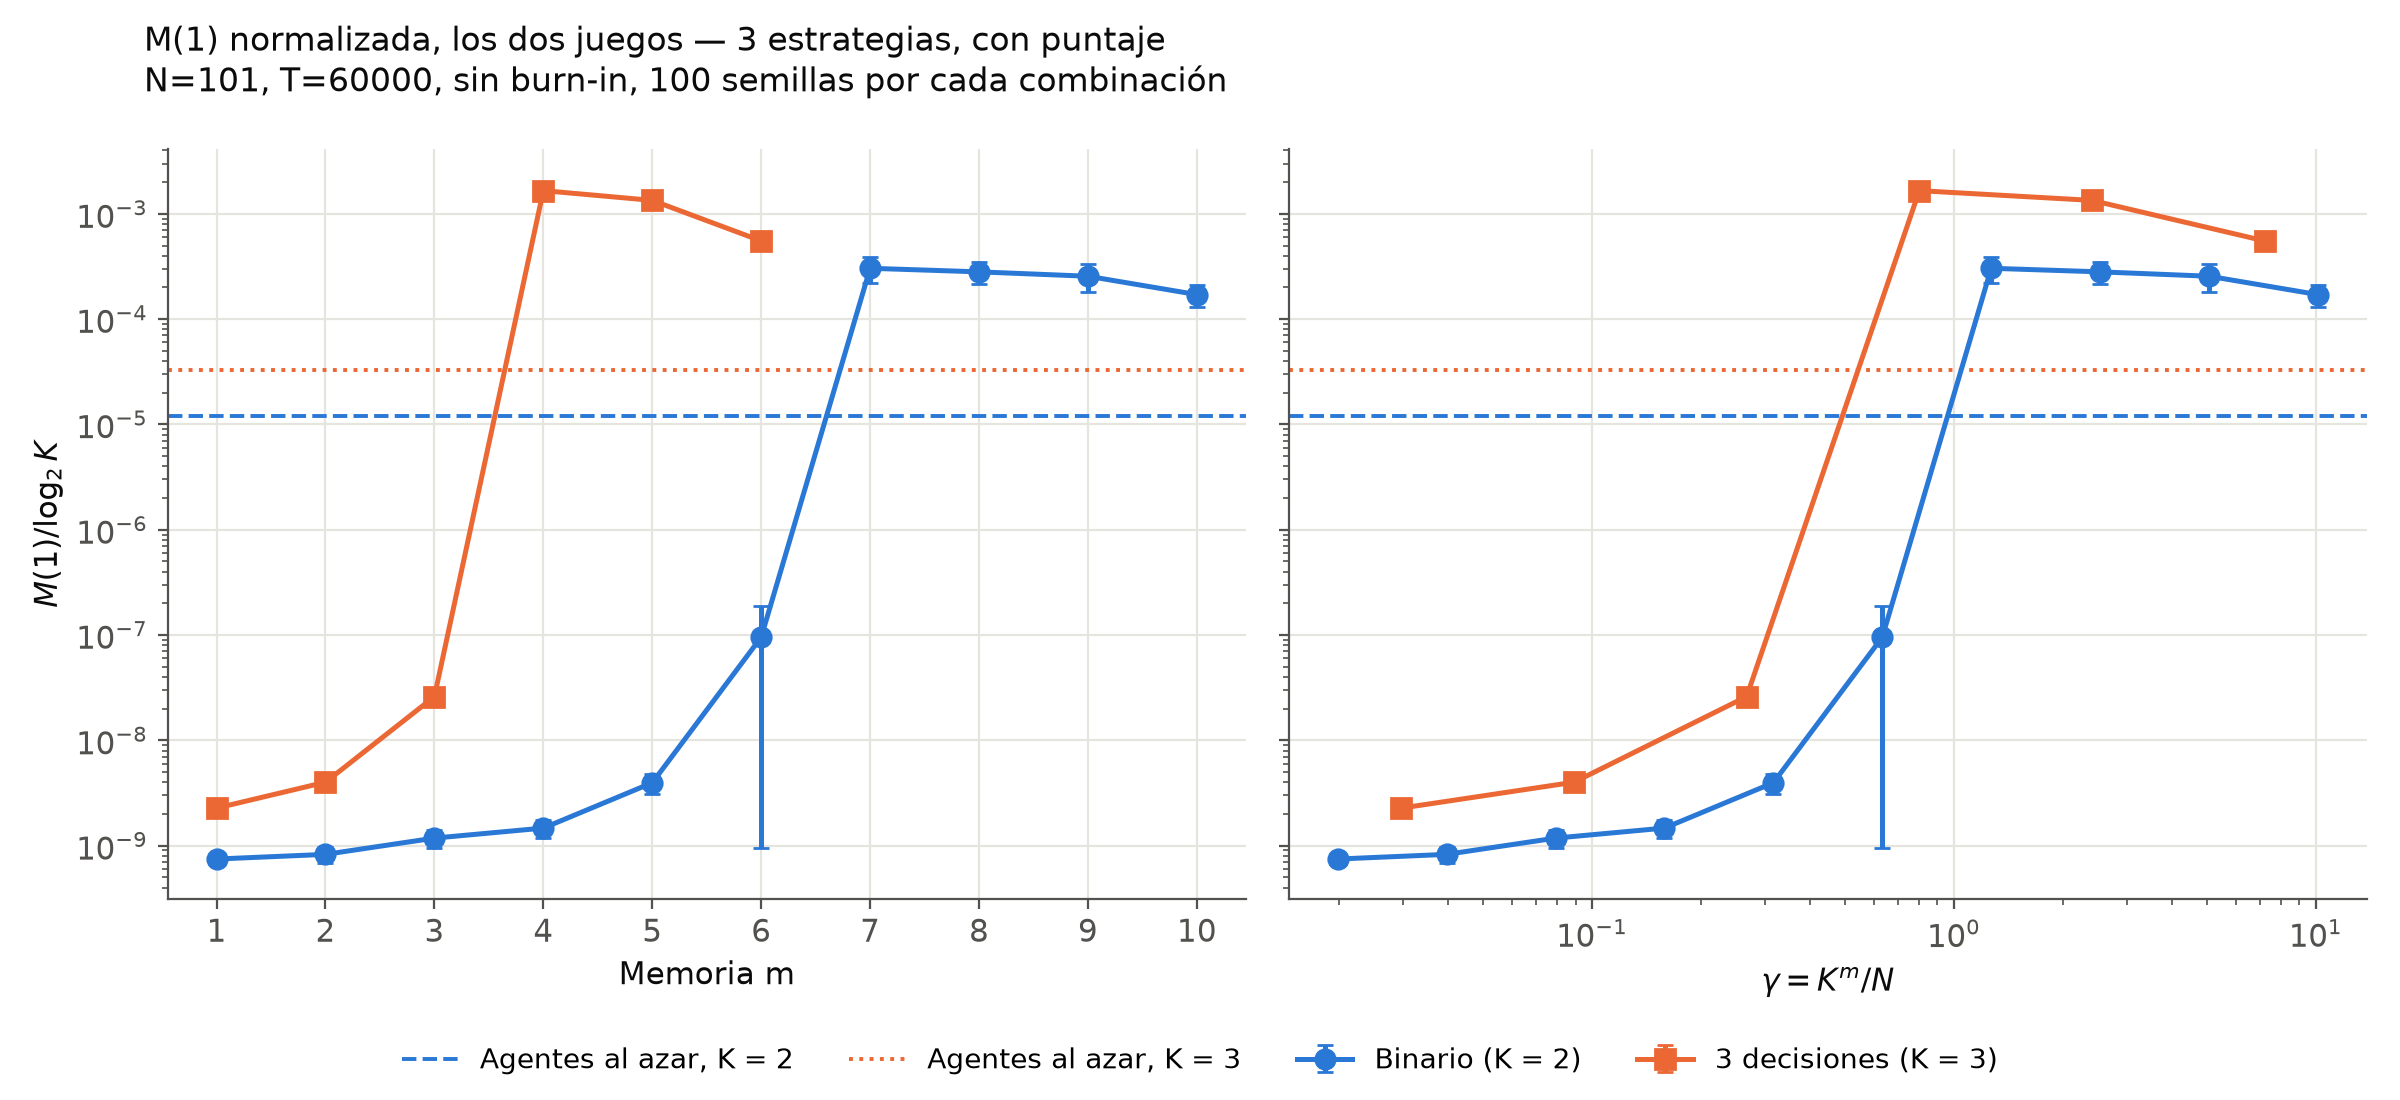
\includegraphics[width=0.92\textwidth]{figuras/Fase8_comparacion_M1_con_puntaje_N101_s3_T60000.png}
\caption{Comparación, $s=3$: $M(1)/\log_2 K$ contra $m$ y contra $\gamma$, con la referencia normalizada de cada juego.}
\end{figure}


\begin{table}[H]
\centering
\footnotesize
\setlength{\tabcolsep}{3.5pt}
\caption{Comparación de $c_K(6)$ a igual $\gamma$, con $s=2$. El valor binario se interpola linealmente en $\log\gamma$, porque los dos juegos no tienen puntos en los mismos $\gamma$; el cociente es $K=3$ entre $K=2$.}\label{tab:comp2}
\begin{tabular}{rrrrrrrr}
\toprule
$m$ (3 dec.) & $\gamma$ & $c_K(6)$, $K=3$ & IC 95\% & $c_K(6)$, $K=2$ & IC 95\% & Cociente & ¿Traslape? \\
\midrule
1 & 0.0297 & 0.25394 & [0.24131, 0.26657] & 0.29179 & [0.27377, 0.30980] & 0.87 & no \\
2 & 0.0891 & 0.05546 & [0.05345, 0.05748] & 0.10456 & [0.09728, 0.11184] & 0.53 & no \\
3 & 0.2673 & 0.06226 & [0.05710, 0.06742] & 0.00560 & [0.00455, 0.00664] & 11.1 & no \\
4 & 0.8020 & 0.09963 & [0.09703, 0.10223] & 0.01793 & [0.01630, 0.01956] & 5.56 & no \\
5 & 2.4059 & 0.07373 & [0.07258, 0.07488] & 0.01203 & [0.01130, 0.01277] & 6.13 & no \\
6 & 7.2178 & 0.03030 & [0.02981, 0.03079] & 0.00526 & [0.00489, 0.00563] & 5.76 & no \\
\bottomrule
\end{tabular}
\end{table}
\begin{table}[H]
\centering
\footnotesize
\setlength{\tabcolsep}{3.5pt}
\caption{Comparación de $c_K(6)$ a igual $\gamma$, con $s=3$. El valor binario se interpola linealmente en $\log\gamma$, porque los dos juegos no tienen puntos en los mismos $\gamma$; el cociente es $K=3$ entre $K=2$.}\label{tab:comp3}
\begin{tabular}{rrrrrrrr}
\toprule
$m$ (3 dec.) & $\gamma$ & $c_K(6)$, $K=3$ & IC 95\% & $c_K(6)$, $K=2$ & IC 95\% & Cociente & ¿Traslape? \\
\midrule
1 & 0.0297 & 0.21278 & [0.20064, 0.22491] & 0.23487 & [0.21948, 0.25025] & 0.906 & sí \\
2 & 0.0891 & 0.07296 & [0.06957, 0.07635] & 0.09280 & [0.08520, 0.10040] & 0.786 & no \\
3 & 0.2673 & 0.00734 & [0.00727, 0.00742] & 0.00574 & [0.00530, 0.00618] & 1.28 & no \\
4 & 0.8020 & 0.02776 & [0.02666, 0.02885] & 0.00099 & [0.00089, 0.00109] & 28.1 & no \\
5 & 2.4059 & 0.03573 & [0.03515, 0.03631] & 0.00396 & [0.00371, 0.00421] & 9.02 & no \\
6 & 7.2178 & 0.01623 & [0.01600, 0.01645] & 0.00233 & [0.00218, 0.00247] & 6.97 & no \\
\bottomrule
\end{tabular}
\end{table}


\subsubsection*{Lo que se ve}
\textbf{¿Baja $c_K(6)$ más rápido con $m$ en el juego de 3 decisiones?}
\begin{itemize}
\item \textbf{Con $s=2$:} al principio sí. De $m=1$ a $m=2$, $c_K(6)$ cae por un factor de 4.6 en el juego de 3 decisiones (de 0.254 a 0.055) y de 1.4 en el binario (de 0.345 a 0.254). Pero después el juego de 3 decisiones deja de bajar, sube hasta 0.100 en $m=4$ y vuelve a bajar a 0.030 en $m=6$. El binario sigue bajando hasta 0.0017 en $m=5$. Desde $m=4$ el binario queda por debajo.
\item \textbf{Con $s=3$:} también al principio. De $m=1$ a $m=3$ el juego de 3 decisiones cae por un factor de 29 (de 0.213 a 0.0073) y el binario por 2.6 (de 0.279 a 0.107). El juego de 3 decisiones llega a su mínimo en $m=3$ y luego sube hasta 0.036 en $m=5$. El binario llega al suyo, casi cero, en $m=5$.
\end{itemize}

\textbf{¿Se enciman las curvas contra $\gamma$?}
\begin{itemize}
\item \textbf{$c_K(6)$, $s=2$:} no se enciman. Las curvas se cruzan cerca de $\gamma\approx 0.1$ a $0.16$. Con $\gamma\le 0.09$, el juego de 3 decisiones está de 13 a 47\,\% por debajo del binario. Con $\gamma\ge 0.16$ está por encima, por factores de 3 a 39. Los intervalos no se traslapan en ningún punto comparado.
\item \textbf{$c_K(6)$, $s=3$:} quedan cercanas entre $\gamma\approx 0.03$ y $0.27$, con cocientes de 0.79 a 1.28 en los puntos de la tabla, y los intervalos solo se traslapan cerca de $\gamma\approx 0.03$. Desde $\gamma\approx 0.3$ se separan: el juego de 3 decisiones queda por encima, por factores de 7 en adelante.
\item \textbf{$M(1)/\log_2 K$:} los dos juegos tienen la misma forma, un valor muy bajo seguido de un salto y un descenso lento, pero el salto ocurre en distinto $\gamma$. Fuera del salto, el juego de 3 decisiones está por encima, por un factor de 2.5 a 4 con $s=2$ y de 2.7 a 5 con $s=3$ en $\gamma\gtrsim 2$. No hay traslape en ningún punto comparado.
\end{itemize}

Los dos juegos no tienen puntos en los mismos $\gamma$, así que estas comparaciones usan interpolación y son aproximadas, sobre todo cerca del salto.

\section{Resumen del cambio de régimen}
\begin{table}[H]
\centering\small
\caption{Valores de $m$ y de $\gamma$ entre los que cambia la forma de $M(d)$, con $N=101$.}
\begin{tabular}{llll}
\toprule
Juego & $s$ & Cambio entre & Rango de $\gamma$\\
\midrule
3 decisiones & 2 & $m=2$ y $m=3$ & 0.089 a 0.267\\
3 decisiones & 3 & $m=3$ y $m=4$ & 0.267 a 0.802\\
Binario & 2 & $m=4$ y $m=6$ ($m=5$ intermedio) & 0.158 a 0.634\\
Binario & 3 & $m=6$ y $m=7$ & 0.634 a 1.267\\
\bottomrule
\end{tabular}
\end{table}

\section{Conclusiones}
Estas conclusiones describen lo que muestran las simulaciones. No se evalúa aquí ninguna hipótesis de la tesis.
\begin{enumerate}
\item El juego de 3 decisiones presenta un cambio de régimen tanto al variar $N$ con $m$ fija como al variar $m$ con $N$ fija. En ambos casos pasa de una serie con $M(1)$ casi nula y máximo en $d=m+1$ a otra con $M(d)$ casi plana hasta $d\approx m$.
\item Aumentar de $s=2$ a $s=3$ desplaza el cambio hacia una memoria mayor, en los dos juegos.
\item El juego binario presenta un cambio del mismo tipo, con memorias mayores que el de 3 decisiones. En $\gamma$, los rangos del cambio de los dos juegos coinciden en parte, pero los datos solo los ubican de forma gruesa.
\item Después del cambio, el juego de 3 decisiones tiene mayor complejidad normalizada y mayor $M(1)$ normalizada que el binario. Las curvas contra $\gamma$ no se enciman, salvo por la cercanía de $c_K(6)$ con $s=3$ en $\gamma\lesssim 0.3$.
\item La validación del juego binario reproduce la forma general de $\sigma^2/N$ y su tendencia a 0.25, pero no confirma la posición del mínimo y el encimado es parcial. Conviene resolver este punto antes de apoyarse en la comparación entre juegos.
\end{enumerate}

\section{Comprobaciones realizadas}
\begin{table}[H]
\centering\small
\caption{Comprobaciones de reproducibilidad. Todas dieron resultado idéntico con \texttt{np.array\_equal}.}
\begin{tabular}{p{7.3cm}p{7.3cm}}
\toprule
Qué se comparó & Resultado\\
\midrule
Fase 6: caso $N=50$, $m=3$, $s=2$, contra \texttt{Ref Fase 2} & $M(d)$ de todas las cadenas idéntico\\
Fase 7: caso $N=25$, $m=2$, $s=3$, $T=6000$, contra la fase 6 & $M(d)$ de todas las cadenas idéntico\\
Fase 8: $K=3$, $m=2$, $s=3$, $N=101$, $T=60000$, contra el código de la fase 7 & CSV de $M(d)$ idéntico, 100 cadenas\\
Fase 7: CSV regenerados contra la corrida original & 72 de 72 arreglos idénticos\\
Fase 8, barrido: $K=2$, $N=101$, $m=5$, $s=2$, $T=6000$, contra la validación & $\sigma^2/N$ idéntico en las 100 cadenas\\
\texttt{joblib}: un núcleo contra varios (juego binario, 30 combinaciones, 4 cadenas) & Idéntico\\
Juego binario, turno por turno (3 combinaciones) & Solo símbolos 0 y 1, los conteos suman $N$, siempre gana la minoría, sin empates\\
\bottomrule
\end{tabular}
\end{table}

\section{Limitaciones y pendientes}
\begin{itemize}
\item La causa de las diferencias en la validación del juego binario no se investigó. Hay una propuesta de tres pasos: separar la primera y la segunda mitad con los conteos guardados, repetir con $T=60000$ y agregar valores de $z$ entre 0.2 y 1.
\item Las corridas no tienen burn-in.
\item $\gamma$ avanza en saltos grandes al variar $m$, así que los valores de $m$ en los que cambia la forma ubican la transición solo de forma gruesa.
\item Los dos juegos no comparten puntos de $\gamma$. Las comparaciones cuantitativas de la tabla usan interpolación.
\item La fase 7 llega hasta $m=6$ y el barrido binario hasta $m=10$, así que los rangos de $\gamma$ coinciden solo hasta $\gamma\approx 7$.
\item En las gráficas de $M(d)$ con todas las $m$, las memorias más chicas dominan la escala.
\end{itemize}

\appendix
\section{Fase 6: gráficas por grupos de $N$}\label{ap:f6}
\begin{figure}[H]
\centering
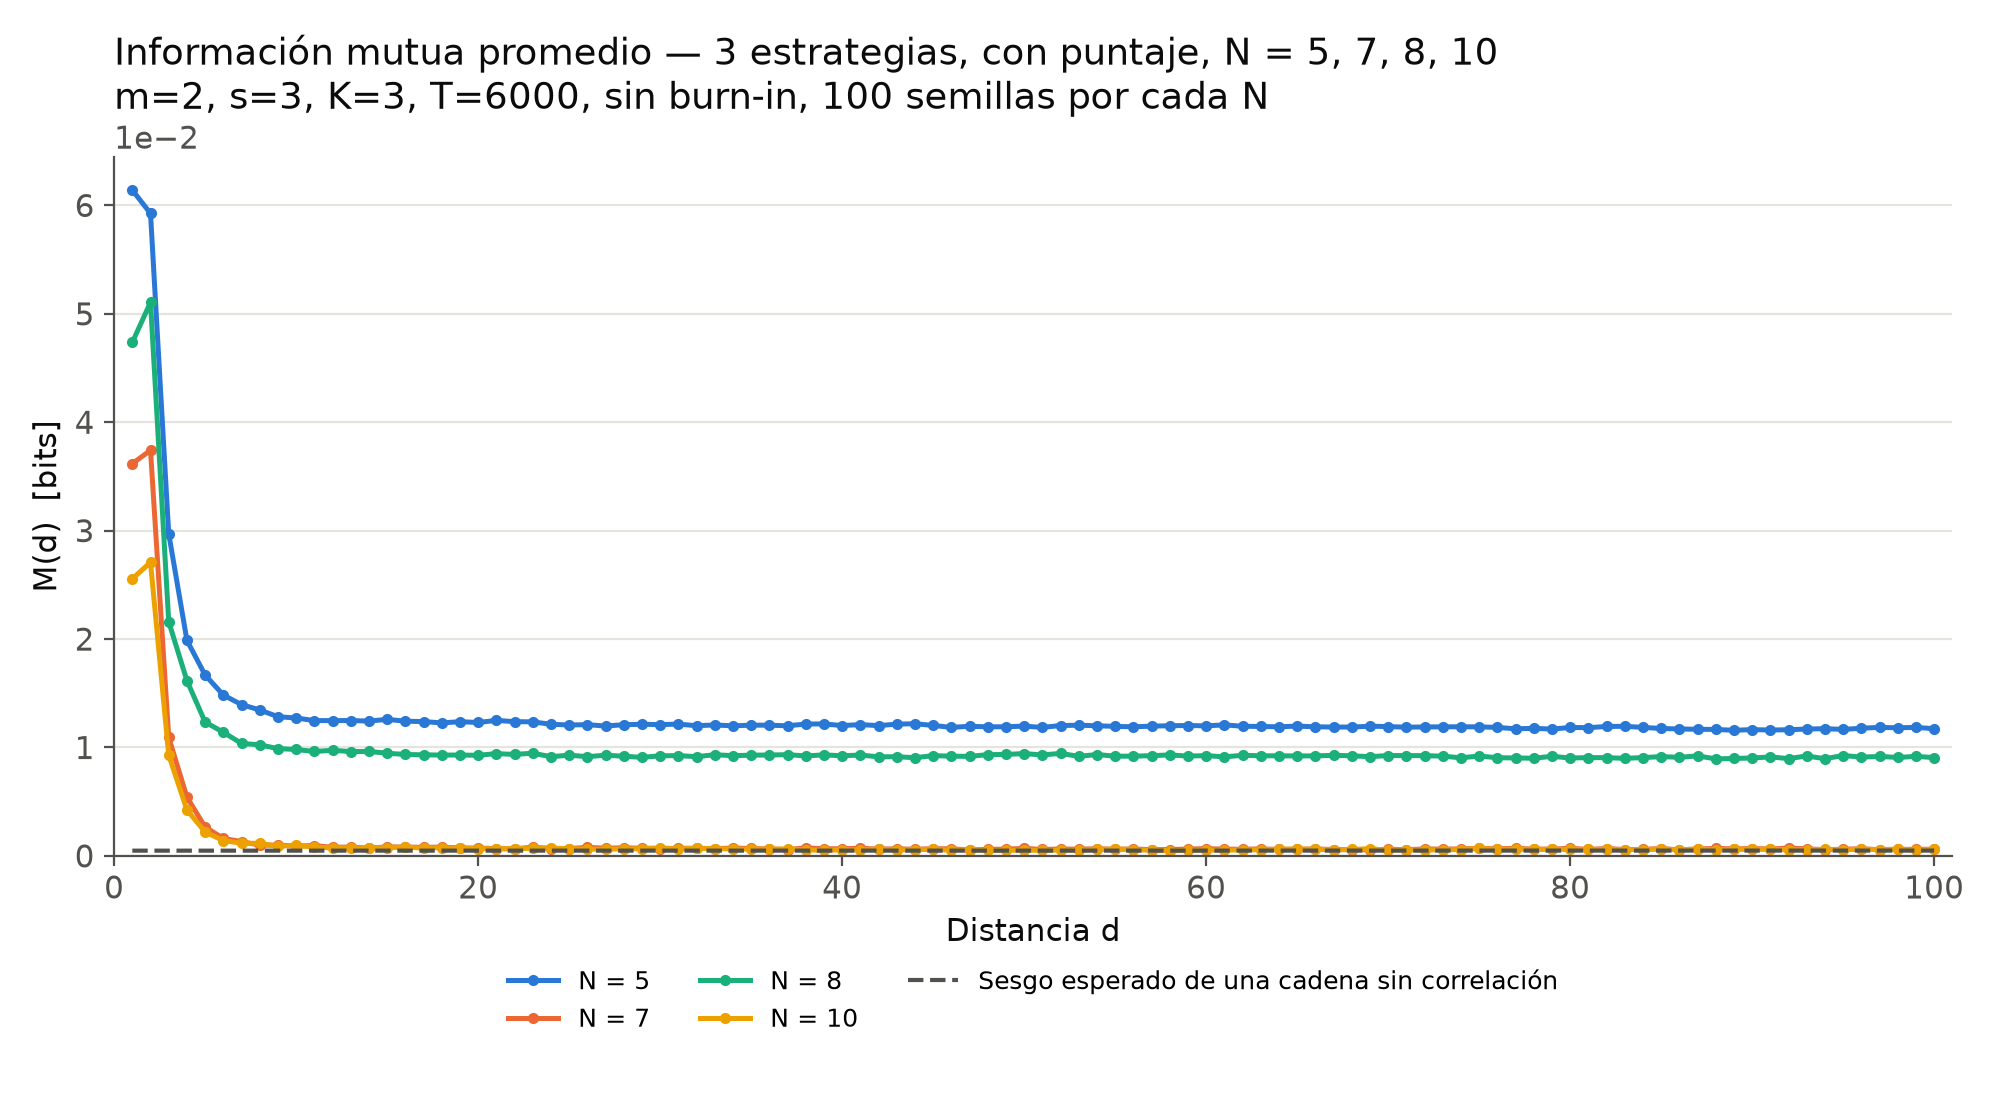
\includegraphics[width=0.49\textwidth]{figuras/Fase6_Md_con_puntaje_m2_s3_T6000_N5-7-8-10_promedio.png}\hfill
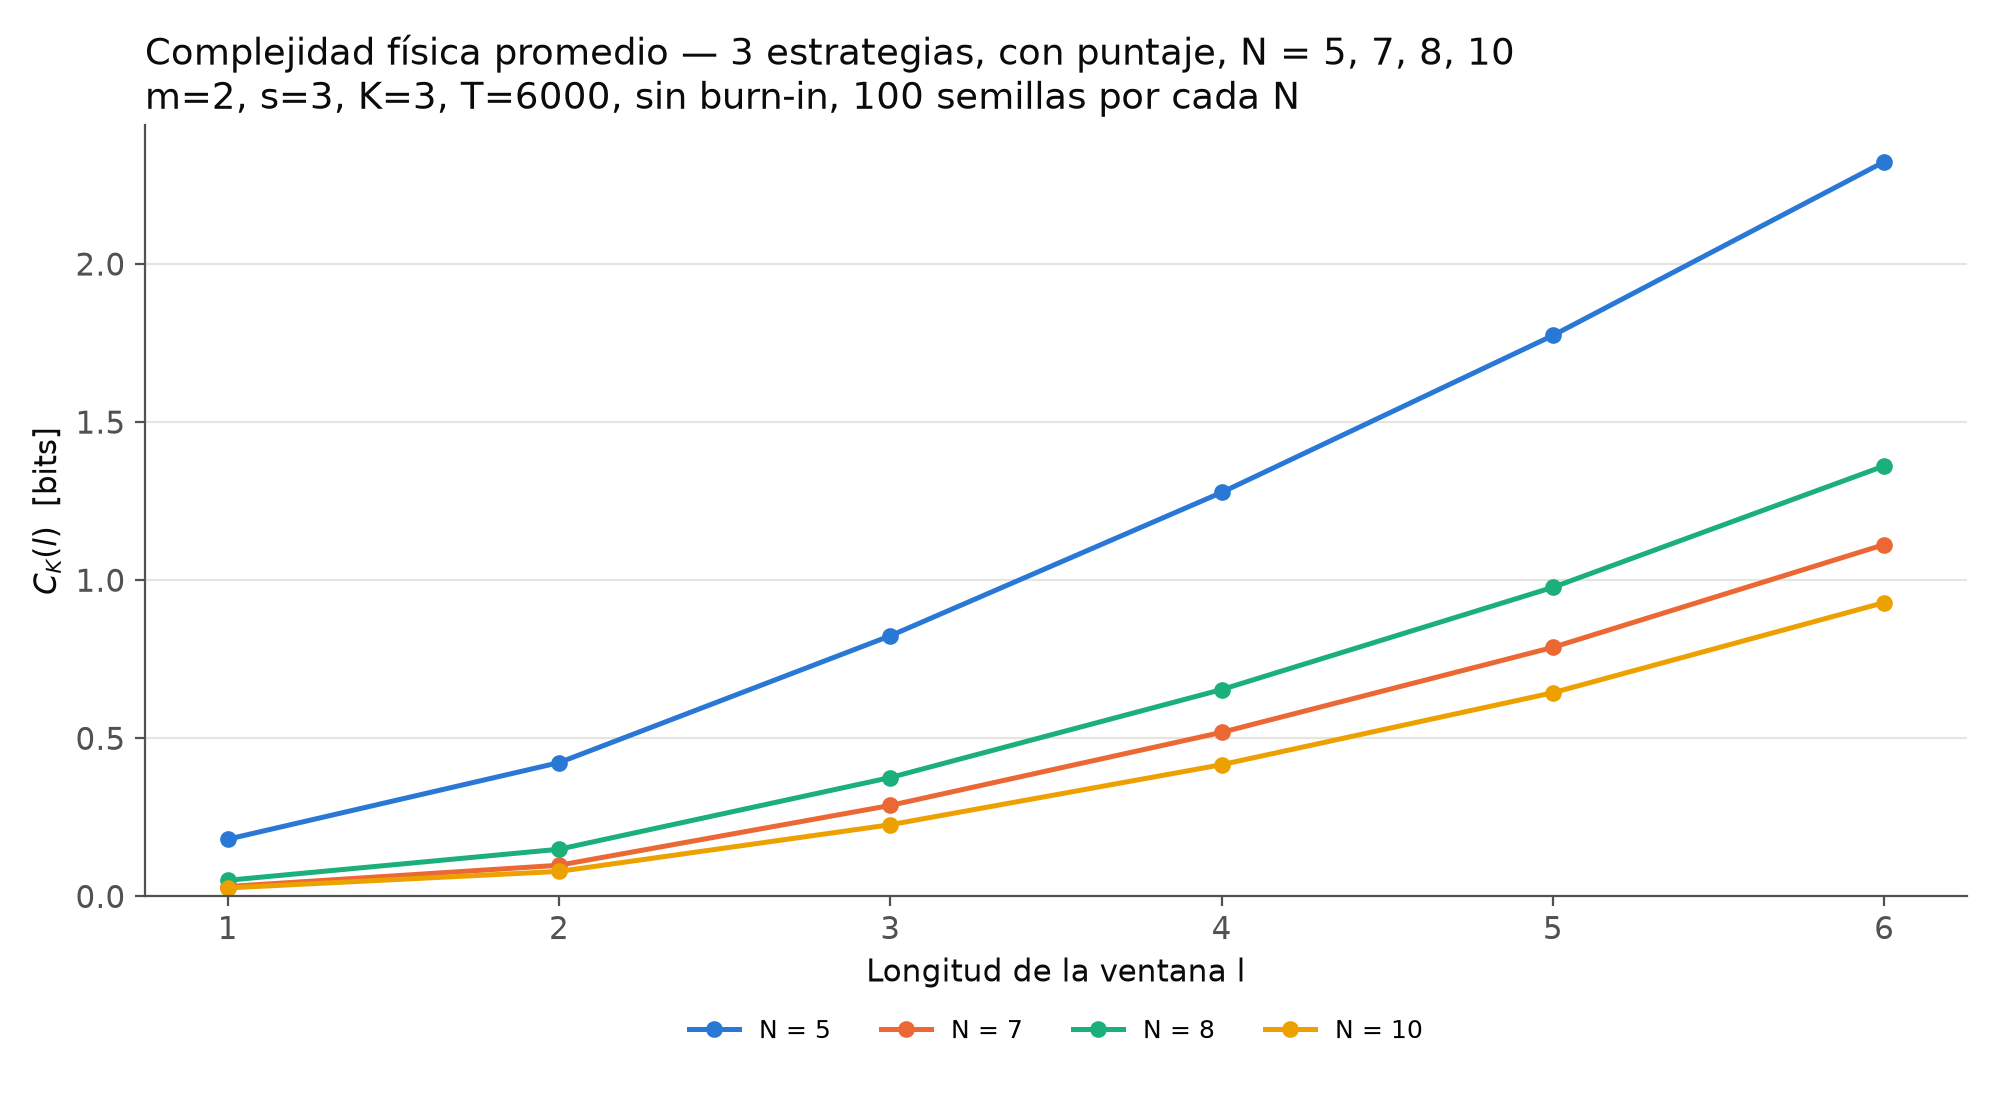
\includegraphics[width=0.49\textwidth]{figuras/Fase6_CK_con_puntaje_m2_s3_T6000_N5-7-8-10_promedio.png}
\caption{Fase 6, $N=5, 7, 8, 10$: $M(d)$ promedio (izquierda) y $C_K(l)$ promedio (derecha).}
\end{figure}
\begin{figure}[H]
\centering
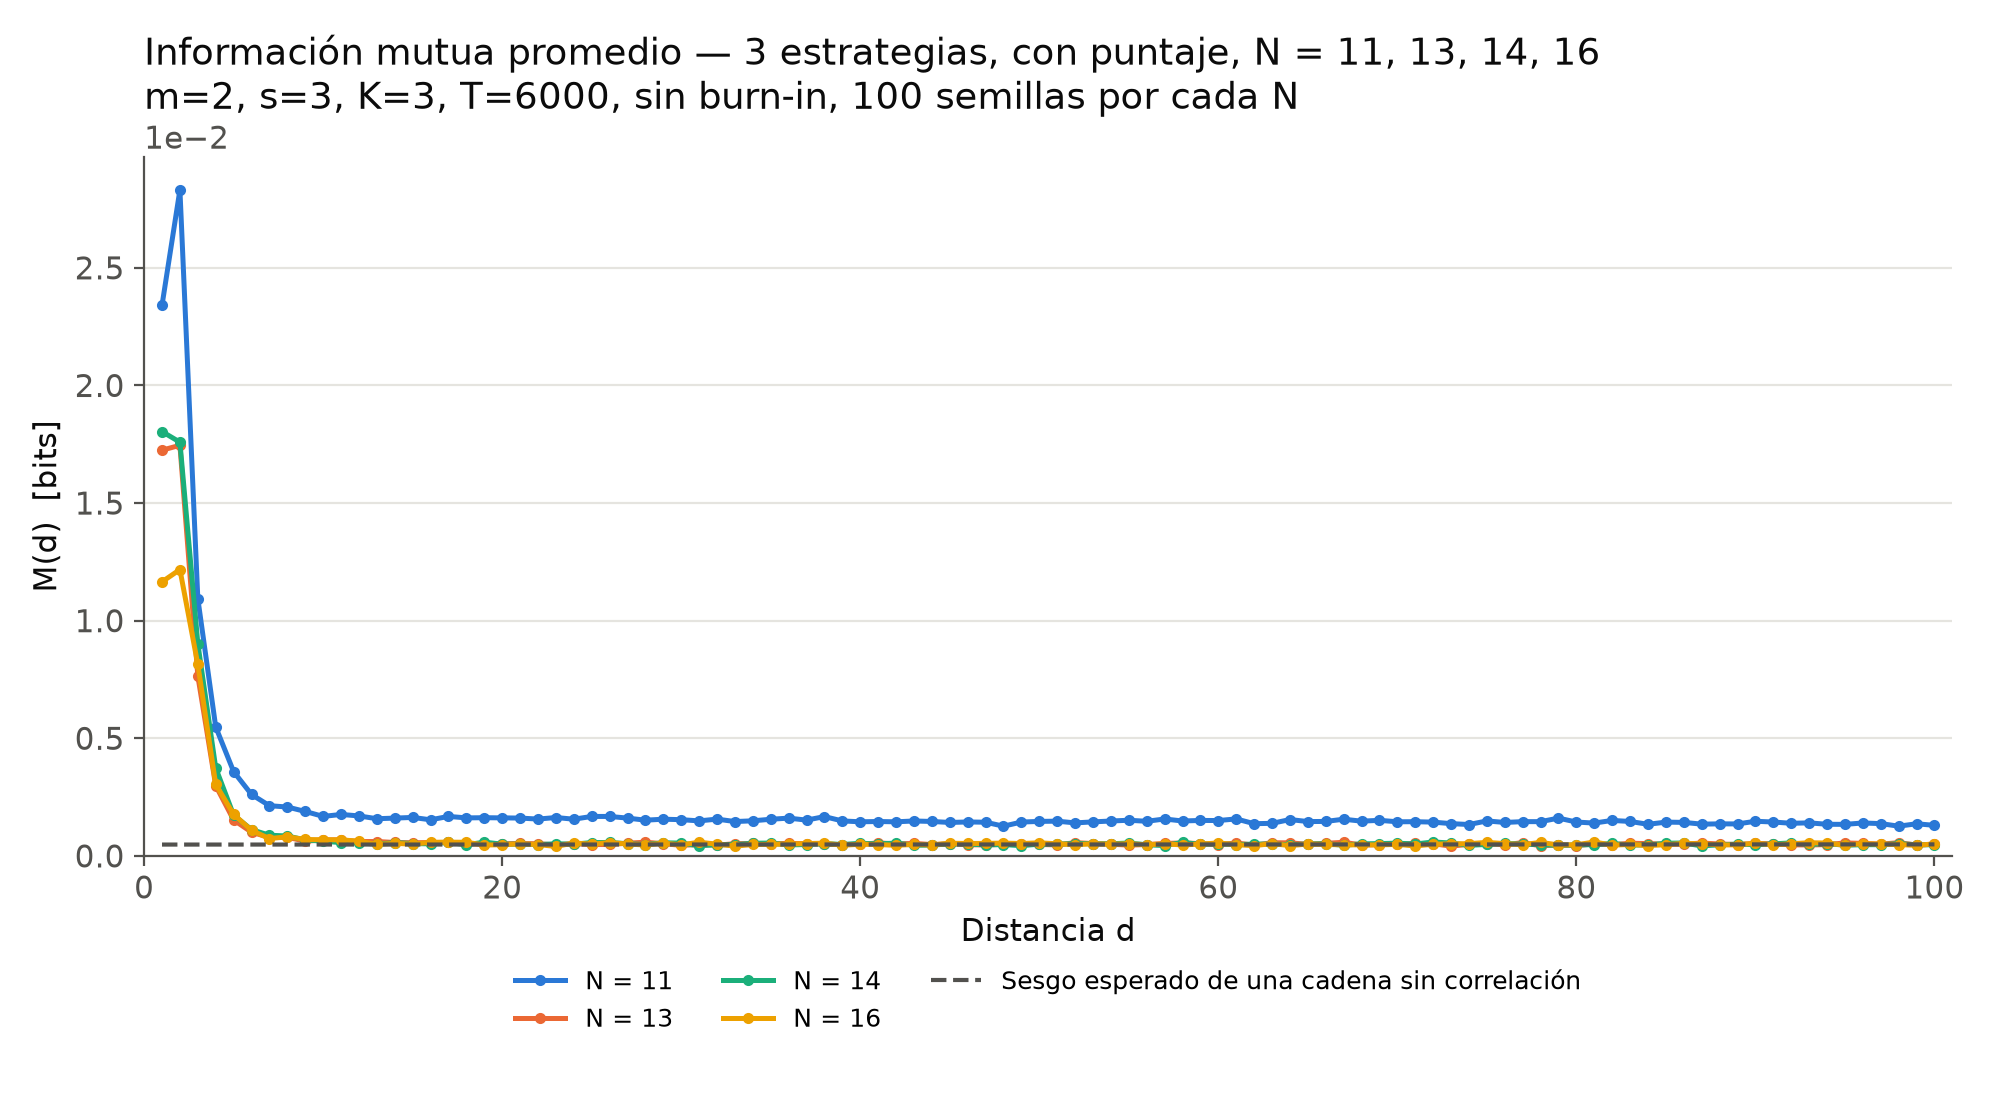
\includegraphics[width=0.49\textwidth]{figuras/Fase6_Md_con_puntaje_m2_s3_T6000_N11-13-14-16_promedio.png}\hfill
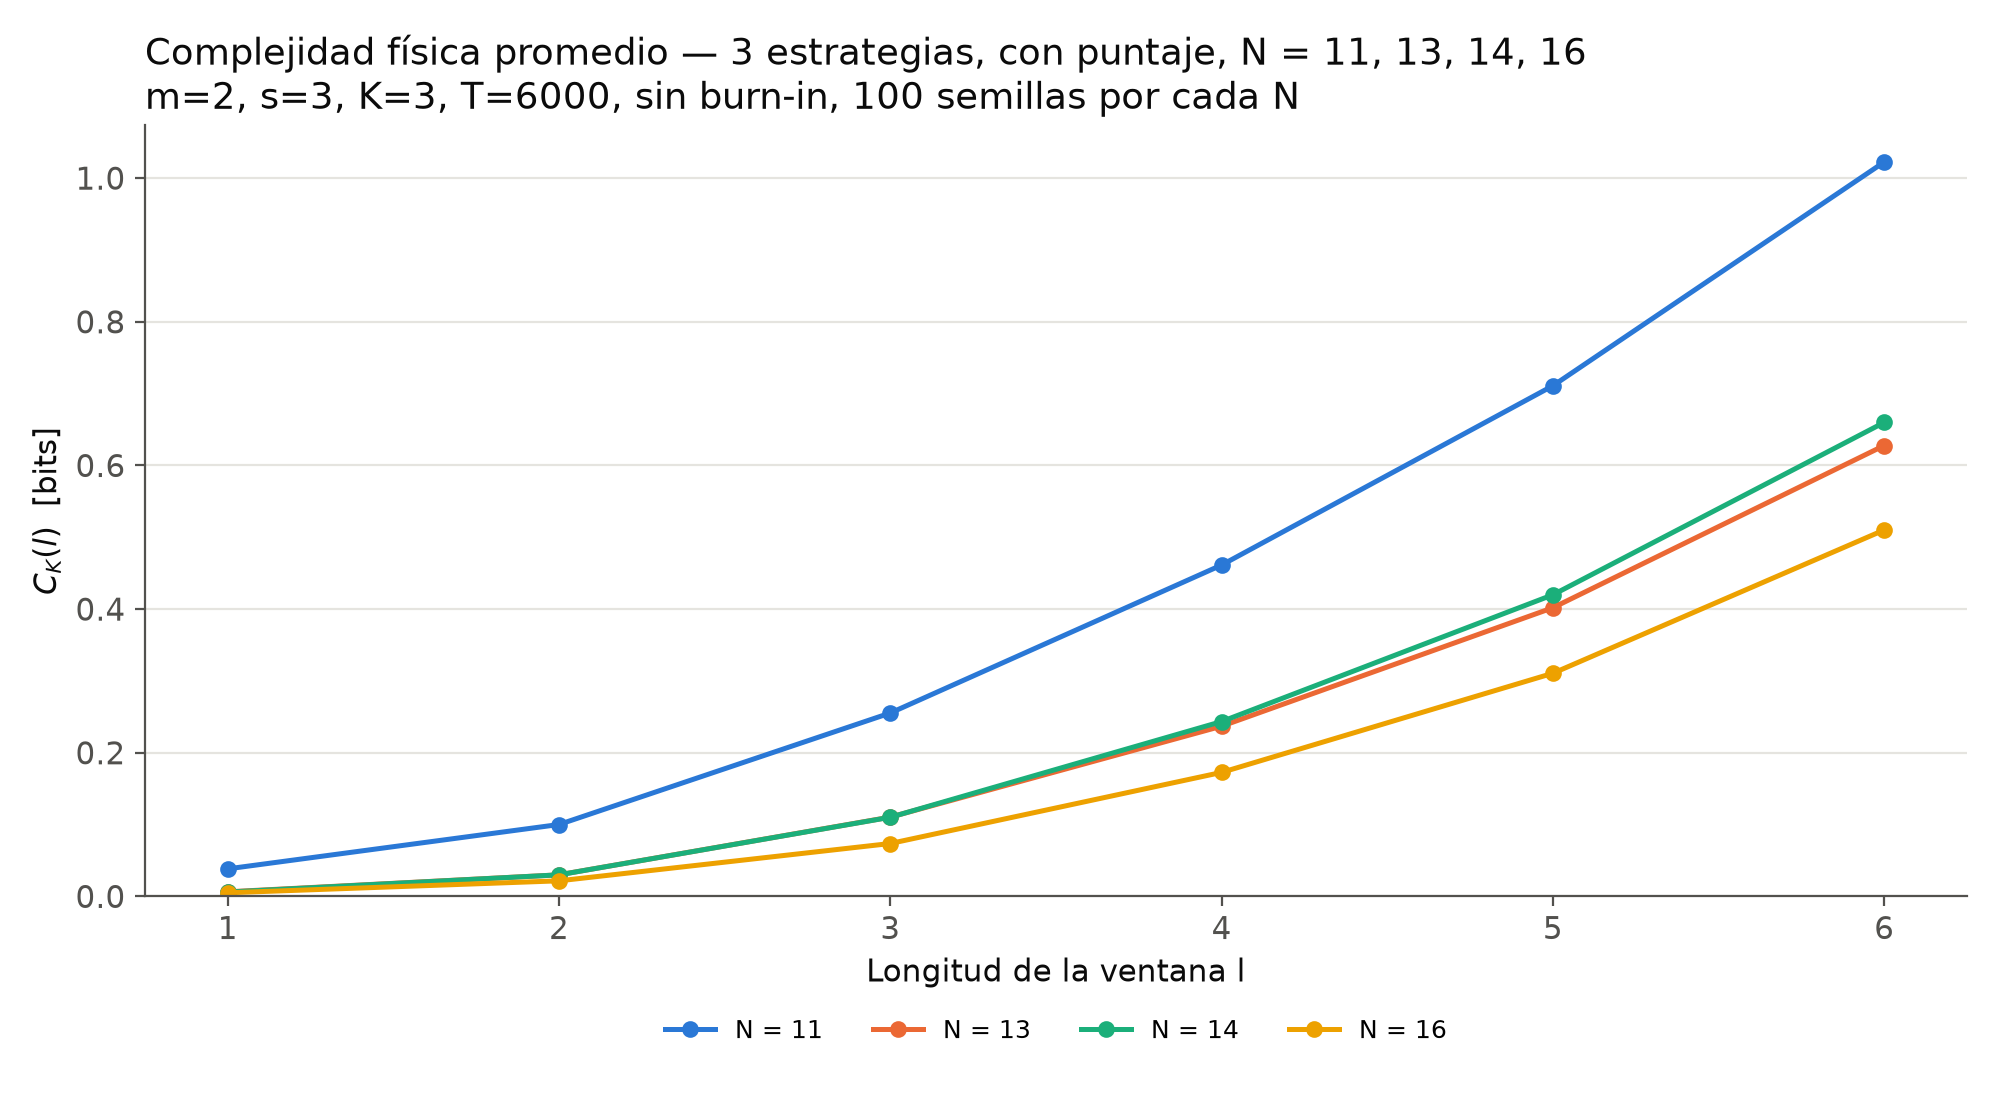
\includegraphics[width=0.49\textwidth]{figuras/Fase6_CK_con_puntaje_m2_s3_T6000_N11-13-14-16_promedio.png}
\caption{Fase 6, $N=11, 13, 14, 16$: $M(d)$ promedio (izquierda) y $C_K(l)$ promedio (derecha).}
\end{figure}
\begin{figure}[H]
\centering
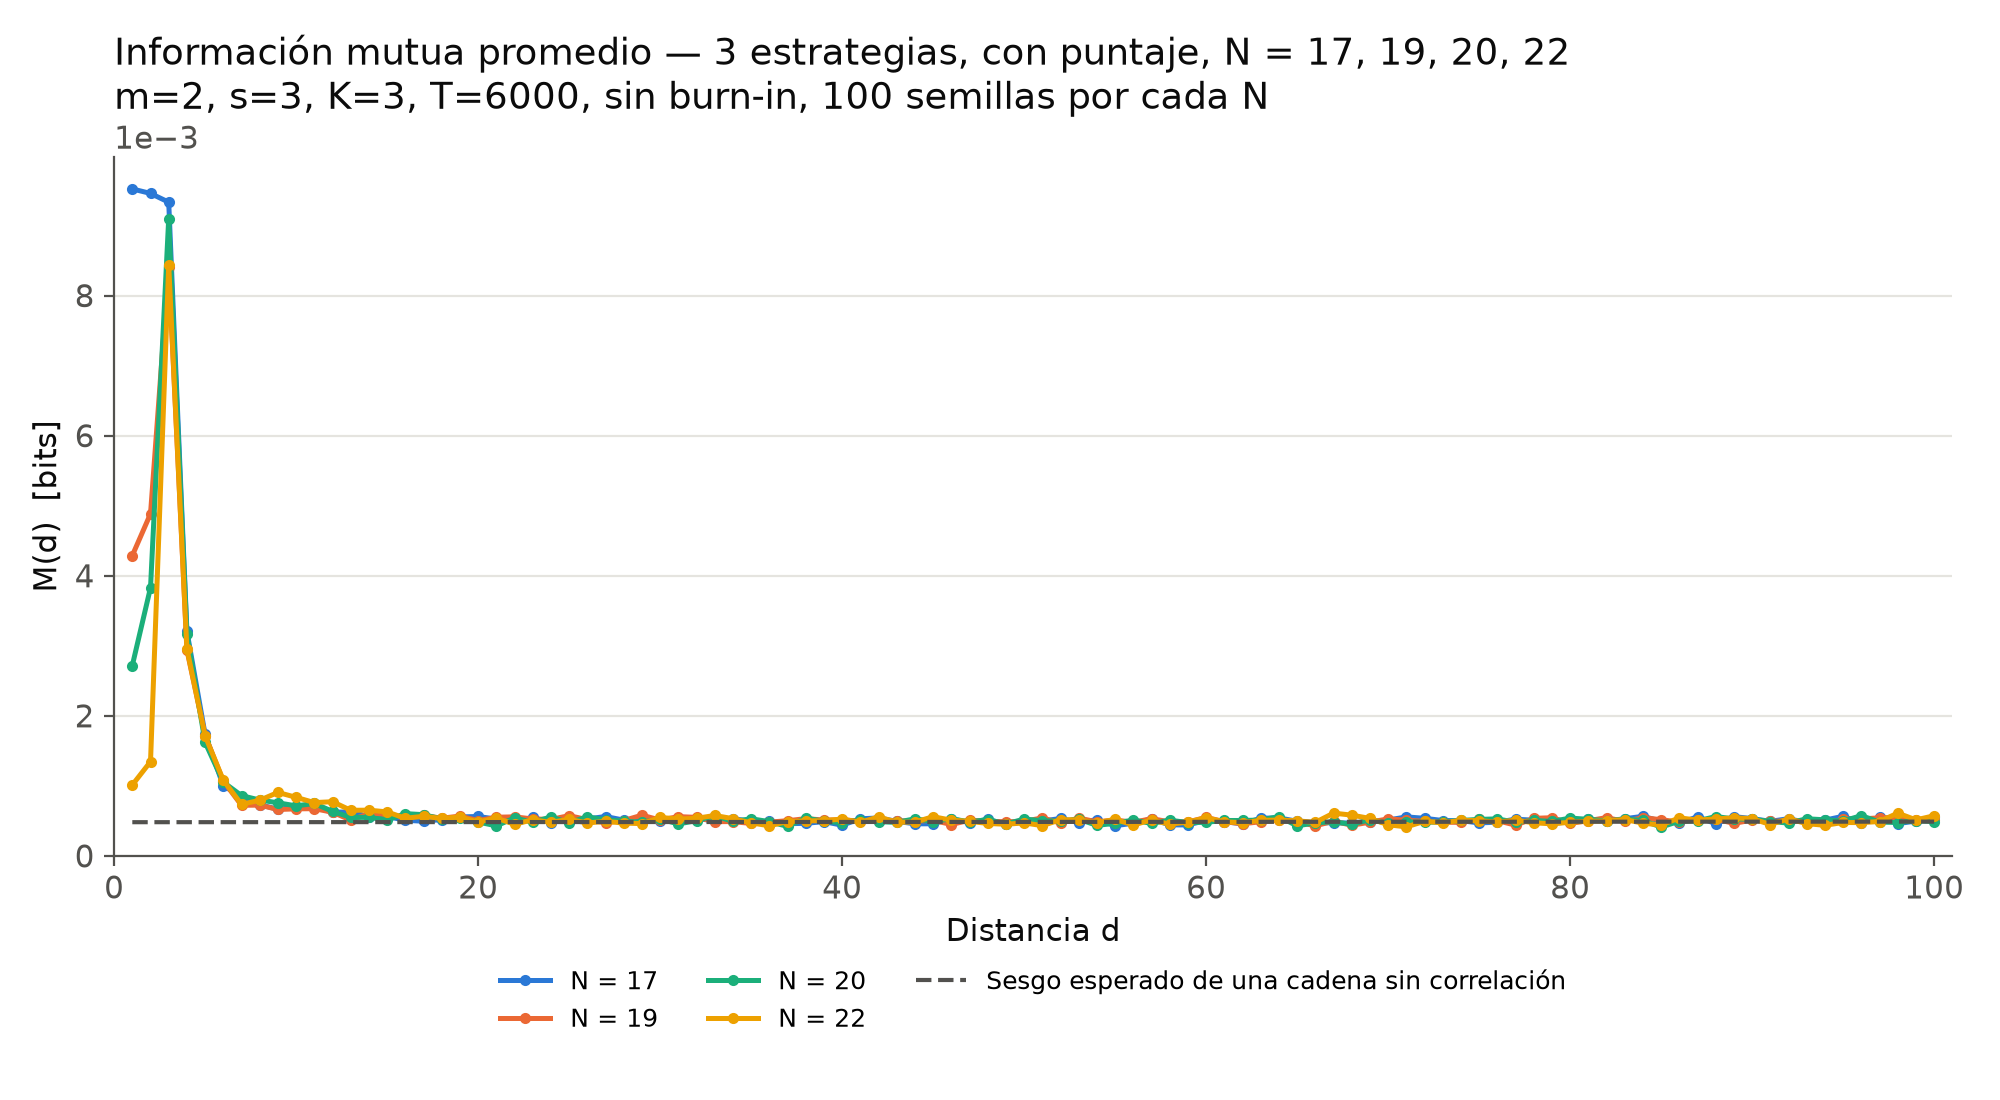
\includegraphics[width=0.49\textwidth]{figuras/Fase6_Md_con_puntaje_m2_s3_T6000_N17-19-20-22_promedio.png}\hfill
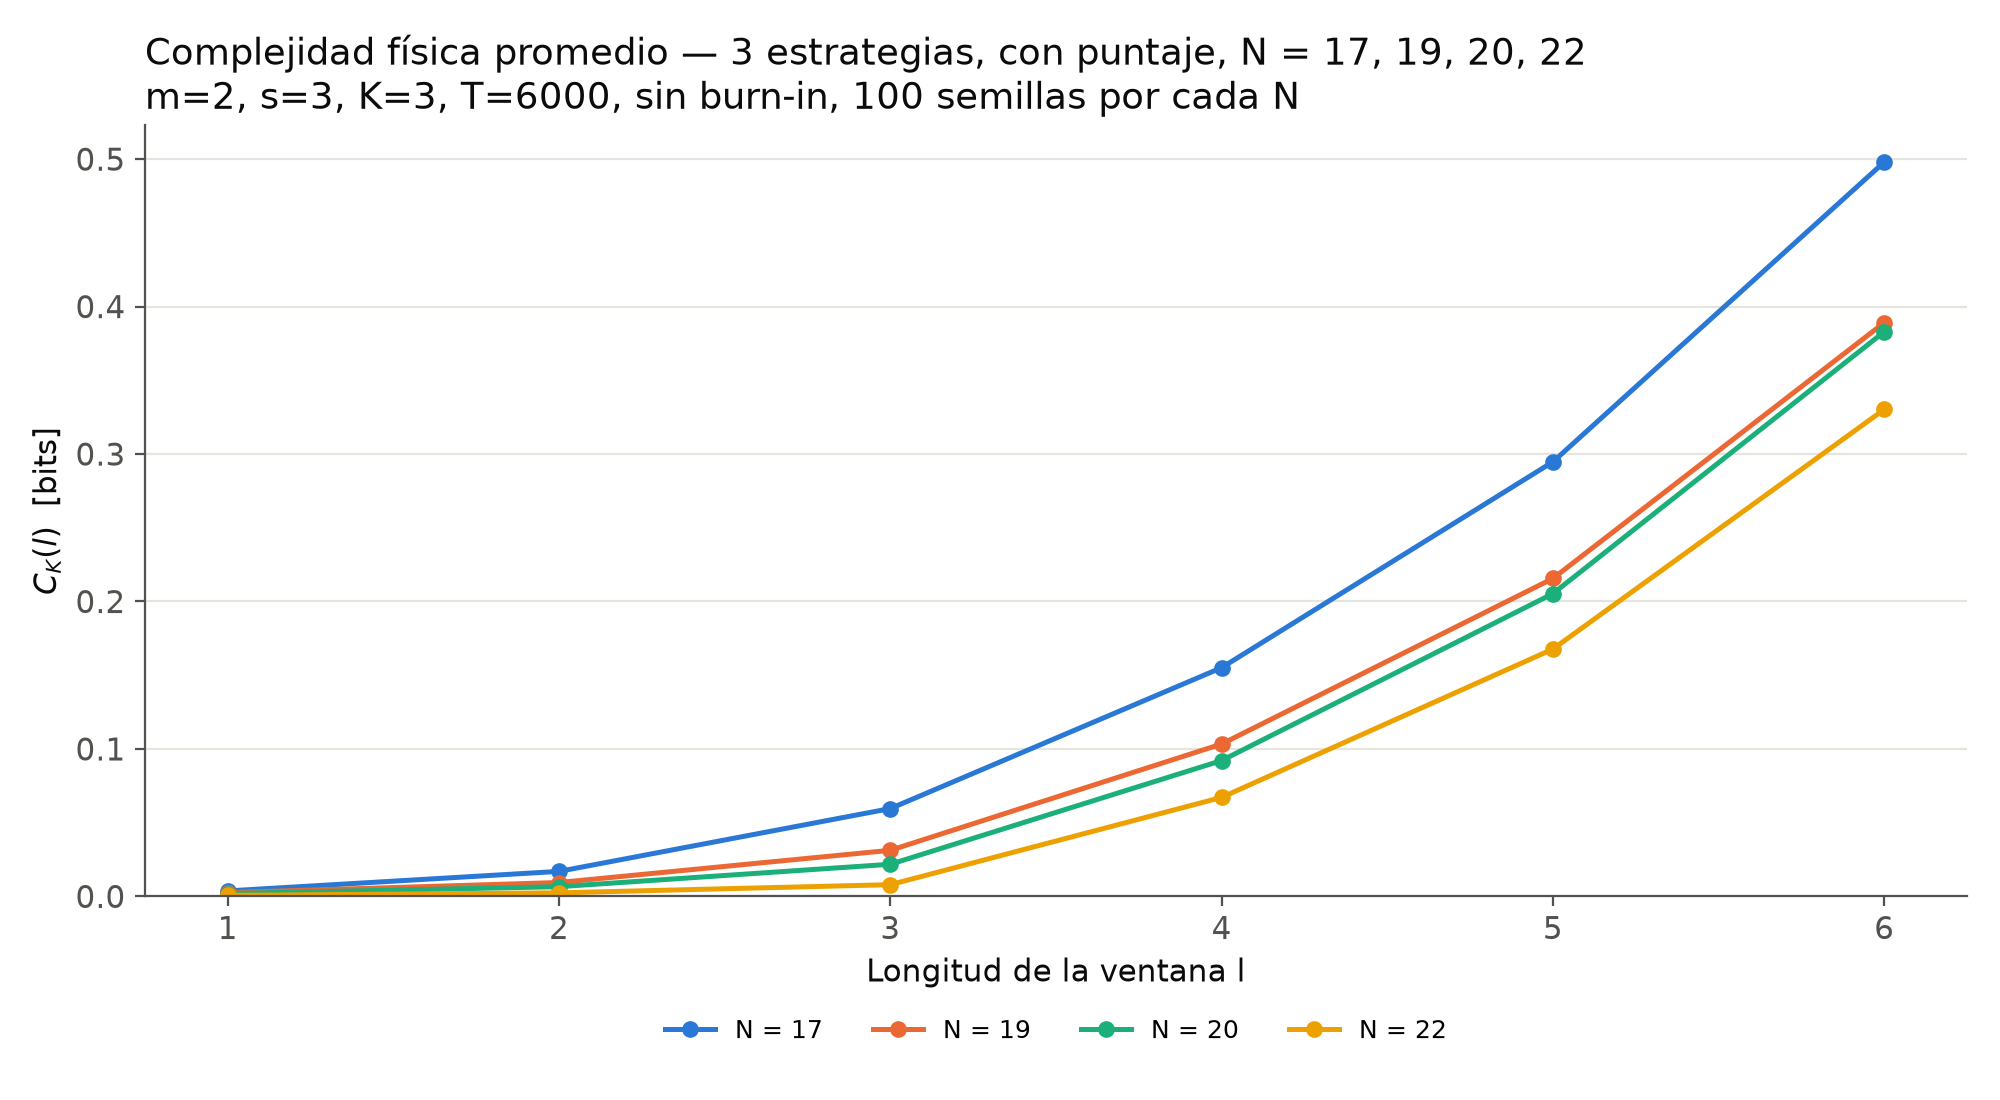
\includegraphics[width=0.49\textwidth]{figuras/Fase6_CK_con_puntaje_m2_s3_T6000_N17-19-20-22_promedio.png}
\caption{Fase 6, $N=17, 19, 20, 22$: $M(d)$ promedio (izquierda) y $C_K(l)$ promedio (derecha).}
\end{figure}
\begin{figure}[H]
\centering
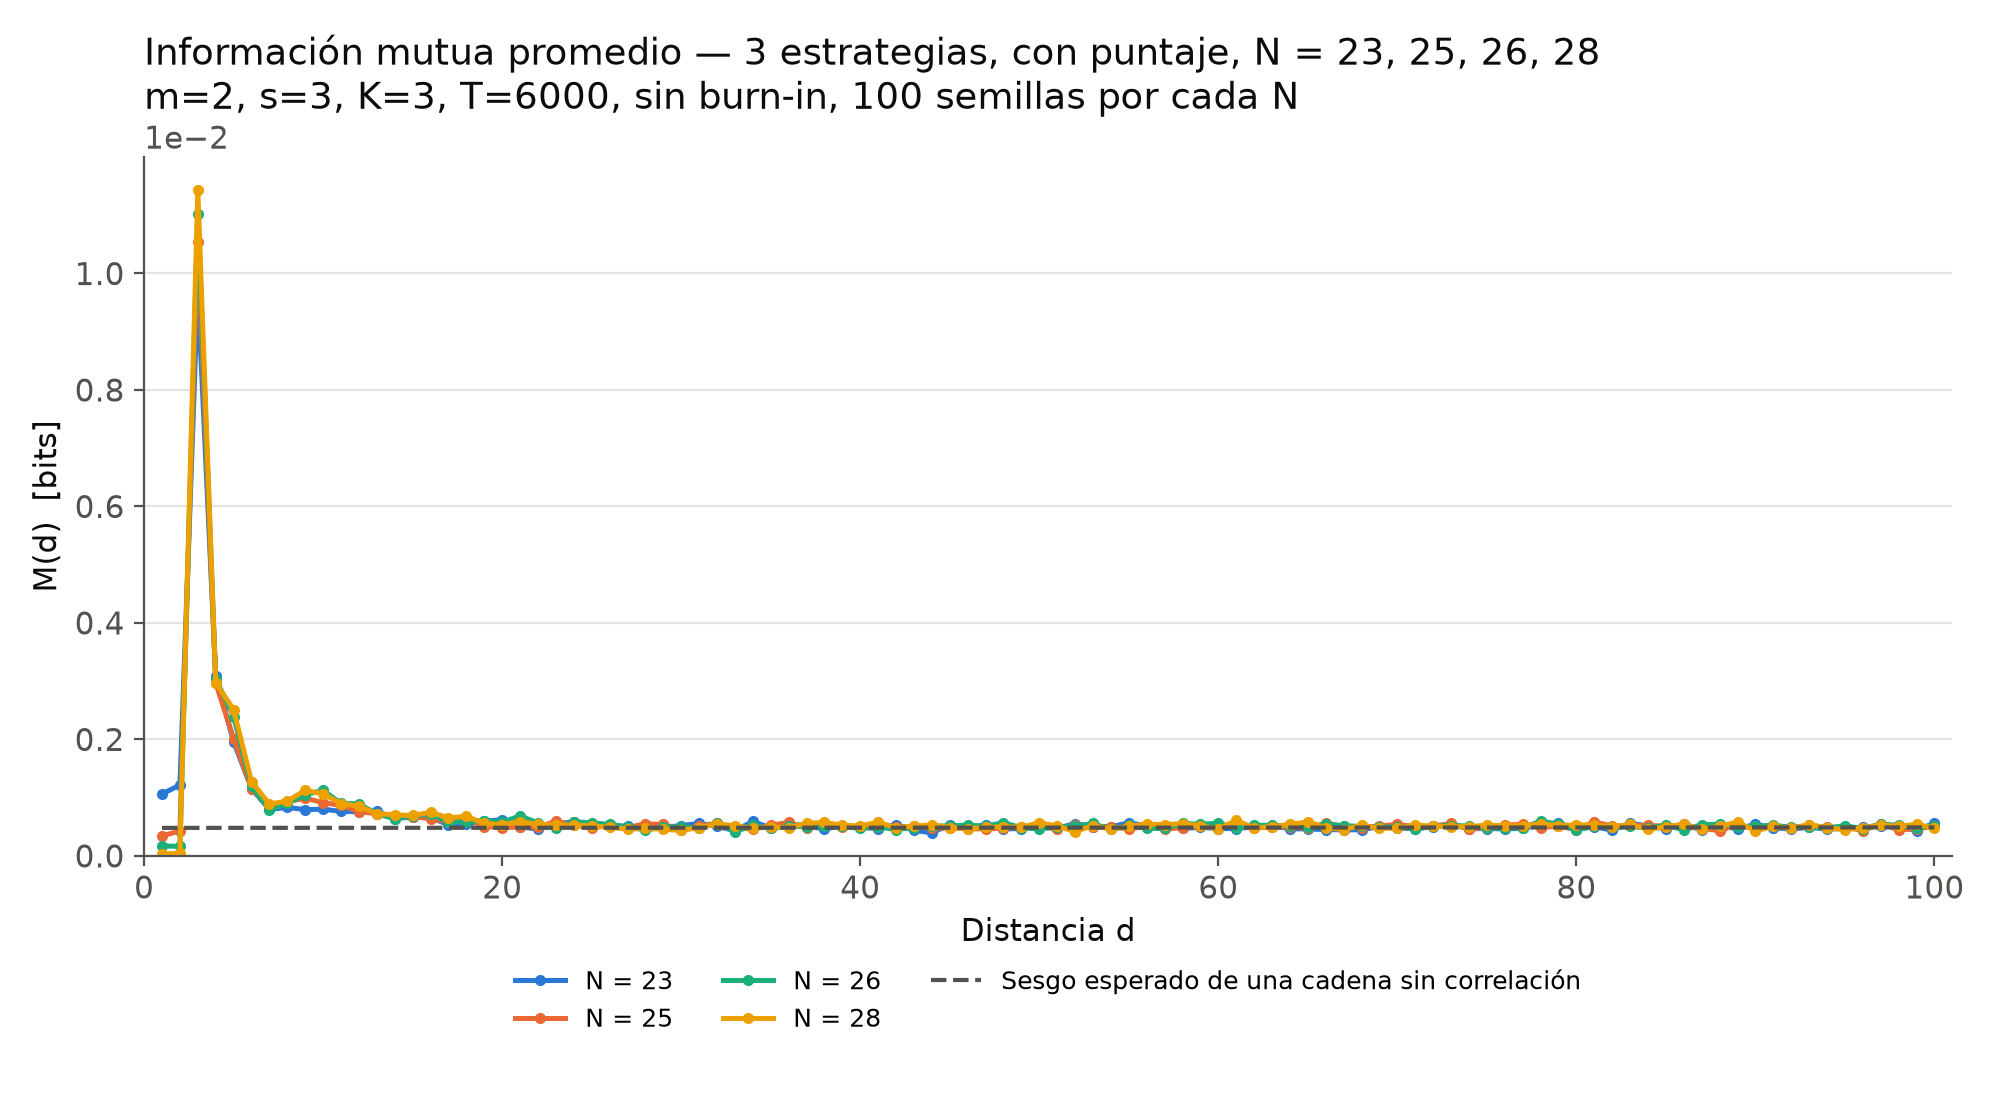
\includegraphics[width=0.49\textwidth]{figuras/Fase6_Md_con_puntaje_m2_s3_T6000_N23-25-26-28_promedio.png}\hfill
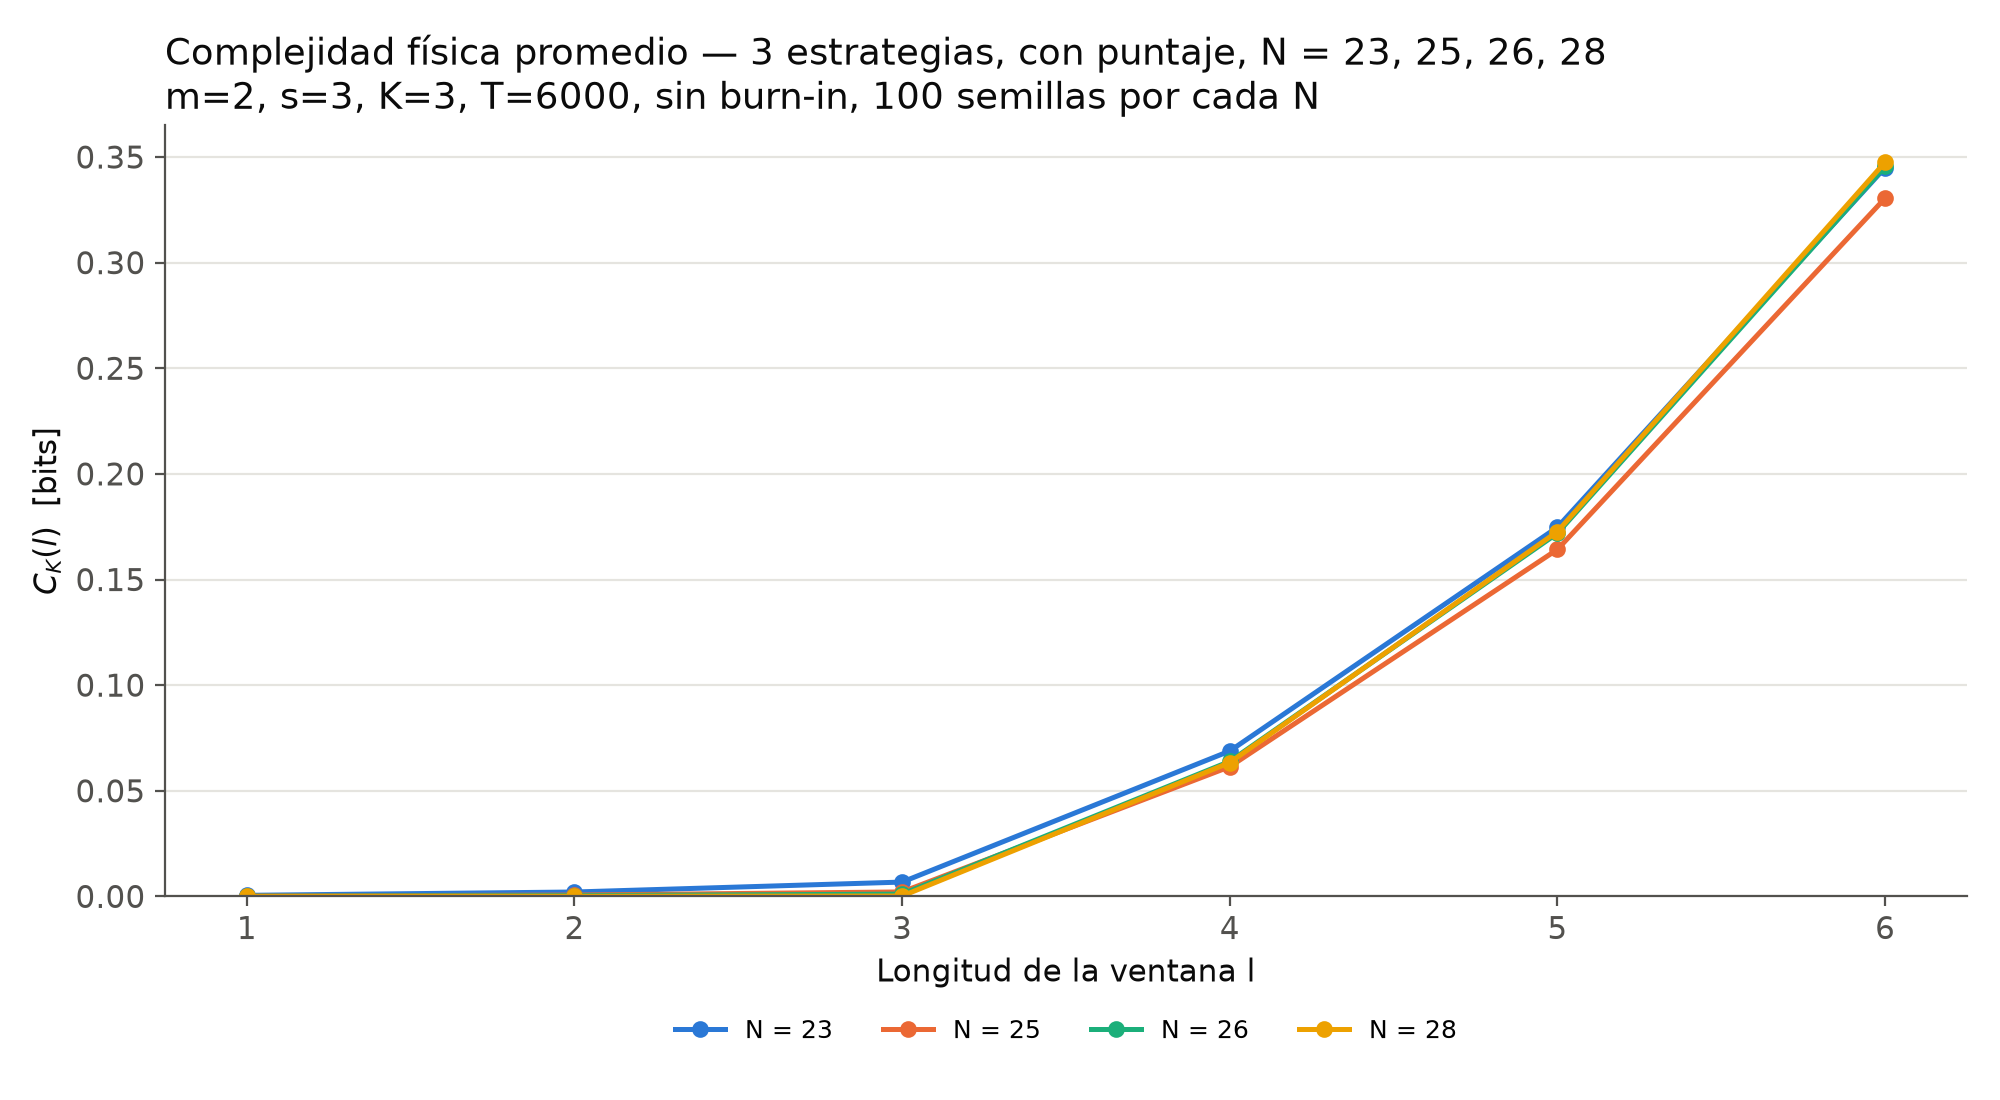
\includegraphics[width=0.49\textwidth]{figuras/Fase6_CK_con_puntaje_m2_s3_T6000_N23-25-26-28_promedio.png}
\caption{Fase 6, $N=23, 25, 26, 28$: $M(d)$ promedio (izquierda) y $C_K(l)$ promedio (derecha).}
\end{figure}
\begin{figure}[H]
\centering
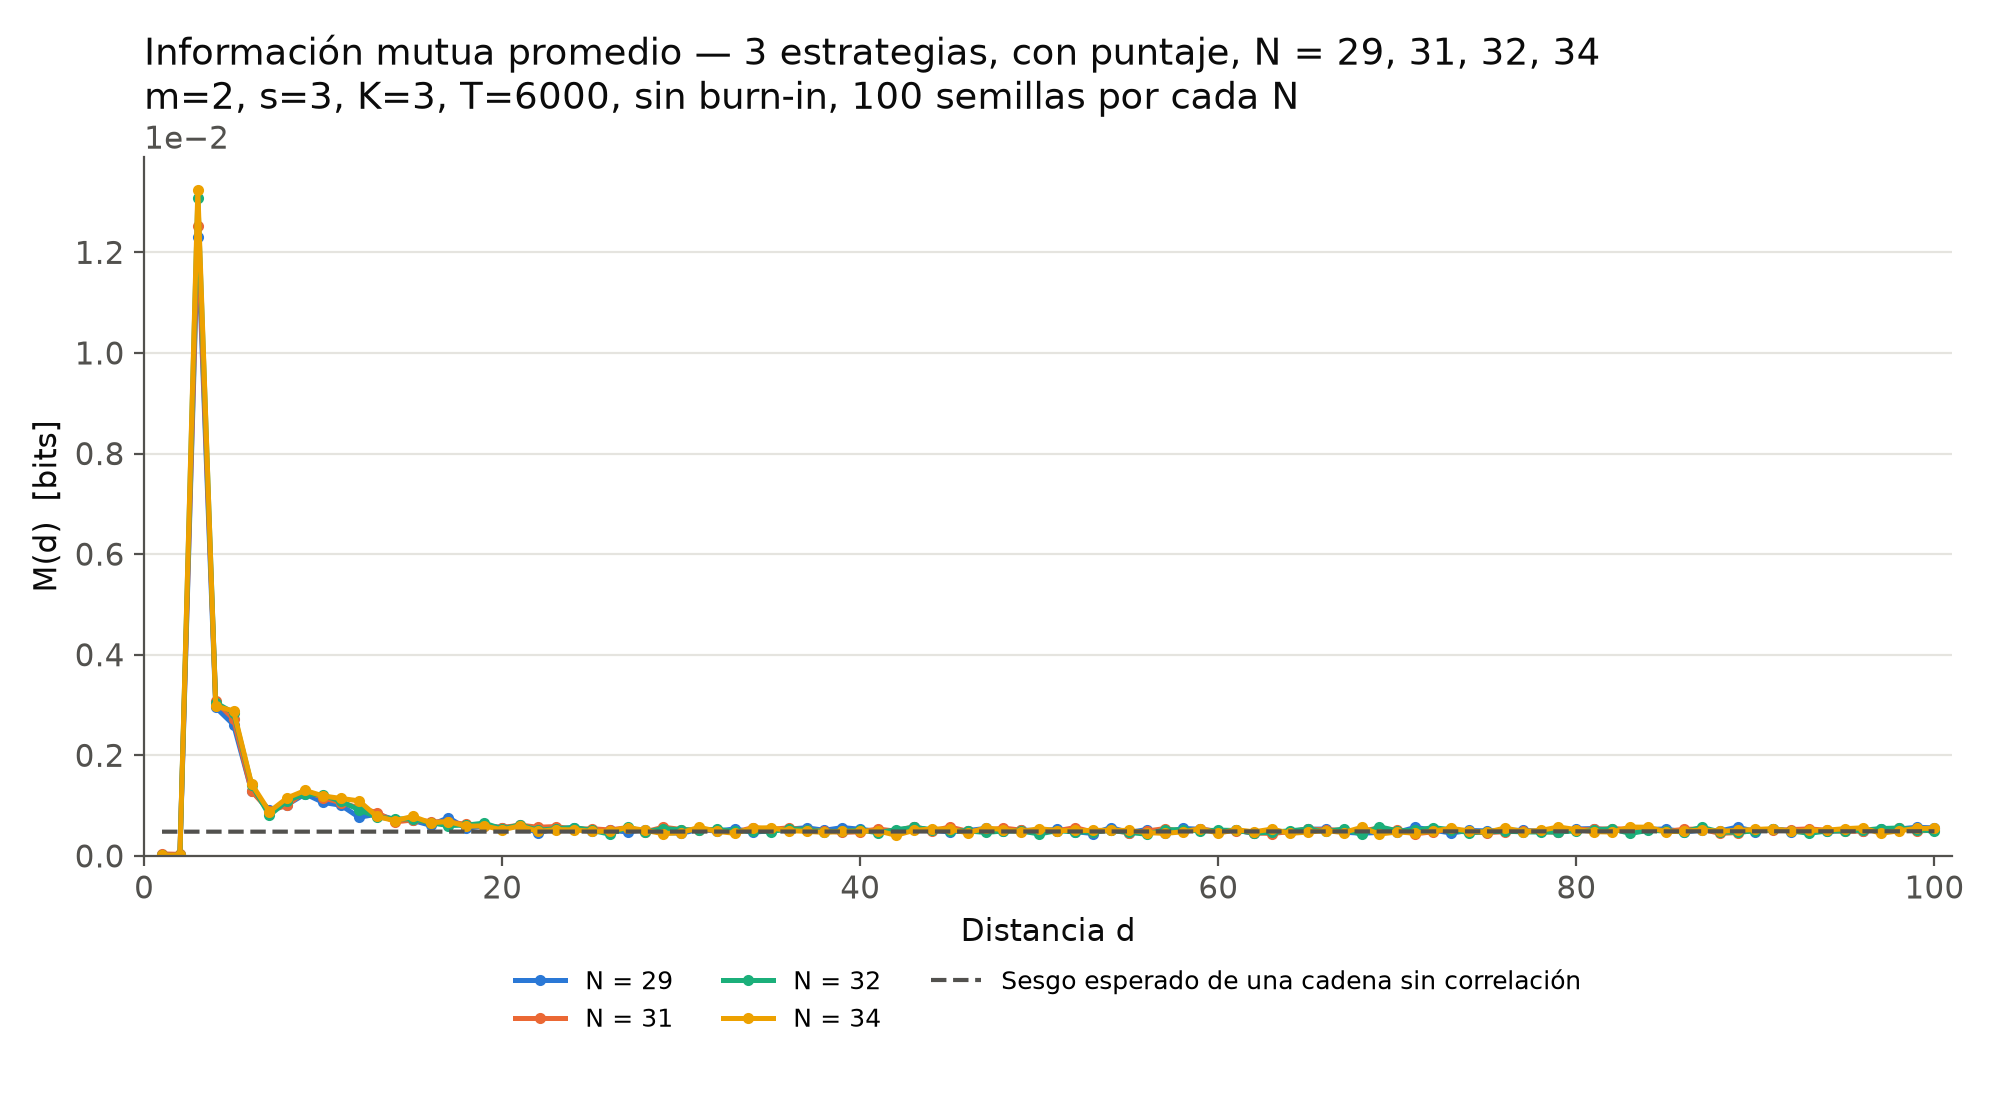
\includegraphics[width=0.49\textwidth]{figuras/Fase6_Md_con_puntaje_m2_s3_T6000_N29-31-32-34_promedio.png}\hfill
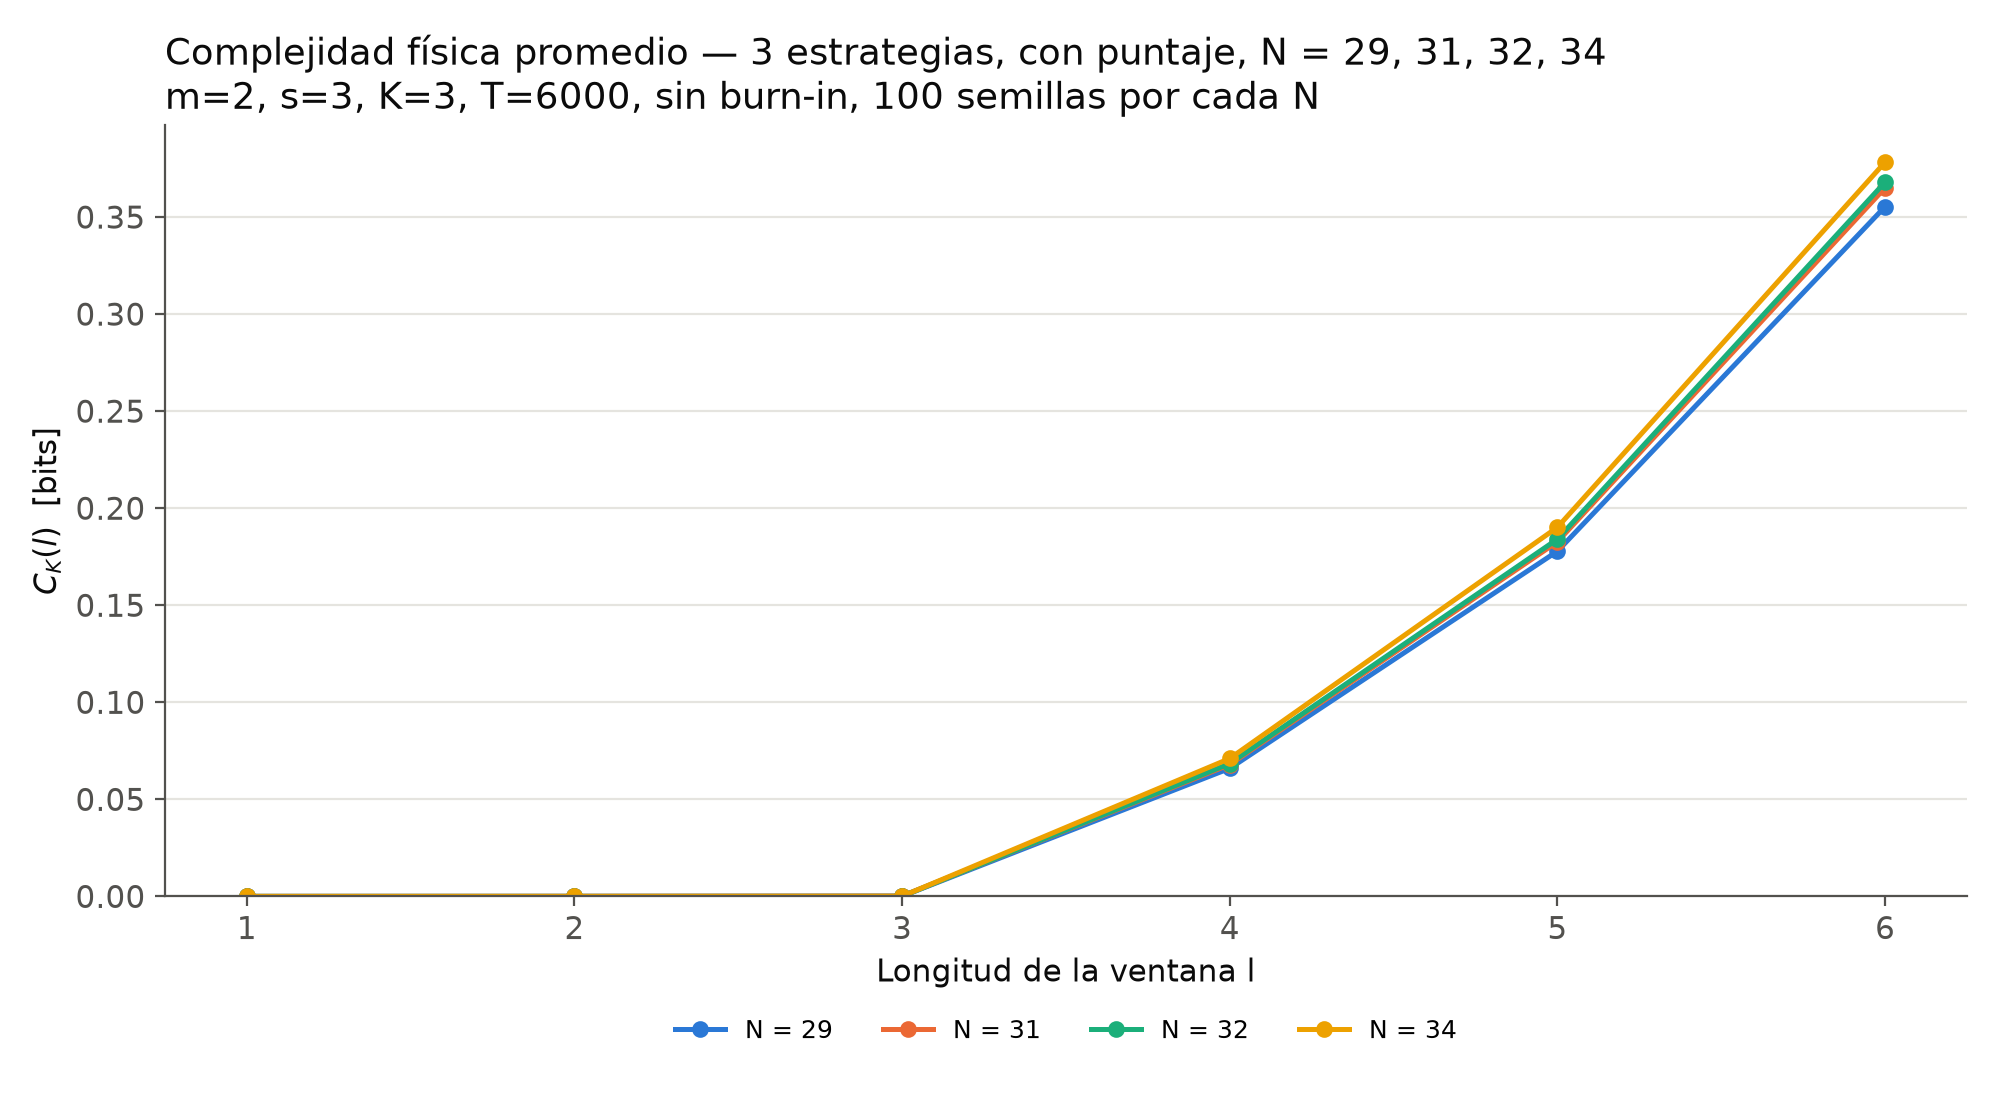
\includegraphics[width=0.49\textwidth]{figuras/Fase6_CK_con_puntaje_m2_s3_T6000_N29-31-32-34_promedio.png}
\caption{Fase 6, $N=29, 31, 32, 34$: $M(d)$ promedio (izquierda) y $C_K(l)$ promedio (derecha).}
\end{figure}
\begin{figure}[H]
\centering
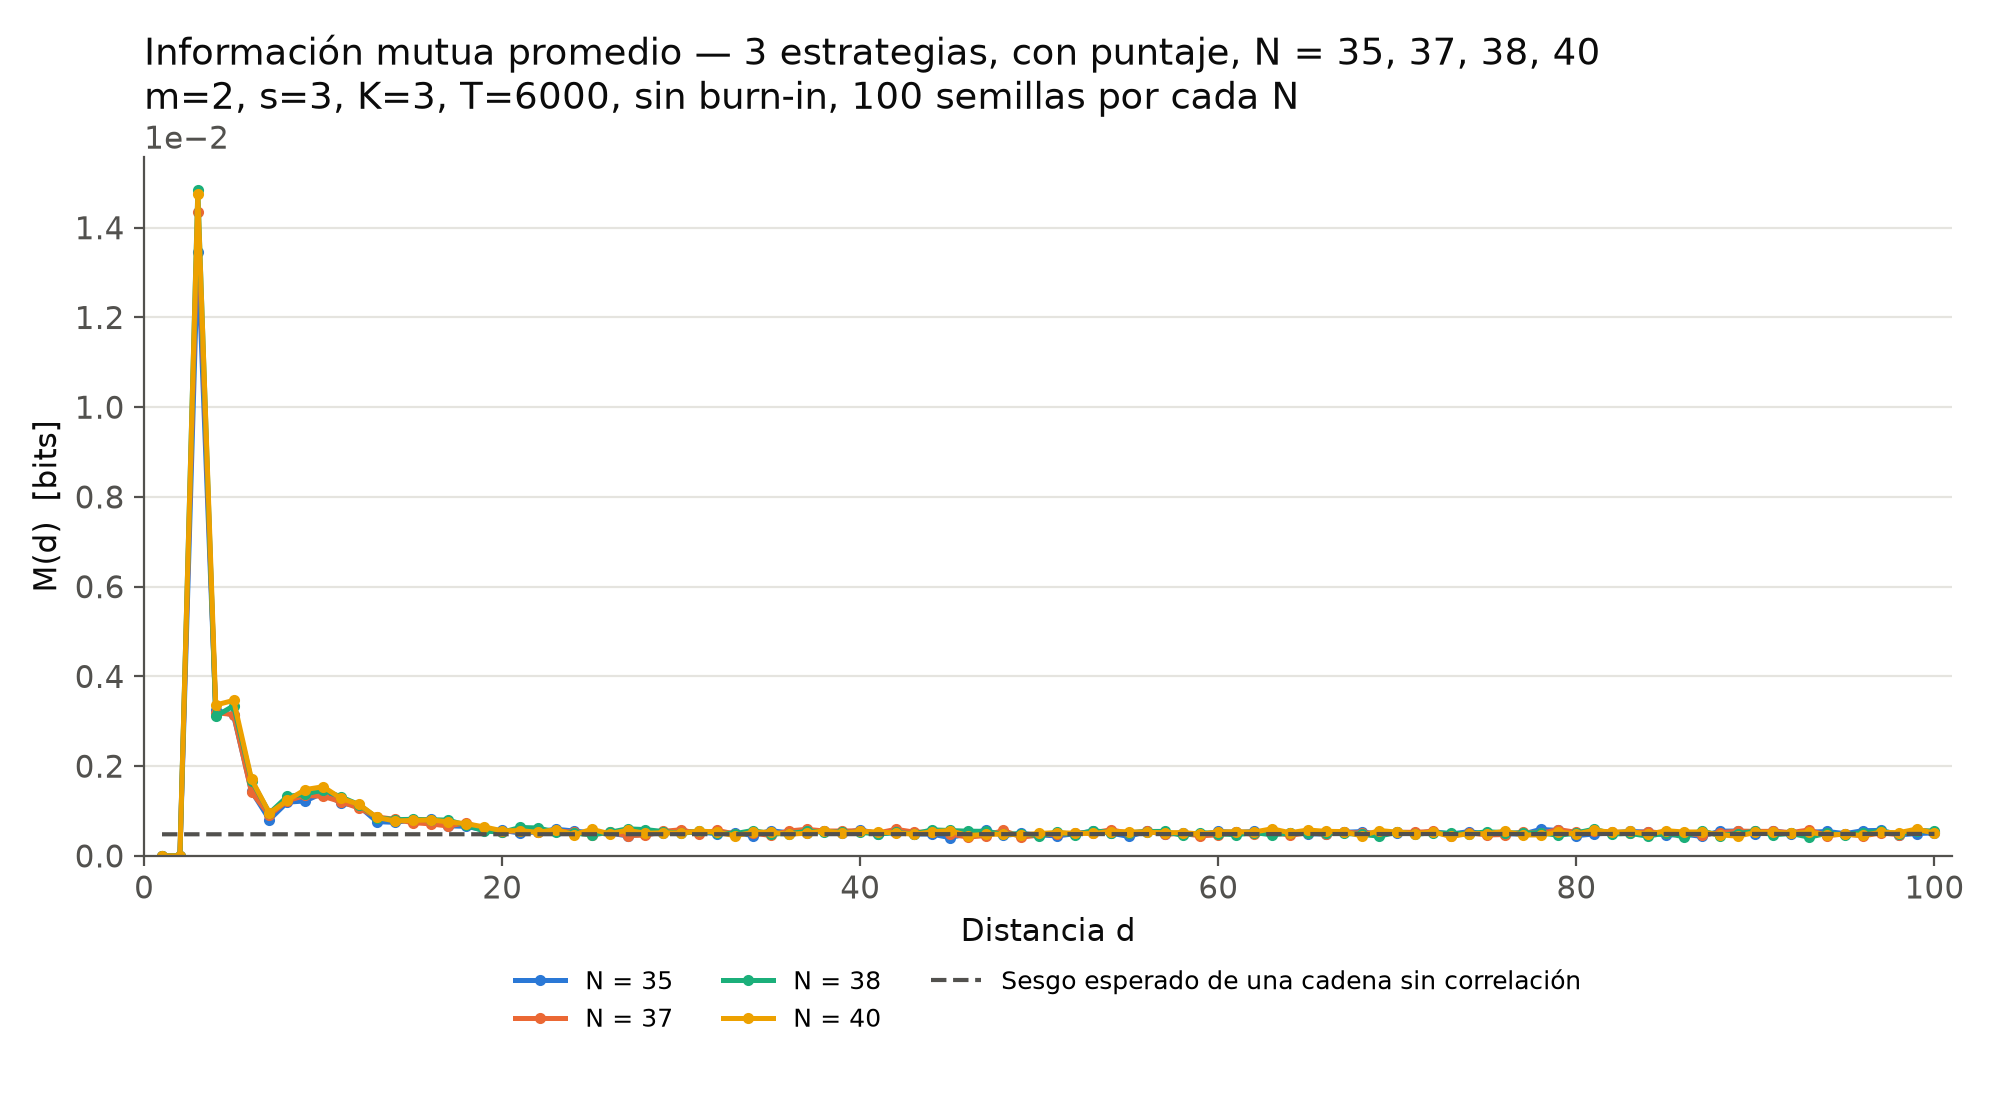
\includegraphics[width=0.49\textwidth]{figuras/Fase6_Md_con_puntaje_m2_s3_T6000_N35-37-38-40_promedio.png}\hfill
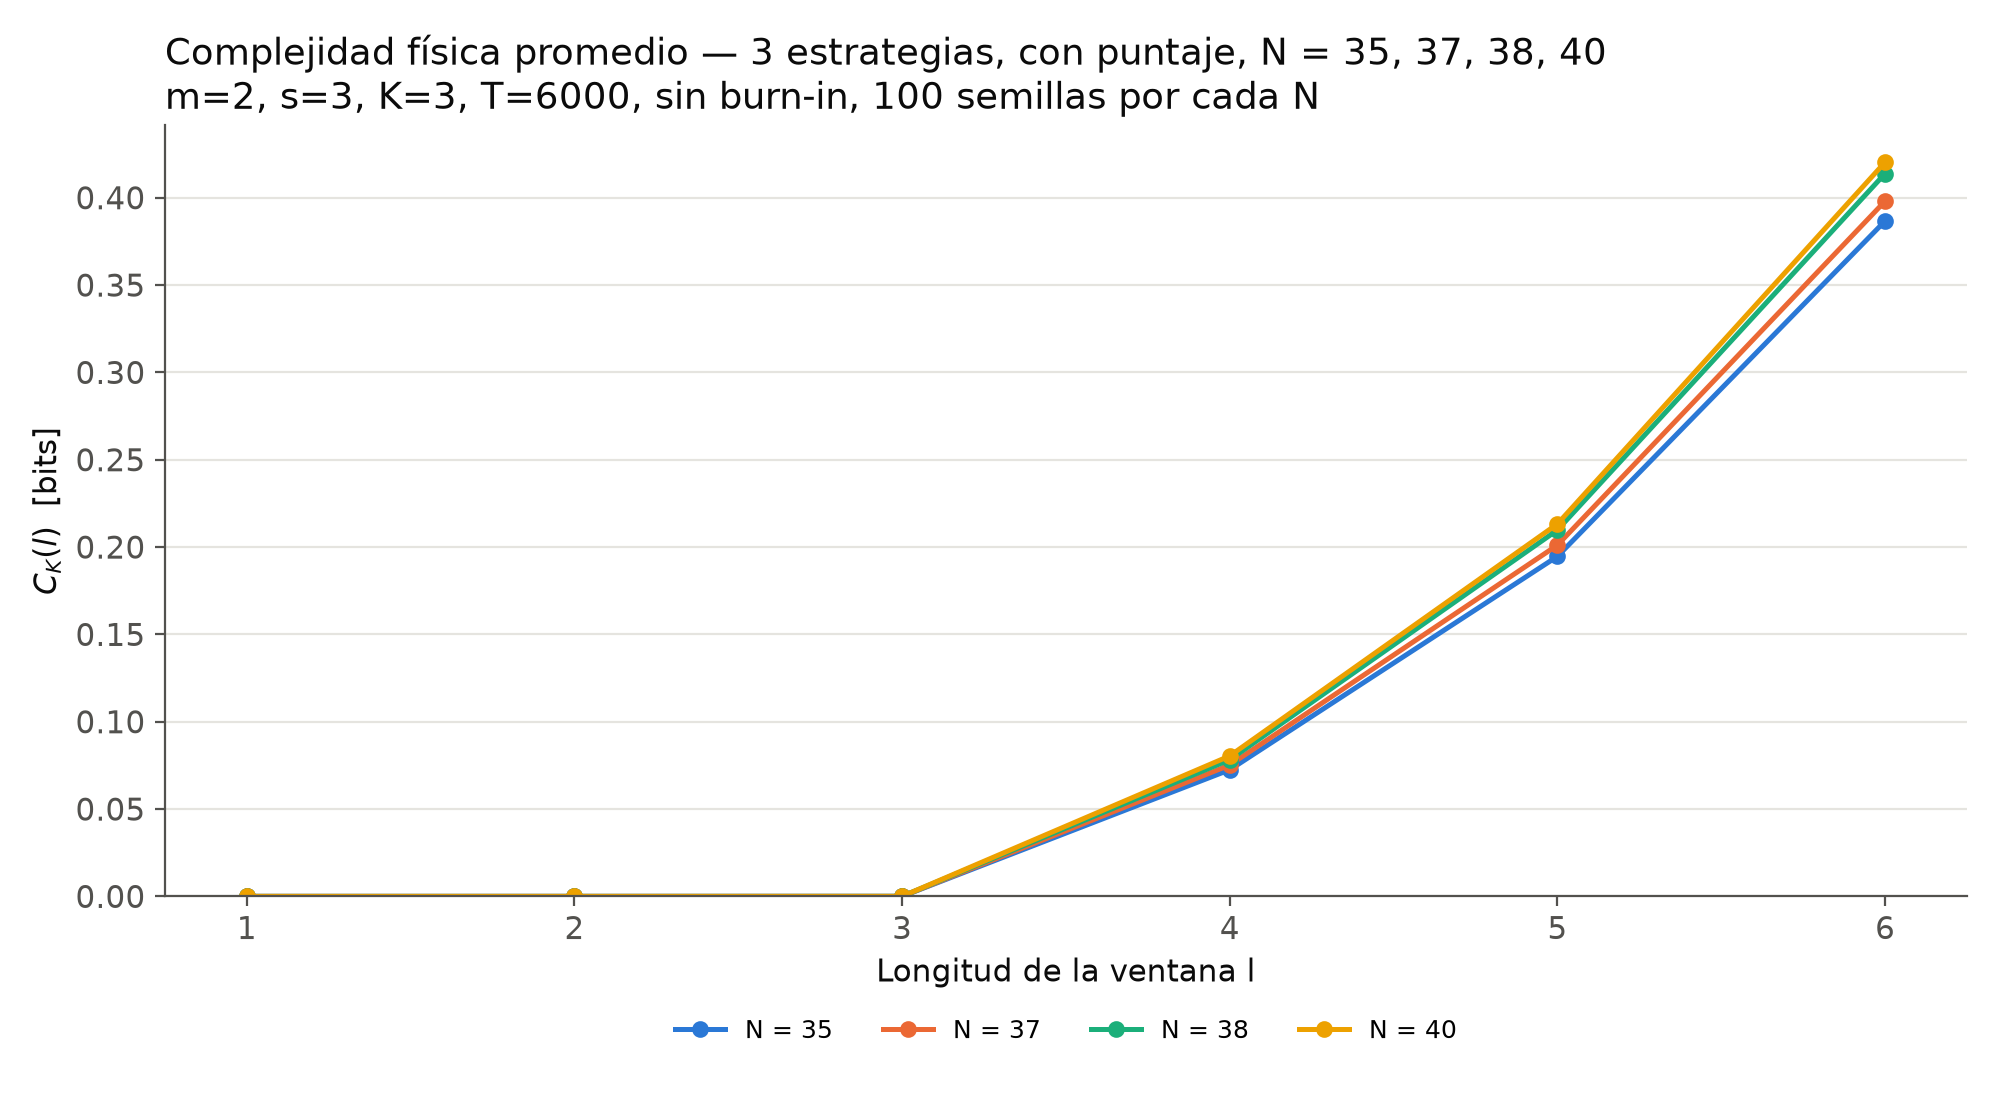
\includegraphics[width=0.49\textwidth]{figuras/Fase6_CK_con_puntaje_m2_s3_T6000_N35-37-38-40_promedio.png}
\caption{Fase 6, $N=35, 37, 38, 40$: $M(d)$ promedio (izquierda) y $C_K(l)$ promedio (derecha).}
\end{figure}
\begin{figure}[H]
\centering
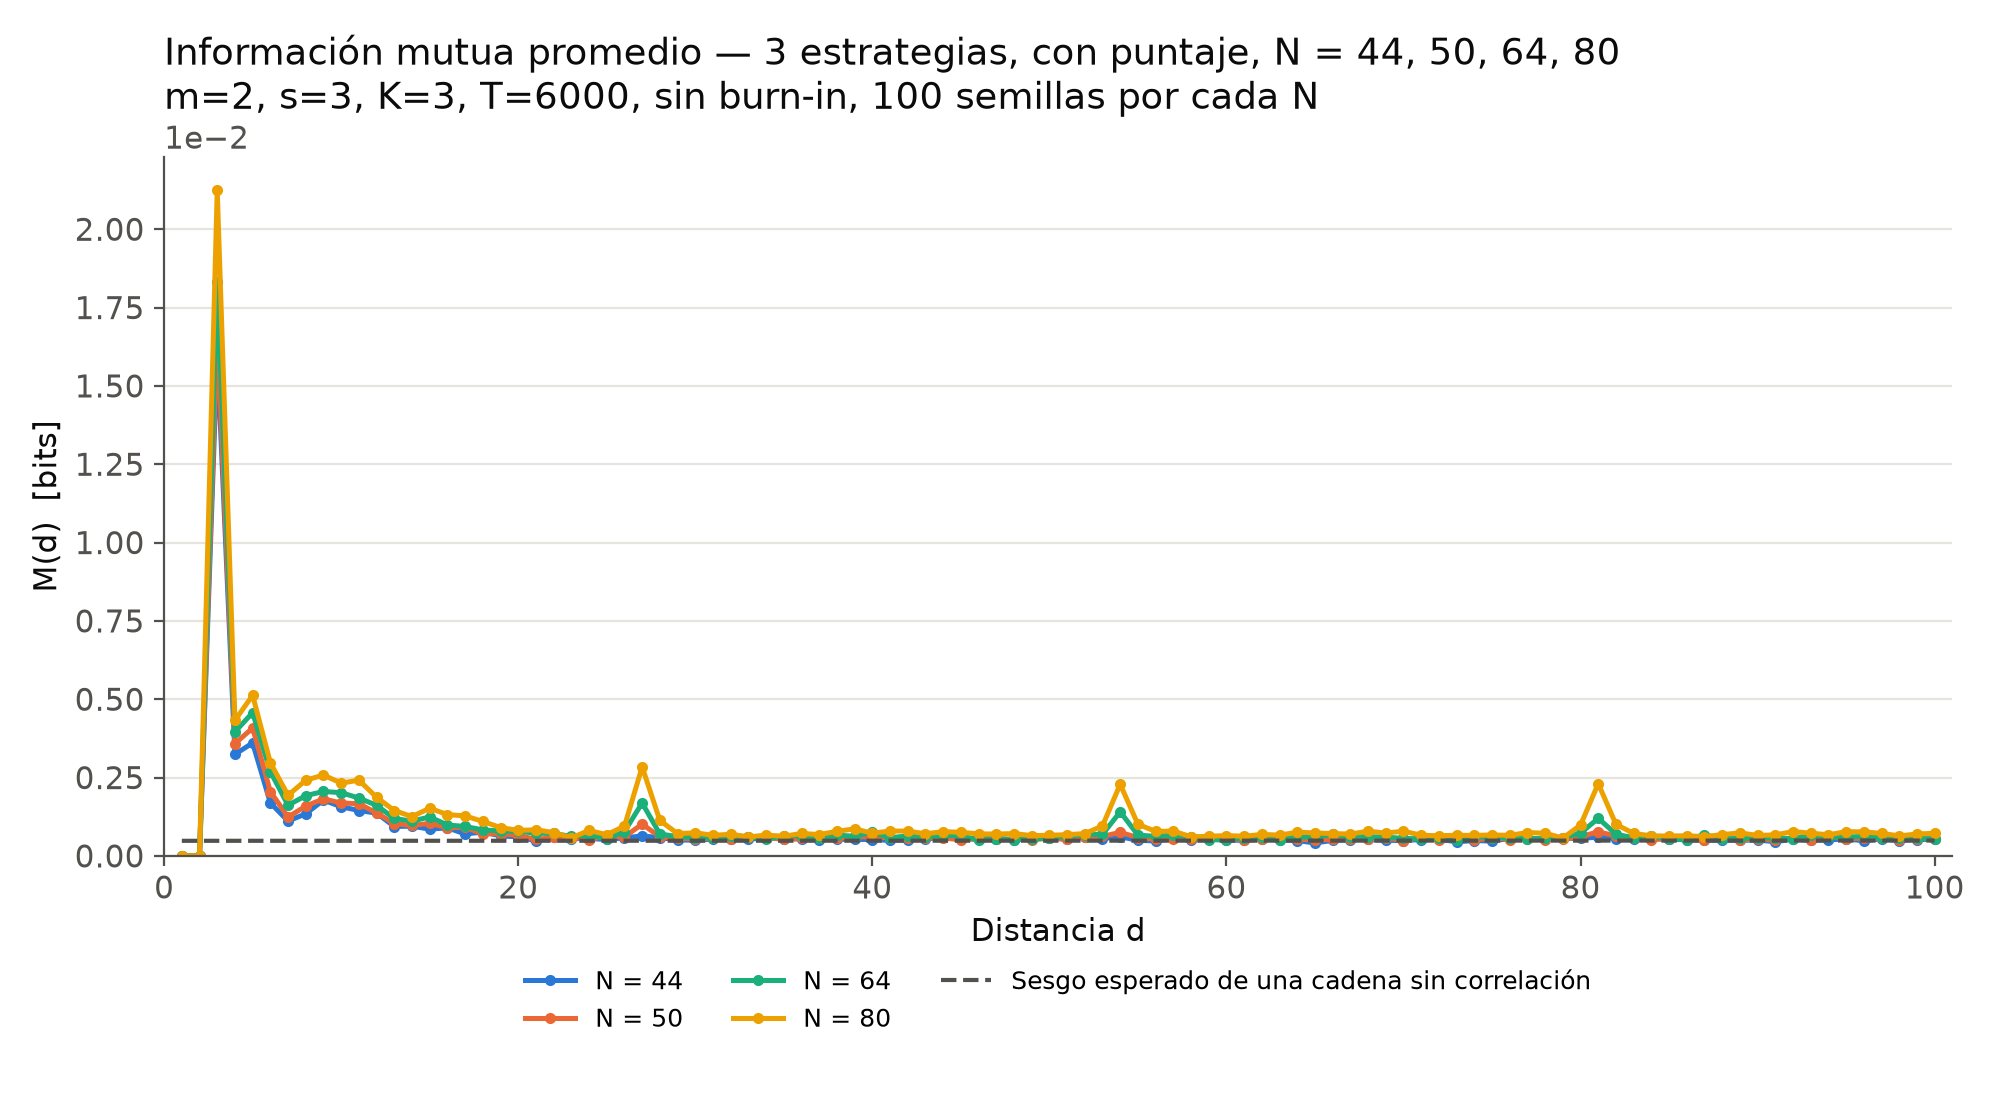
\includegraphics[width=0.49\textwidth]{figuras/Fase6_Md_con_puntaje_m2_s3_T6000_N44-50-64-80_promedio.png}\hfill
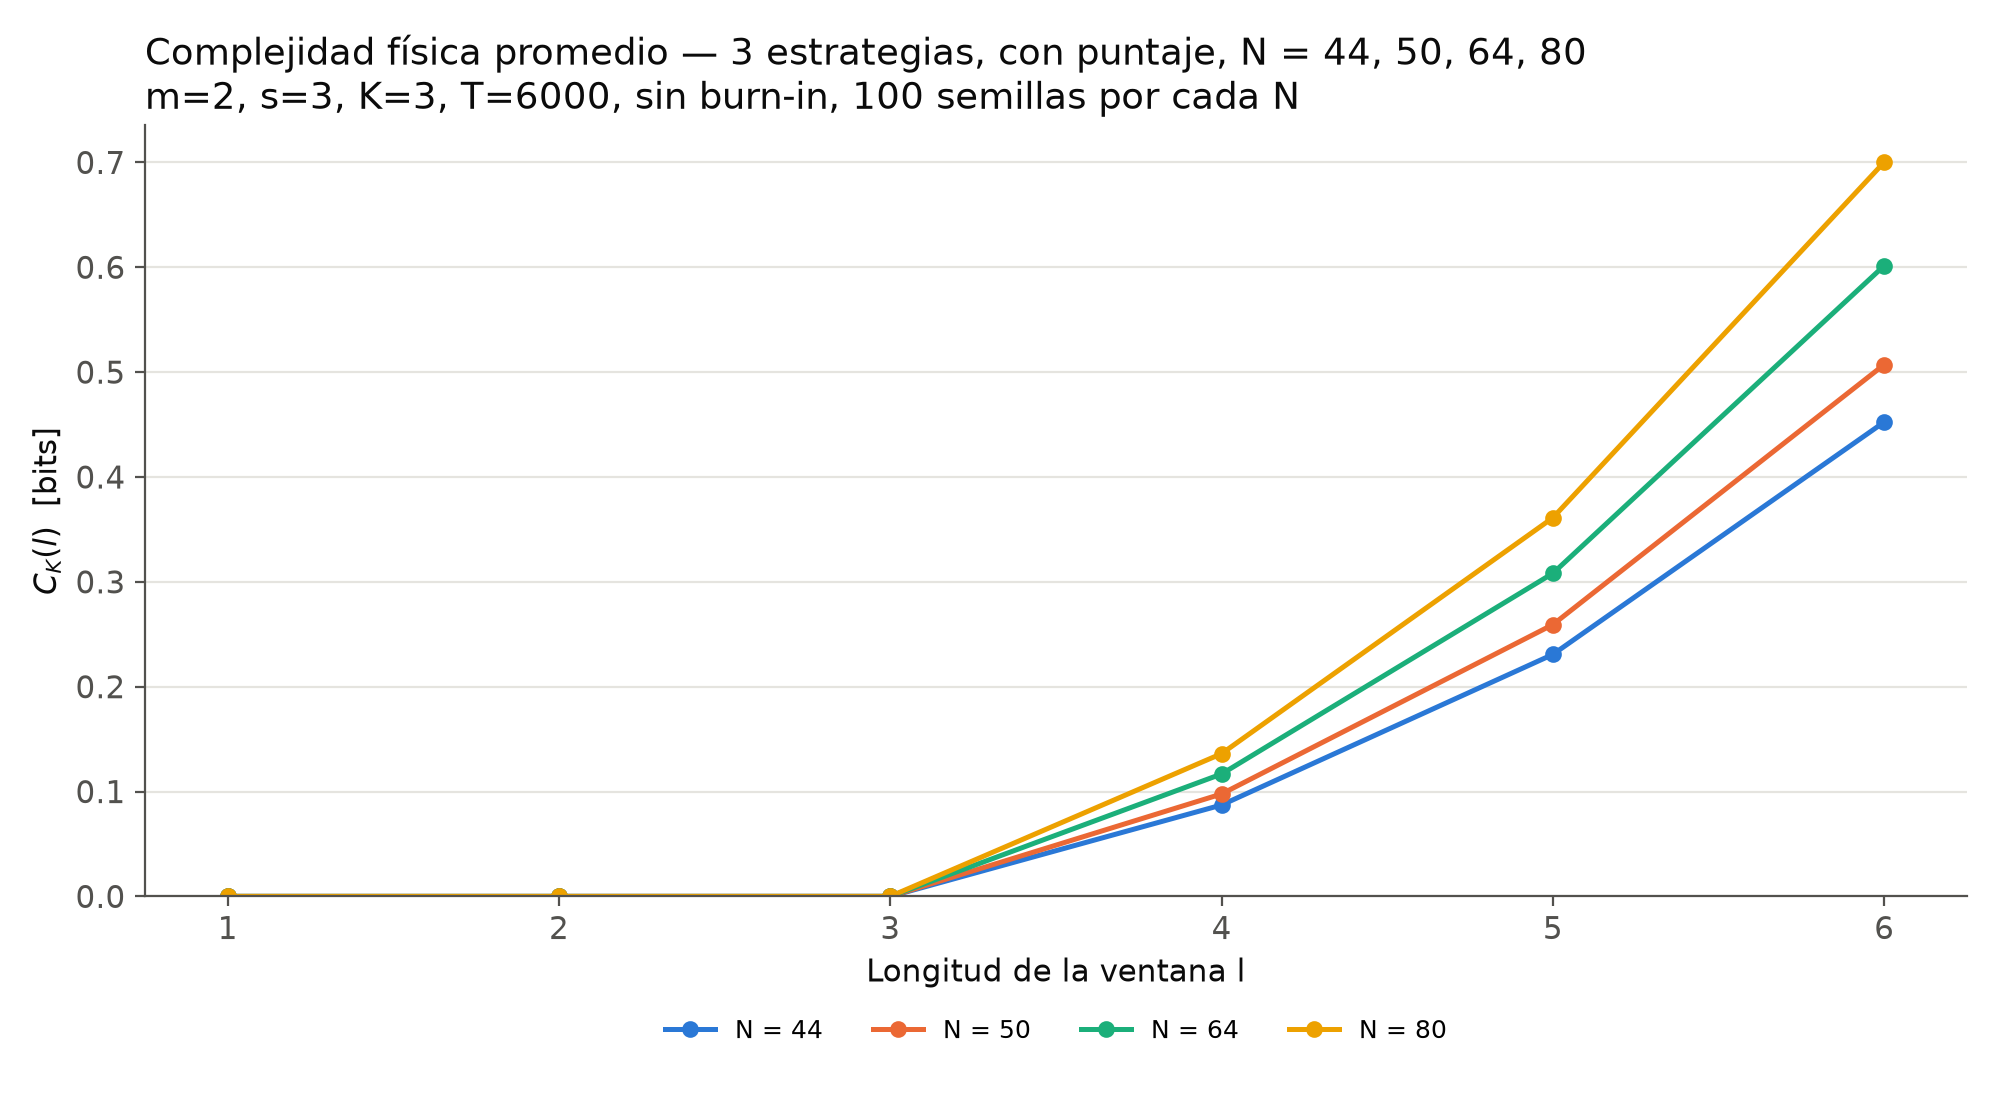
\includegraphics[width=0.49\textwidth]{figuras/Fase6_CK_con_puntaje_m2_s3_T6000_N44-50-64-80_promedio.png}
\caption{Fase 6, $N=44, 50, 64, 80$: $M(d)$ promedio (izquierda) y $C_K(l)$ promedio (derecha).}
\end{figure}
\begin{figure}[H]
\centering
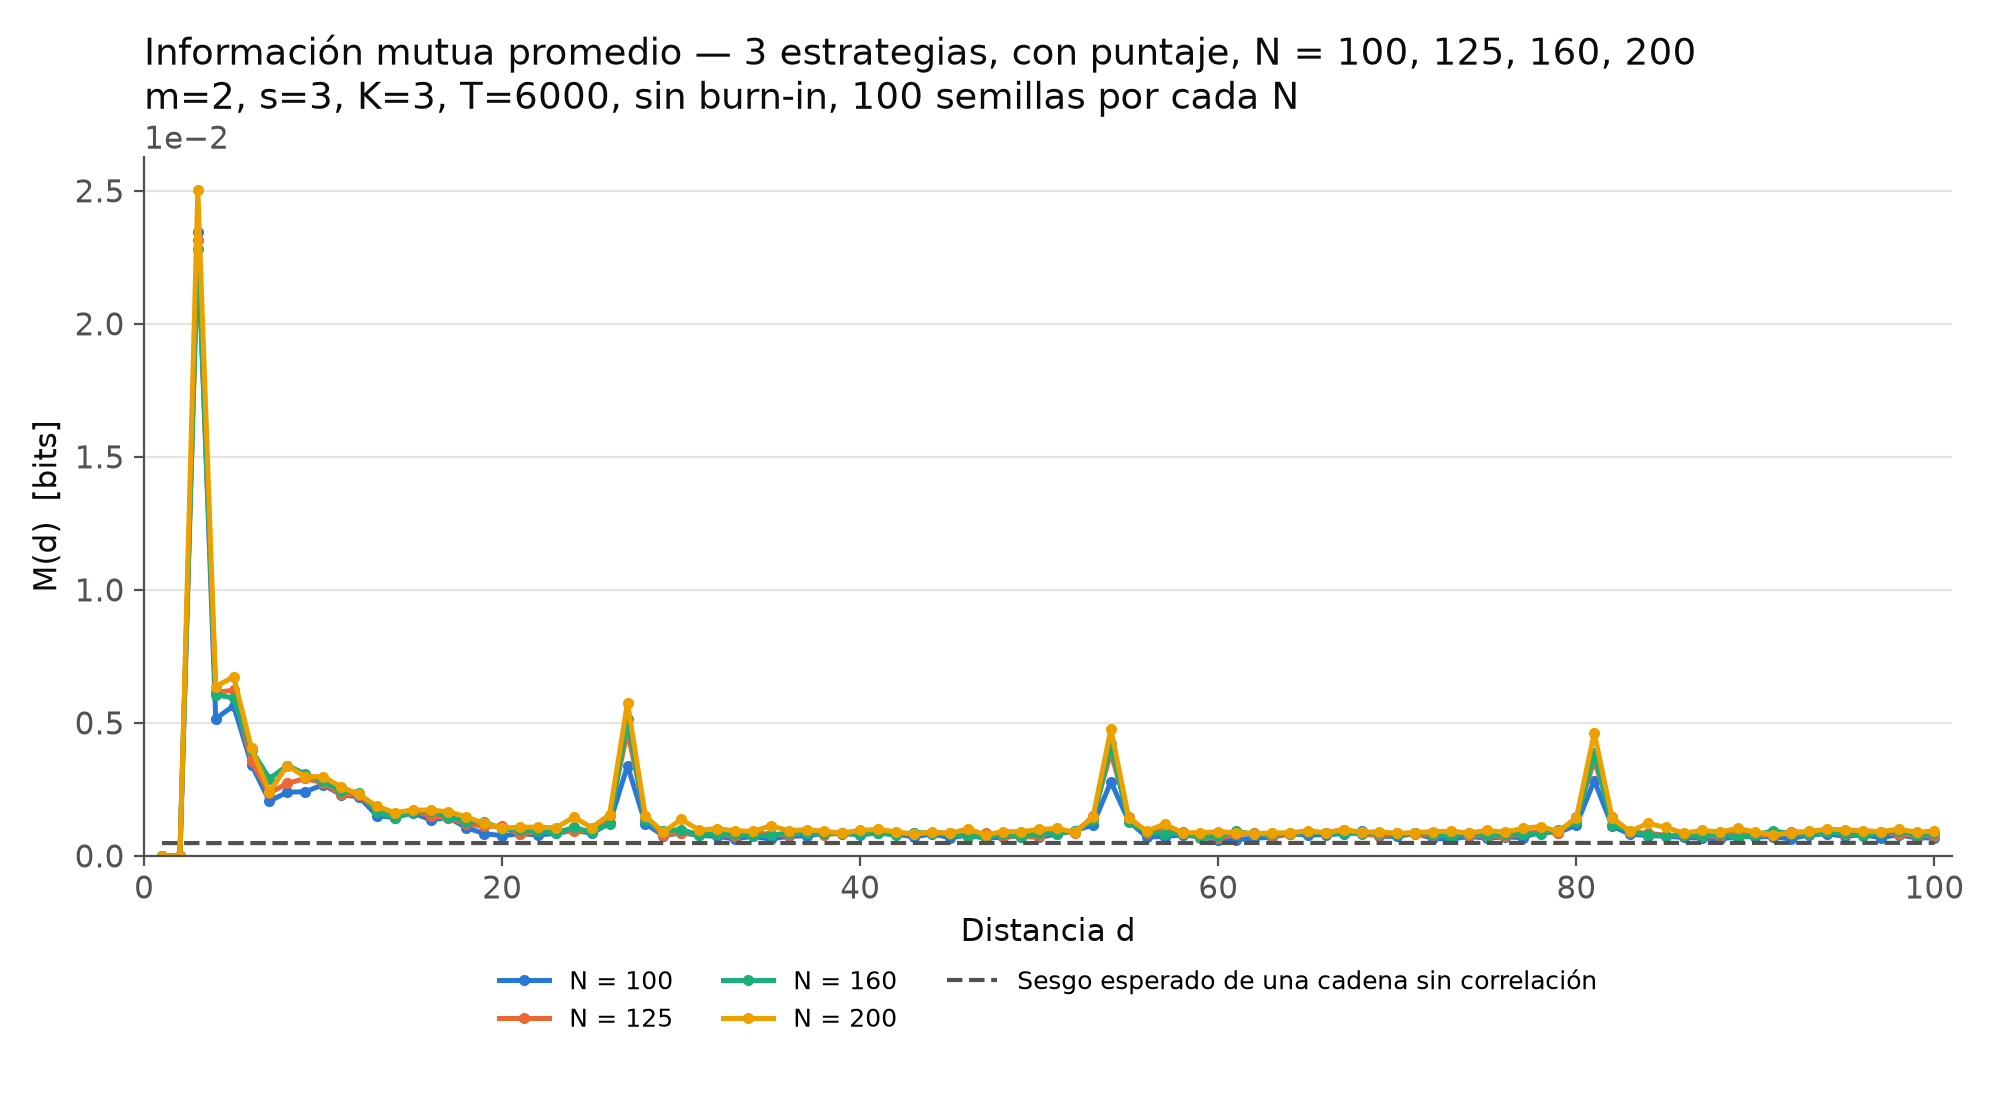
\includegraphics[width=0.49\textwidth]{figuras/Fase6_Md_con_puntaje_m2_s3_T6000_N100-125-160-200_promedio.png}\hfill
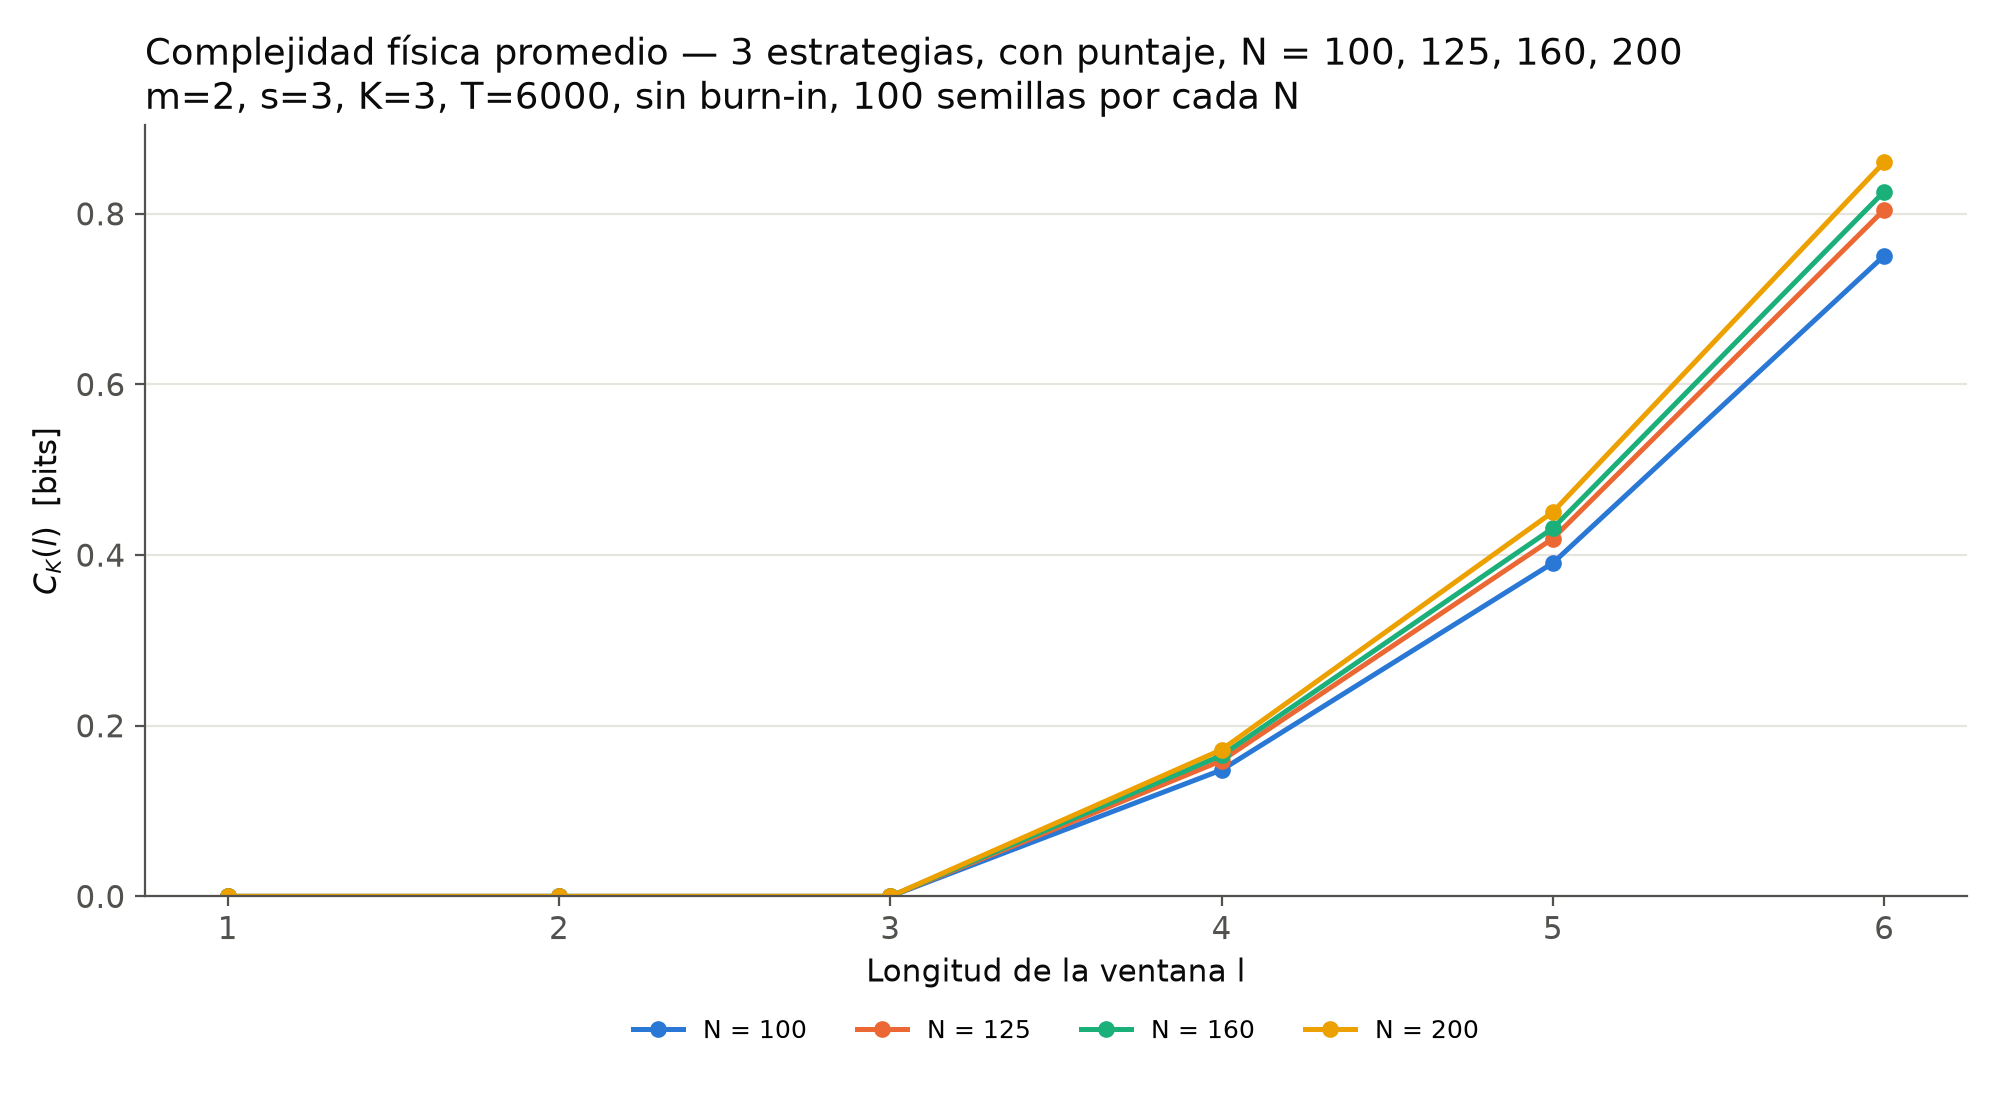
\includegraphics[width=0.49\textwidth]{figuras/Fase6_CK_con_puntaje_m2_s3_T6000_N100-125-160-200_promedio.png}
\caption{Fase 6, $N=100, 125, 160, 200$: $M(d)$ promedio (izquierda) y $C_K(l)$ promedio (derecha).}
\end{figure}
\begin{figure}[H]
\centering
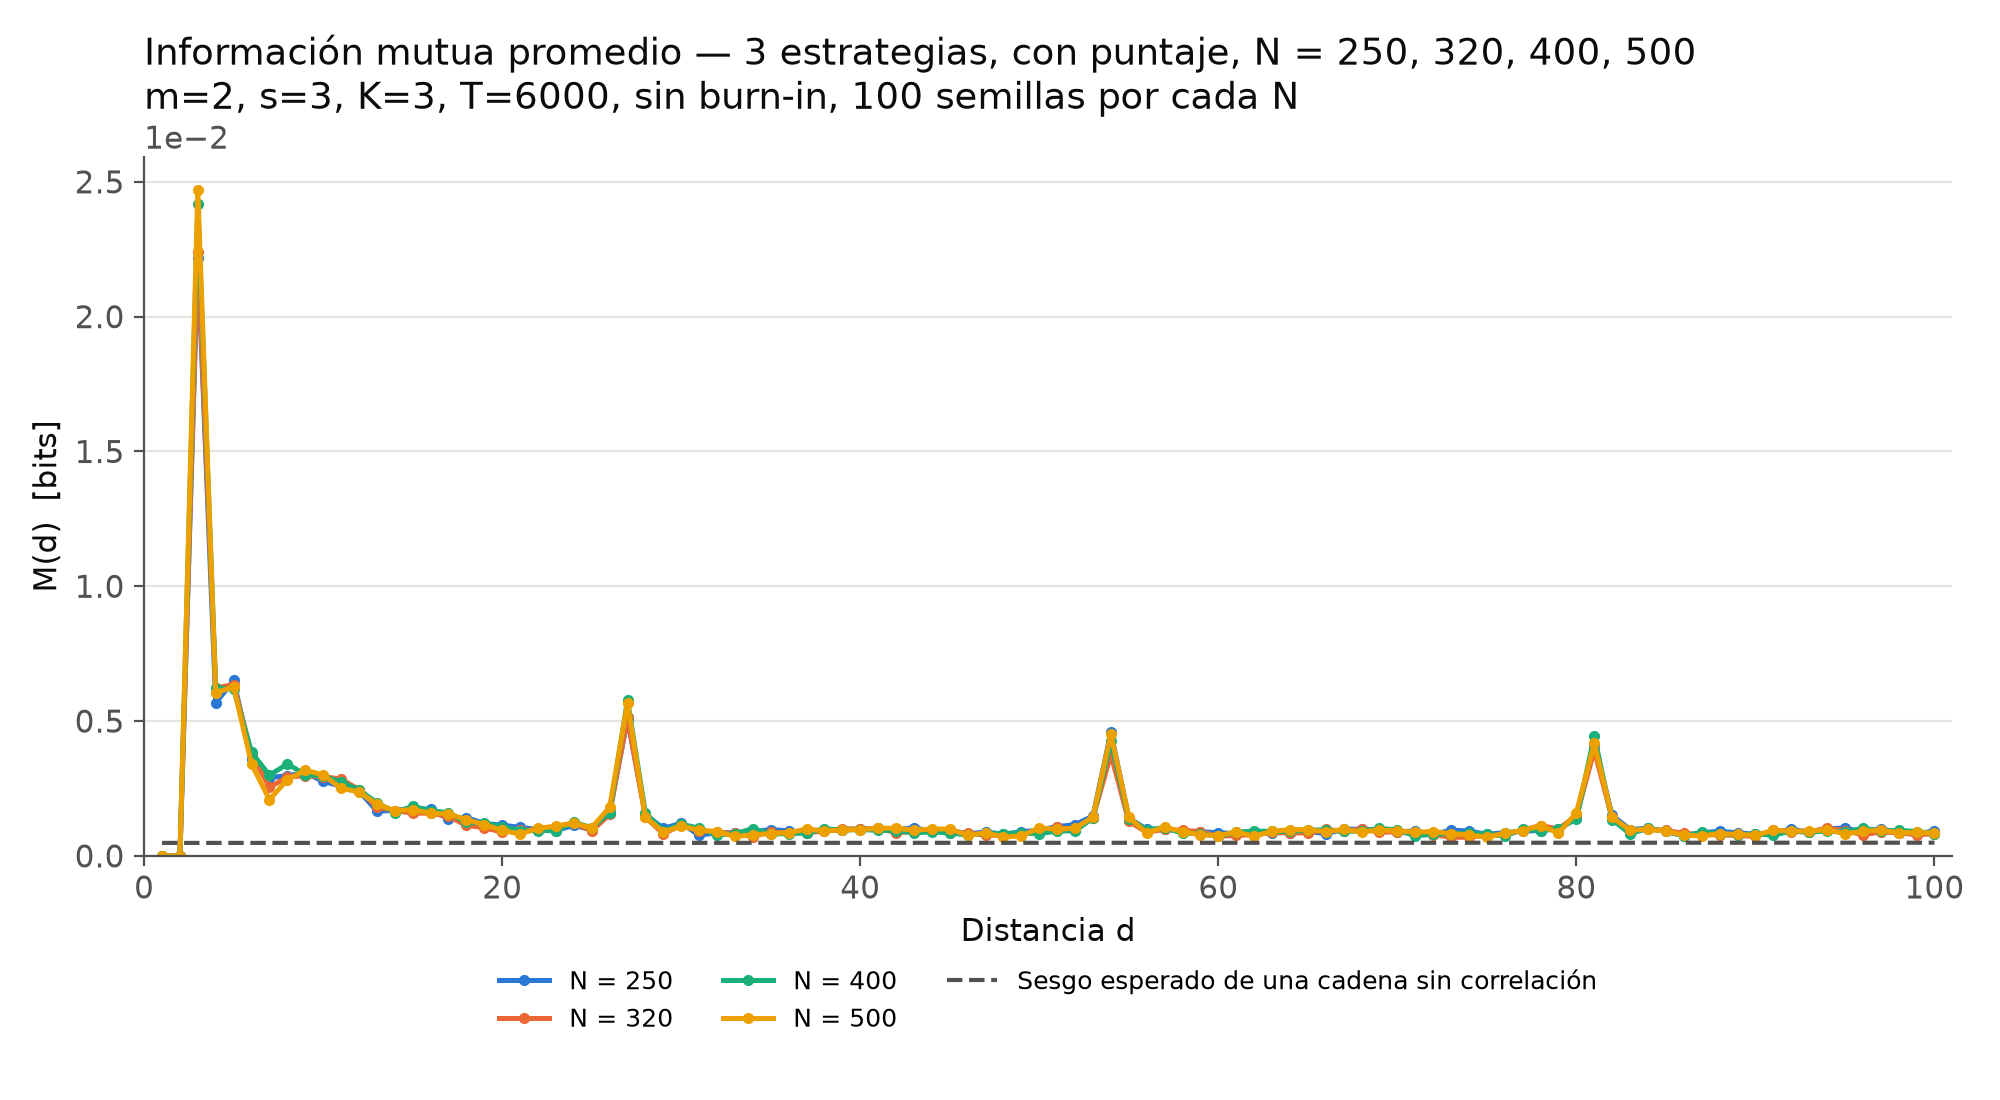
\includegraphics[width=0.49\textwidth]{figuras/Fase6_Md_con_puntaje_m2_s3_T6000_N250-320-400-500_promedio.png}\hfill
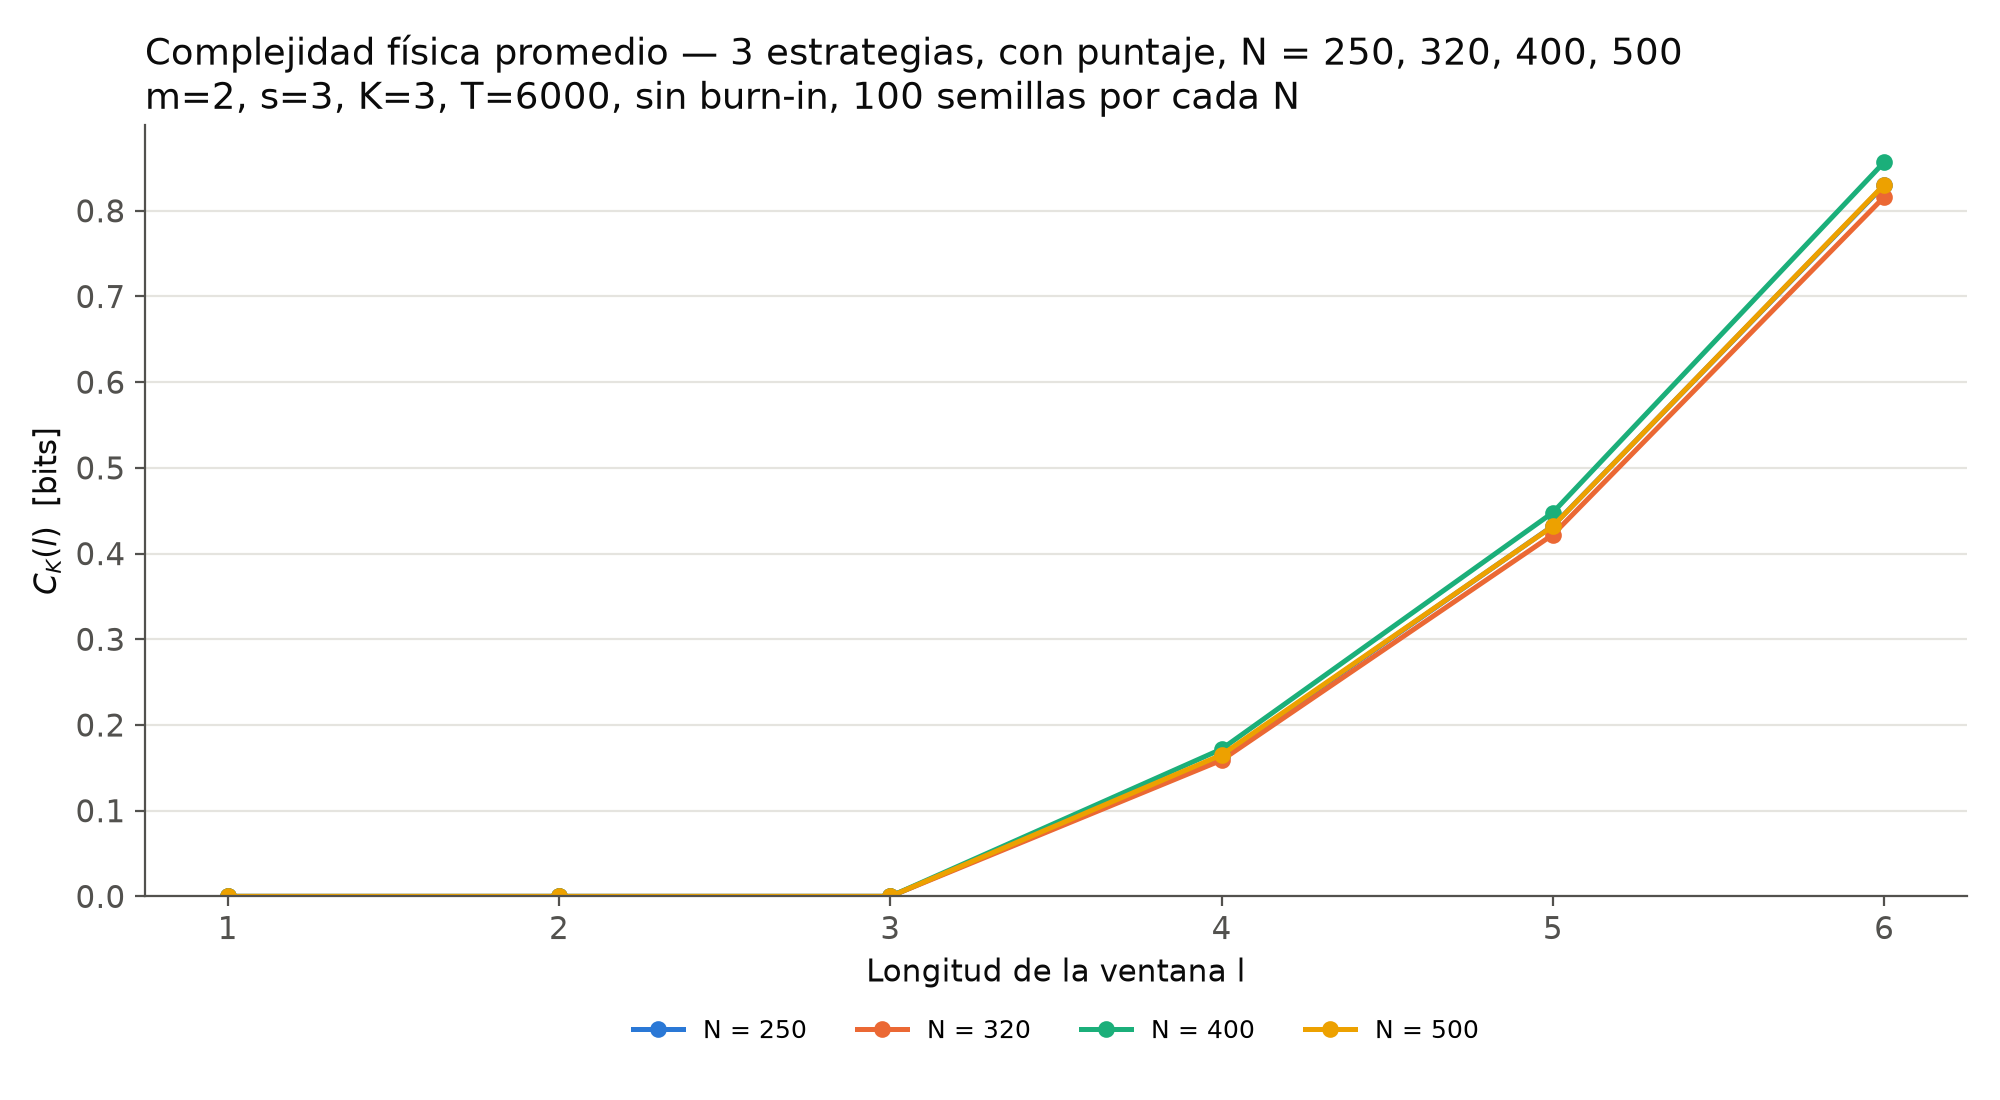
\includegraphics[width=0.49\textwidth]{figuras/Fase6_CK_con_puntaje_m2_s3_T6000_N250-320-400-500_promedio.png}
\caption{Fase 6, $N=250, 320, 400, 500$: $M(d)$ promedio (izquierda) y $C_K(l)$ promedio (derecha).}
\end{figure}
\begin{figure}[H]
\centering
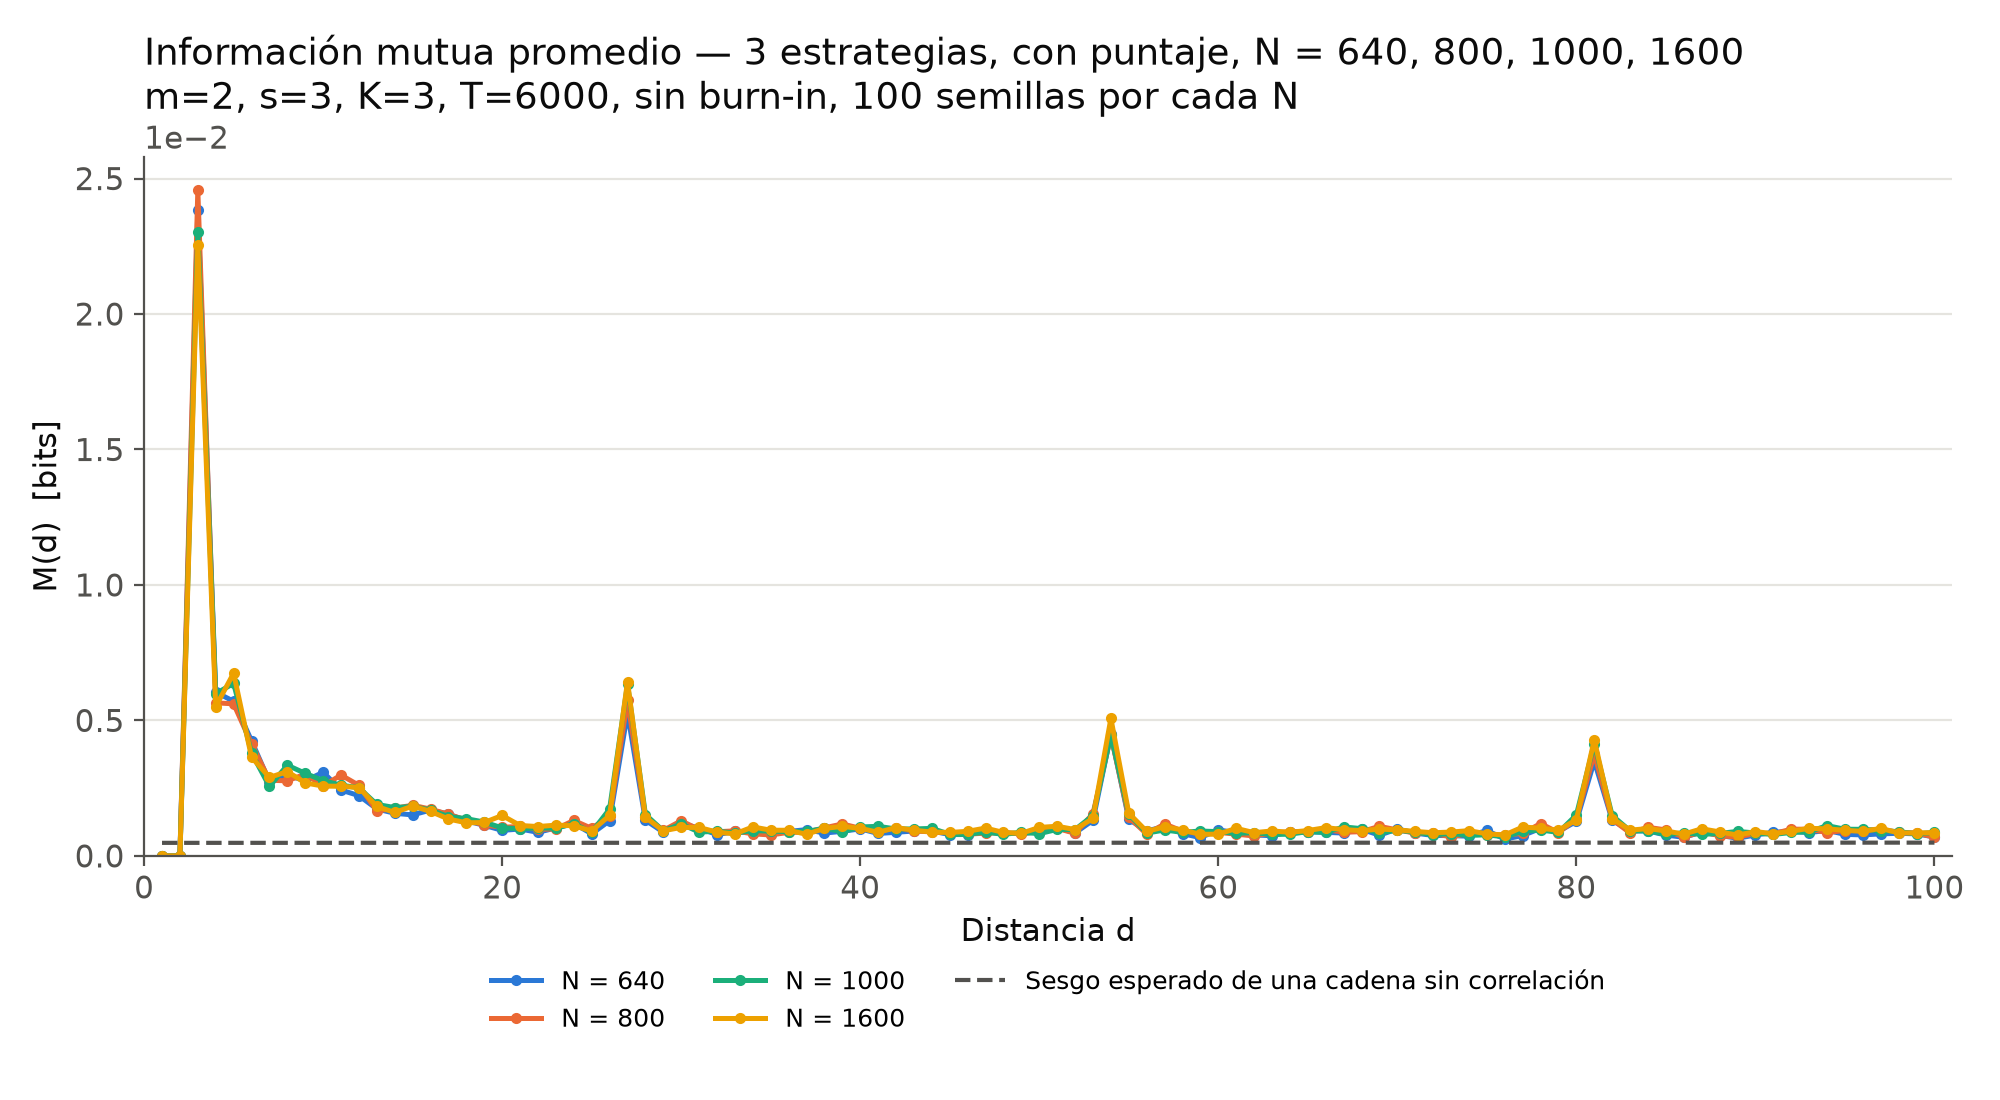
\includegraphics[width=0.49\textwidth]{figuras/Fase6_Md_con_puntaje_m2_s3_T6000_N640-800-1000-1600_promedio.png}\hfill
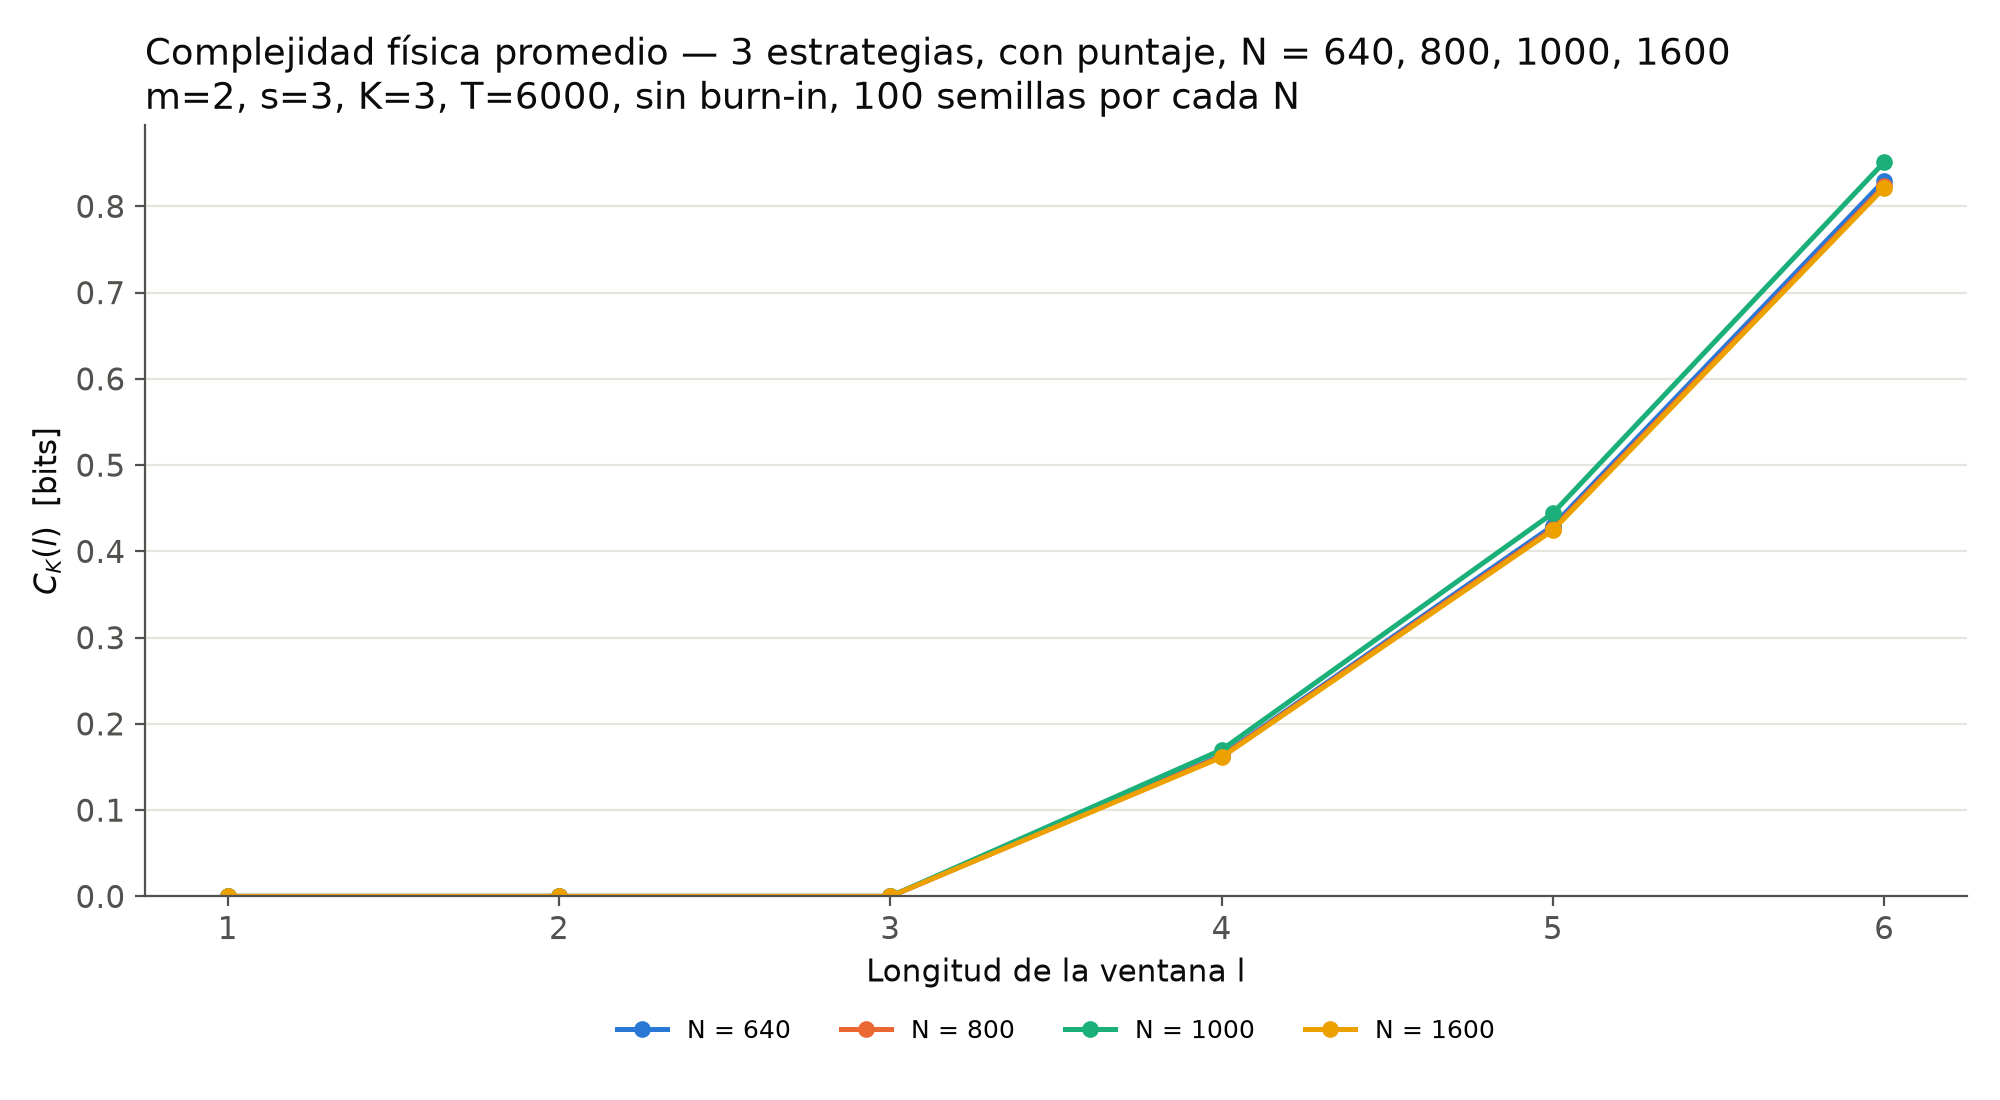
\includegraphics[width=0.49\textwidth]{figuras/Fase6_CK_con_puntaje_m2_s3_T6000_N640-800-1000-1600_promedio.png}
\caption{Fase 6, $N=640, 800, 1000, 1600$: $M(d)$ promedio (izquierda) y $C_K(l)$ promedio (derecha).}
\end{figure}
\begin{figure}[H]
\centering
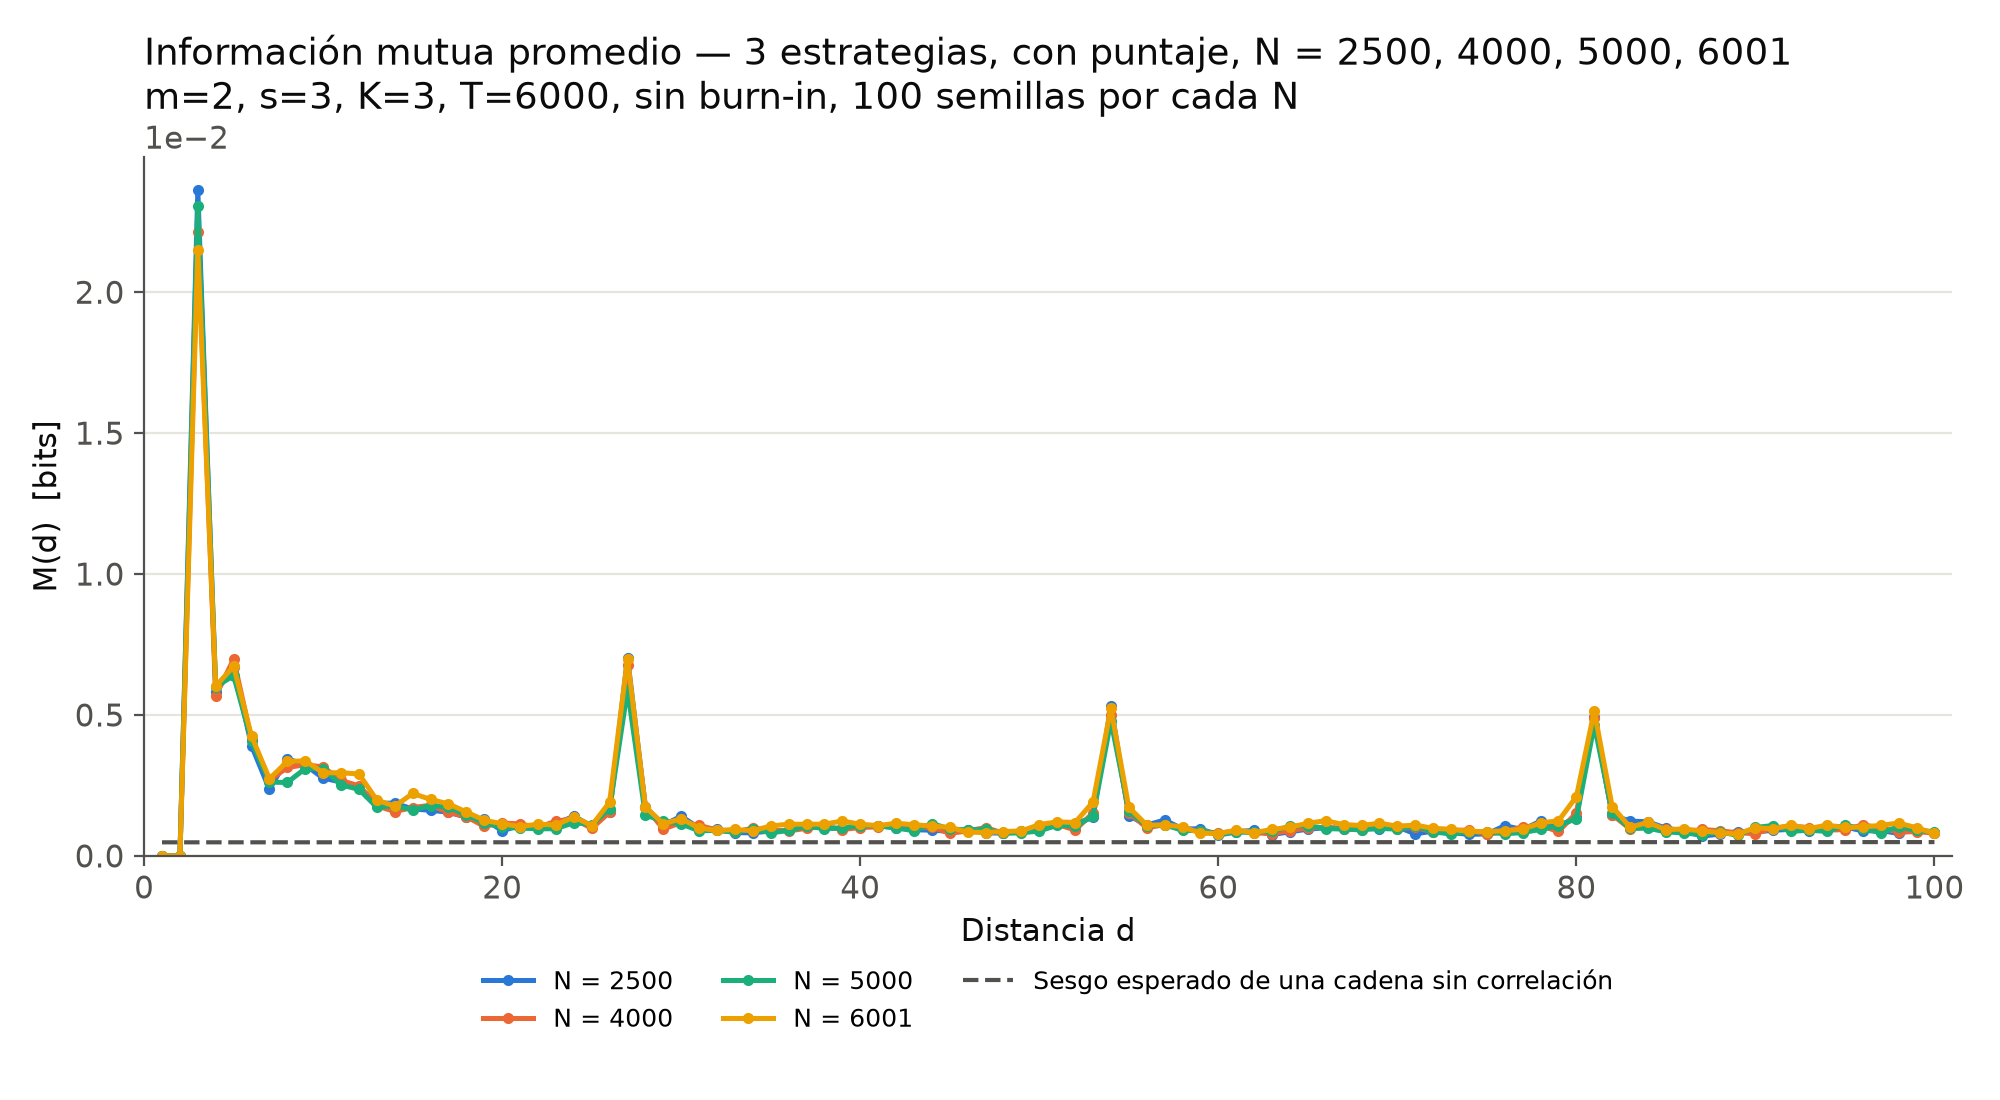
\includegraphics[width=0.49\textwidth]{figuras/Fase6_Md_con_puntaje_m2_s3_T6000_N2500-4000-5000-6001_promedio.png}\hfill
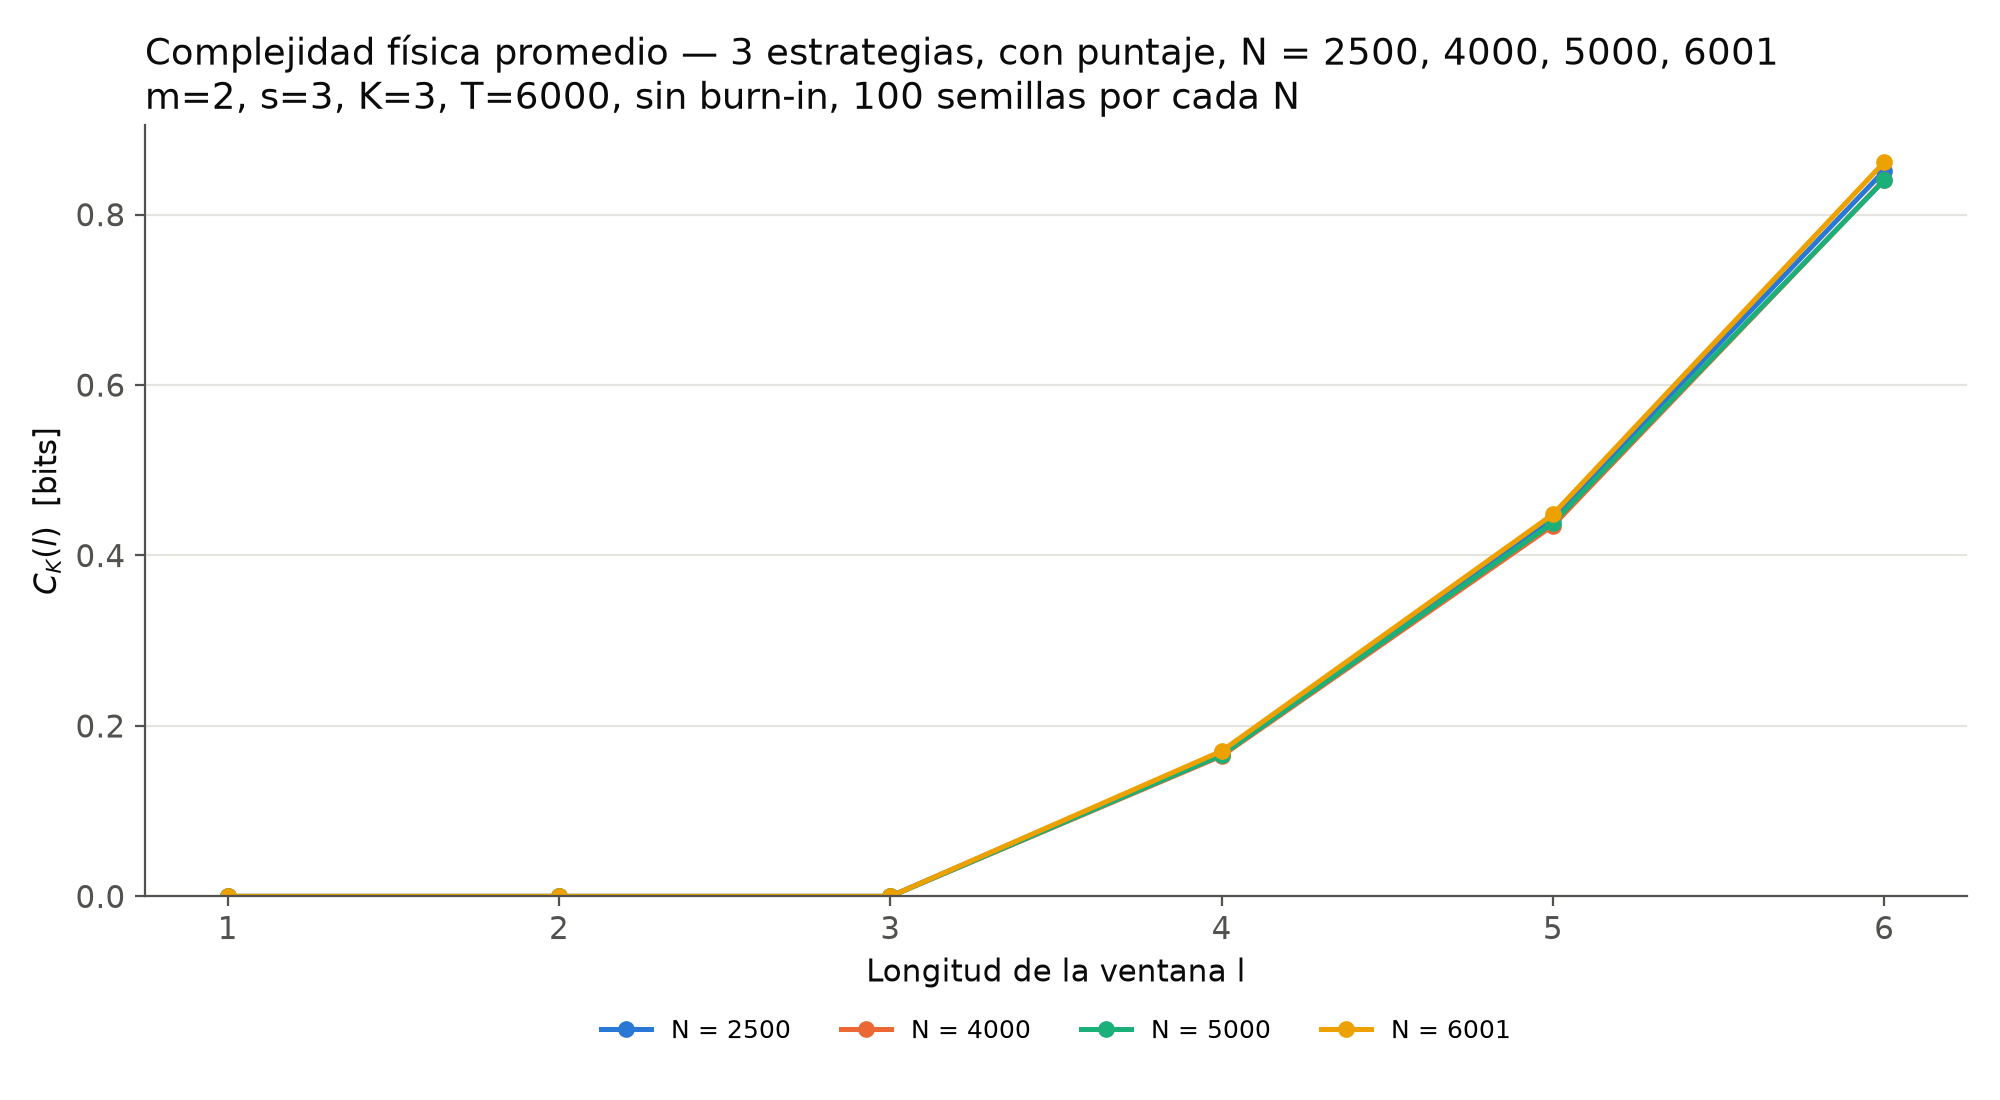
\includegraphics[width=0.49\textwidth]{figuras/Fase6_CK_con_puntaje_m2_s3_T6000_N2500-4000-5000-6001_promedio.png}
\caption{Fase 6, $N=2500, 4000, 5000, 6001$: $M(d)$ promedio (izquierda) y $C_K(l)$ promedio (derecha).}
\end{figure}
\begin{figure}[H]
\centering
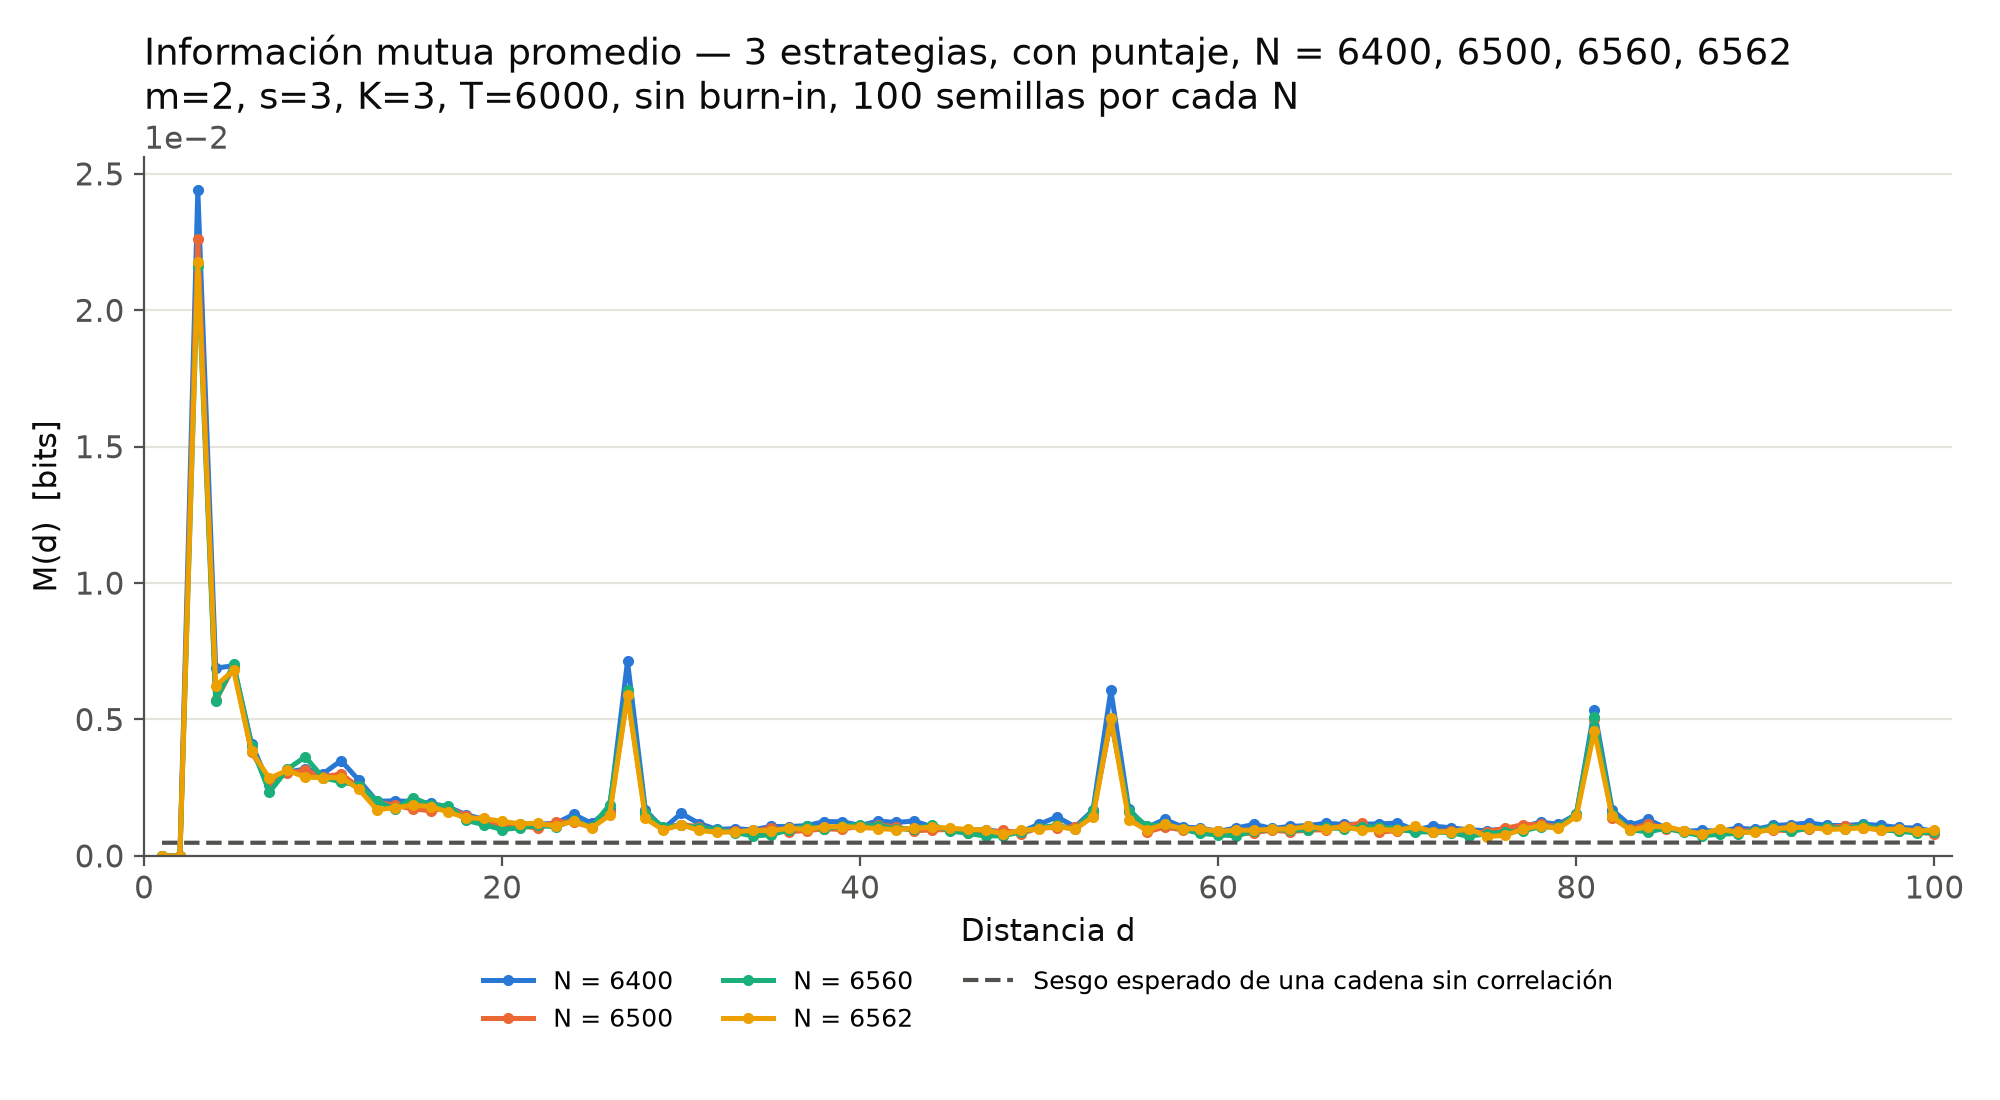
\includegraphics[width=0.49\textwidth]{figuras/Fase6_Md_con_puntaje_m2_s3_T6000_N6400-6500-6560-6562_promedio.png}\hfill
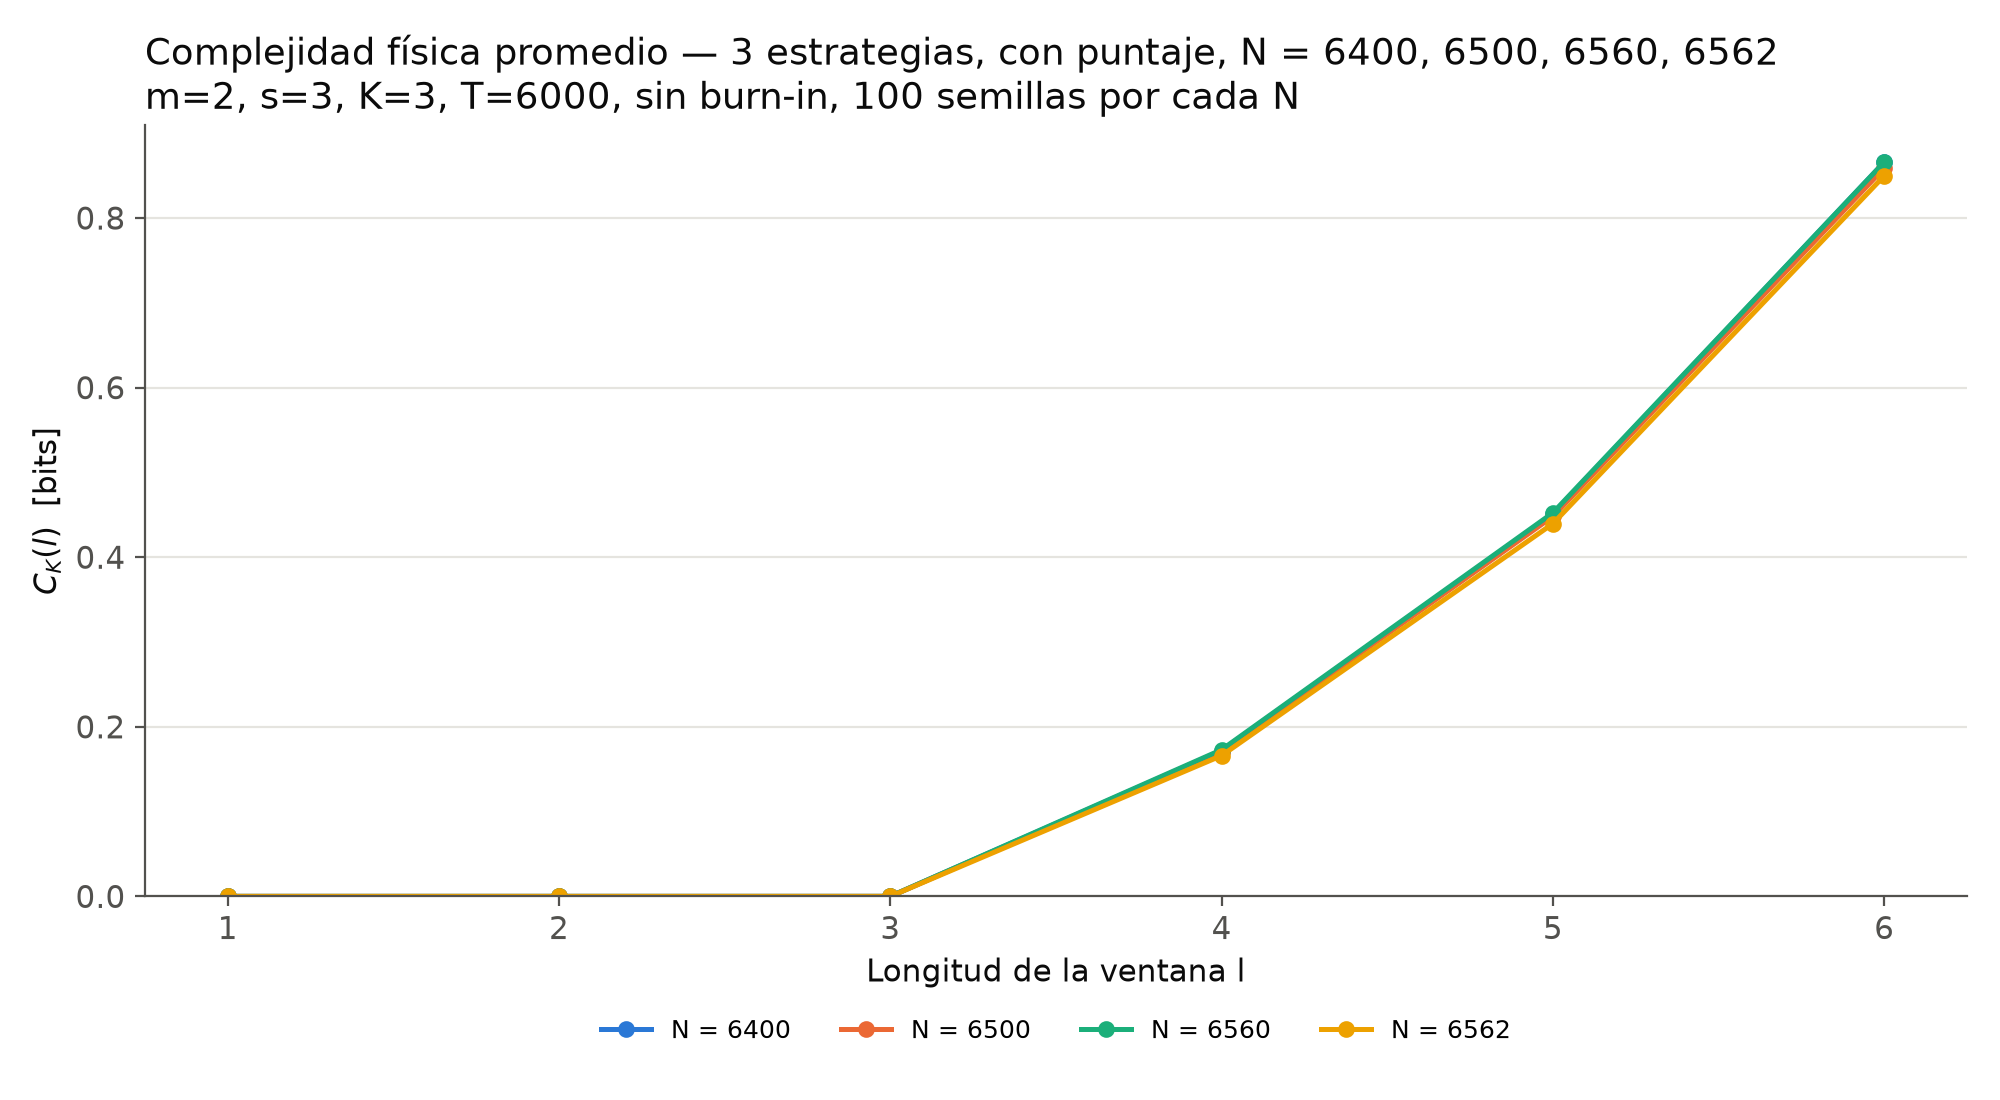
\includegraphics[width=0.49\textwidth]{figuras/Fase6_CK_con_puntaje_m2_s3_T6000_N6400-6500-6560-6562_promedio.png}
\caption{Fase 6, $N=6400, 6500, 6560, 6562$: $M(d)$ promedio (izquierda) y $C_K(l)$ promedio (derecha).}
\end{figure}
\begin{figure}[H]
\centering
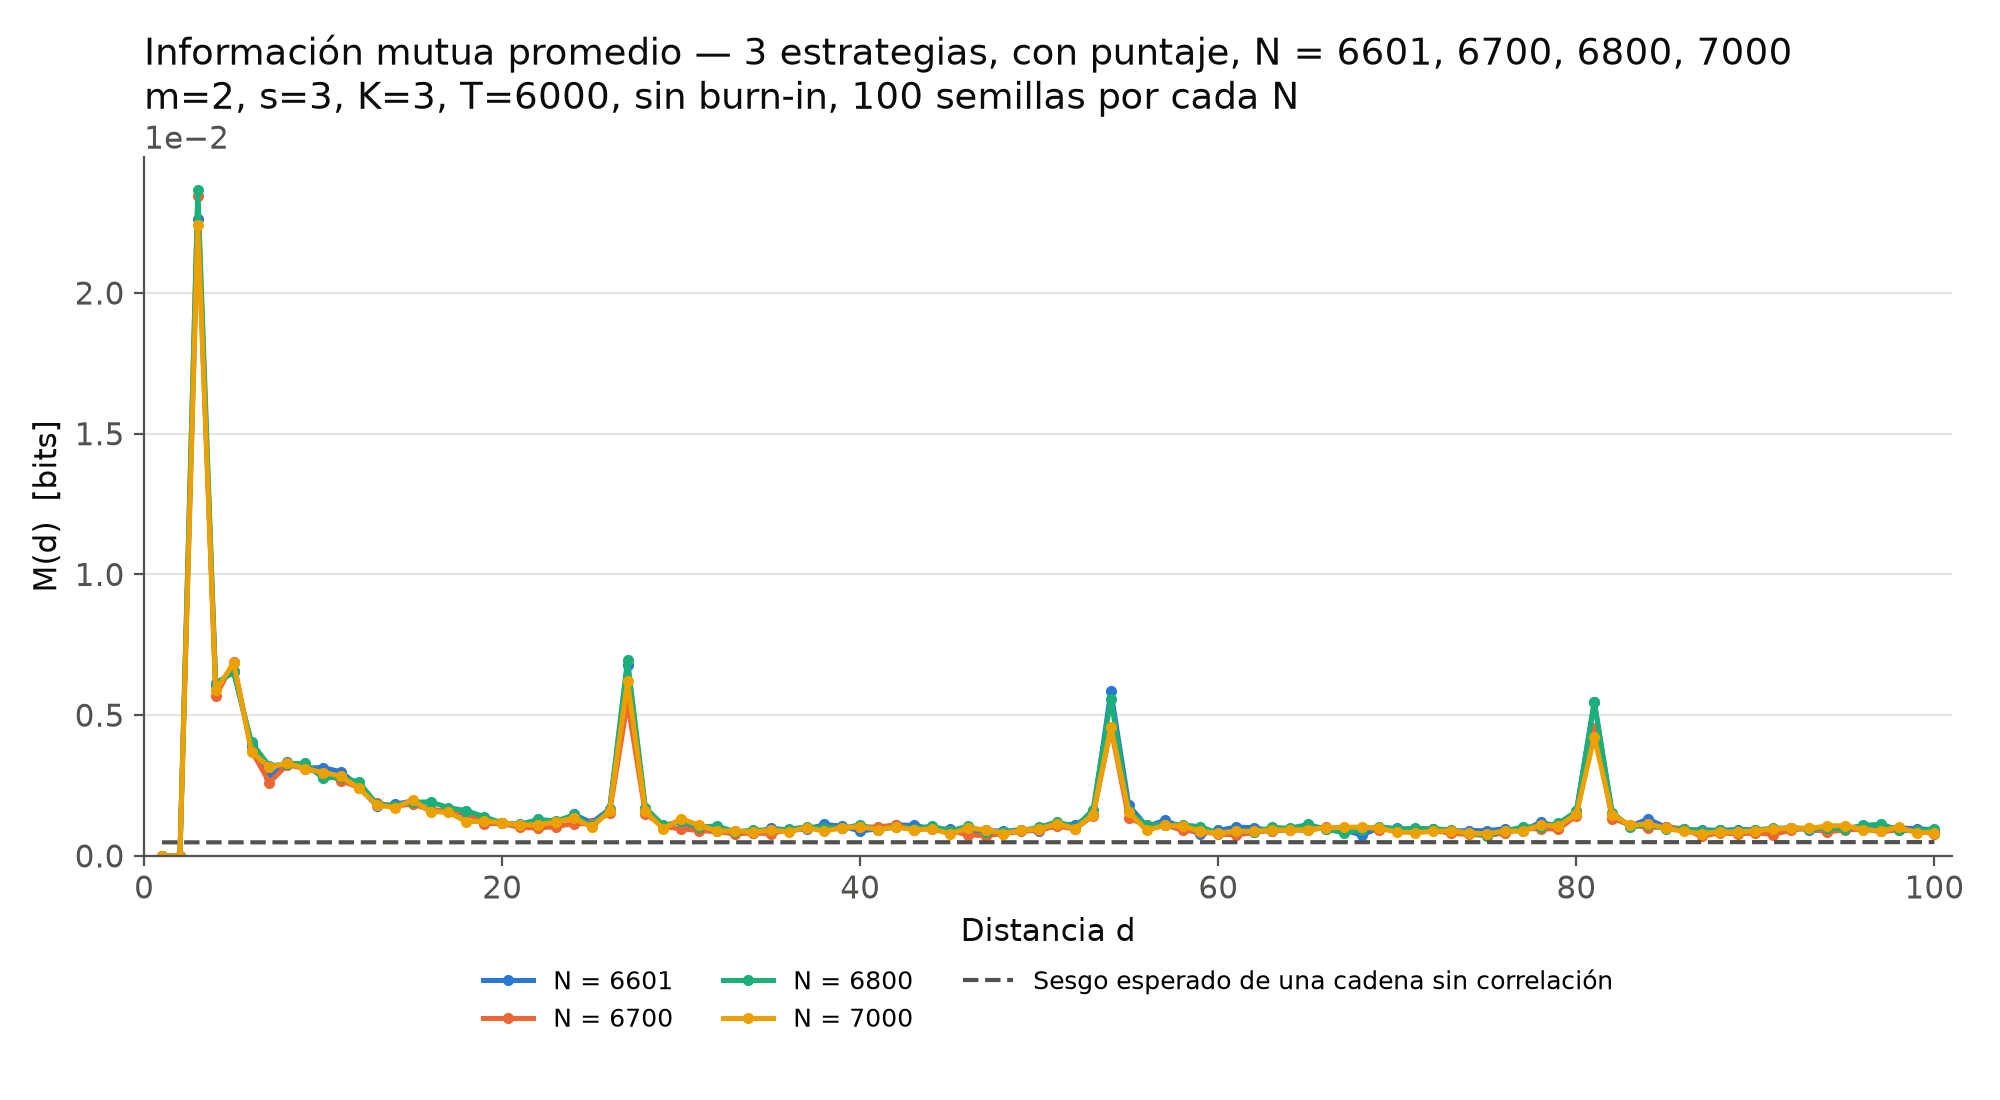
\includegraphics[width=0.49\textwidth]{figuras/Fase6_Md_con_puntaje_m2_s3_T6000_N6601-6700-6800-7000_promedio.png}\hfill
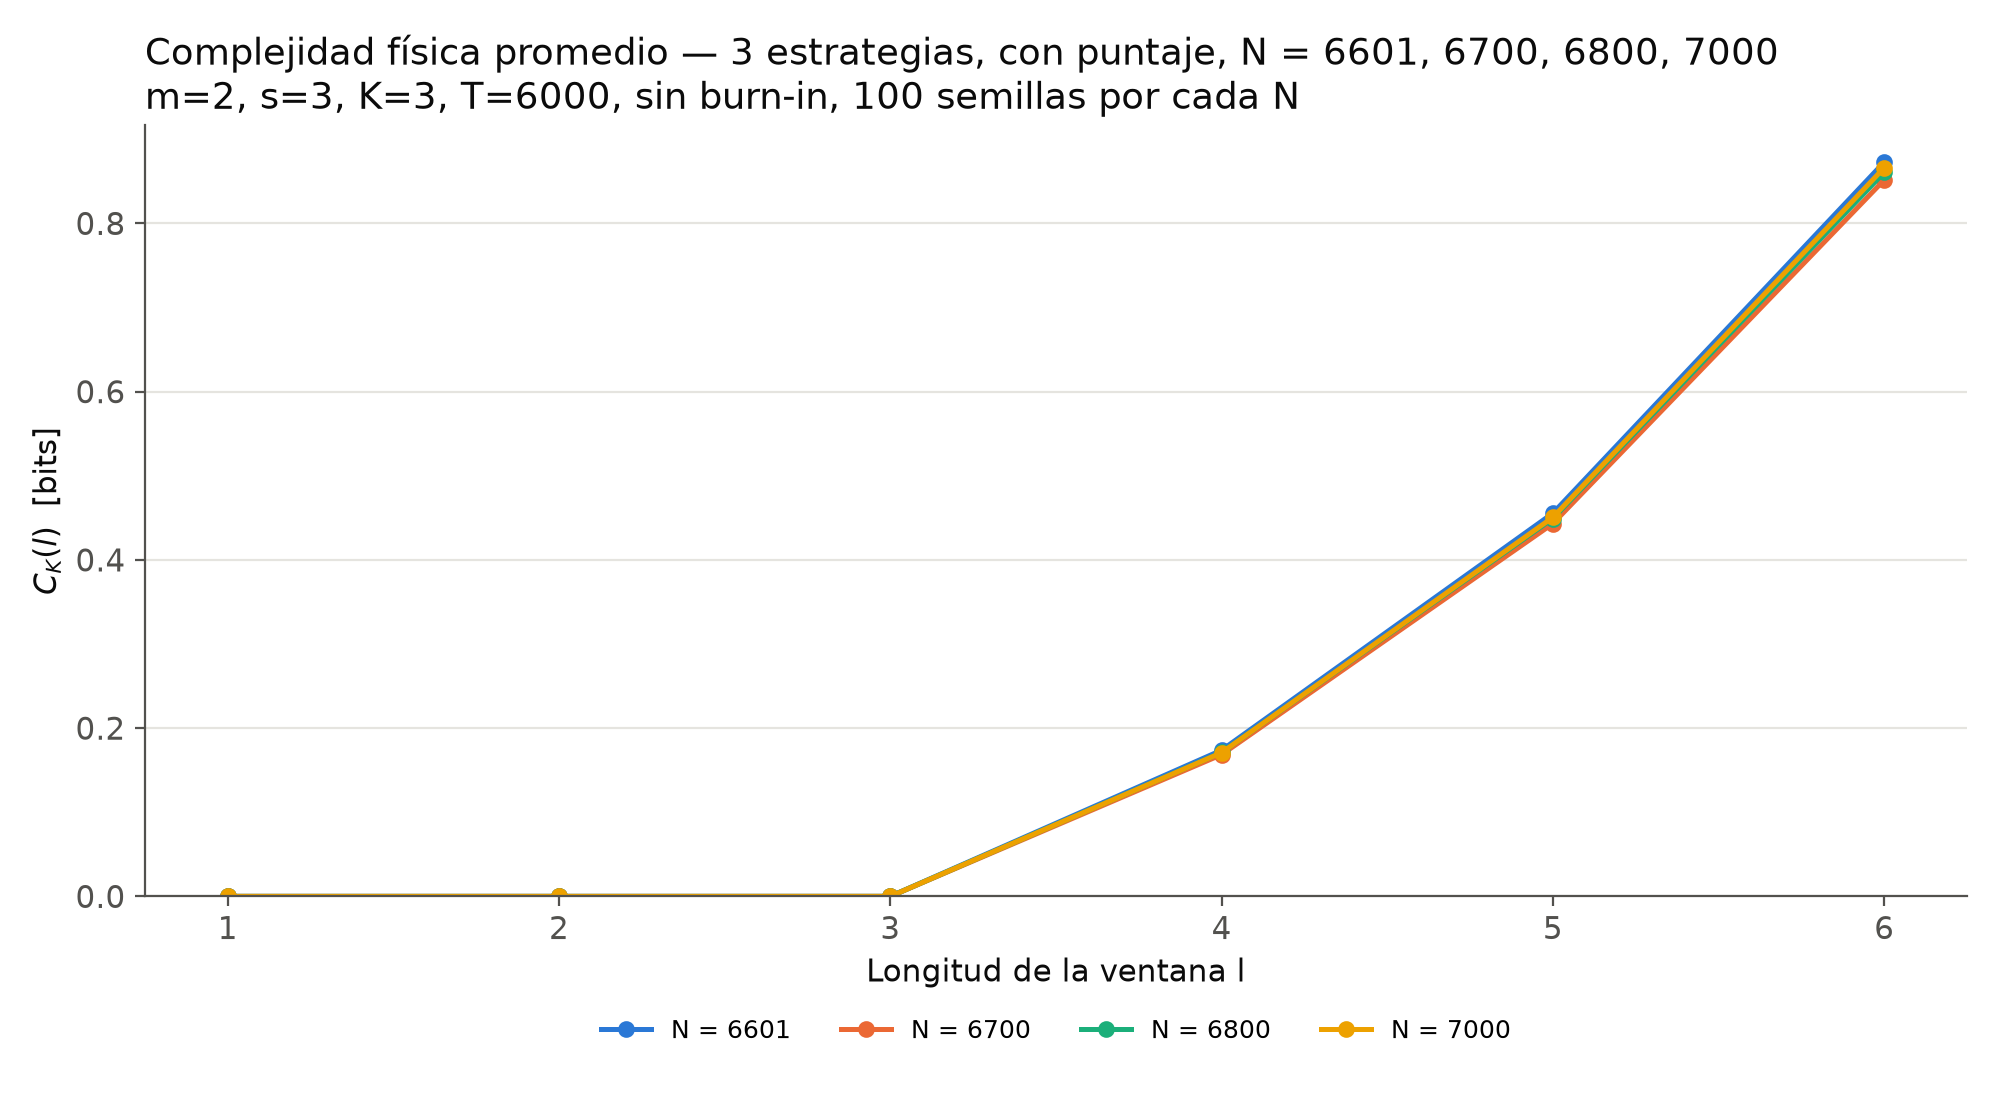
\includegraphics[width=0.49\textwidth]{figuras/Fase6_CK_con_puntaje_m2_s3_T6000_N6601-6700-6800-7000_promedio.png}
\caption{Fase 6, $N=6601, 6700, 6800, 7000$: $M(d)$ promedio (izquierda) y $C_K(l)$ promedio (derecha).}
\end{figure}


\end{document}
